%! Author = tstreule
%! Date = 18.01.22

\documentclass[%
,a4paper
,fontsize=8.6pt
,landscape
,pagesize
,headinclude
]{scrartcl}
\usepackage[margin=5mm,headsep=1mm,footskip=1mm]{geometry}

% Preamble and packages
%! Author = tstreule
%! Date = 17.01.22

% Language package
% \usepackage[utf8]{inputenc} % Not to use with Xe-LaTeX!
\usepackage{fontspec}
% \usepackage{kpfonts}
% \usepackage[T1]{fontenc}
\usepackage[english,ngerman]{babel}
\usepackage[svgnames]{xcolor}

% Flush left
\usepackage[document]{ragged2e}

% Set date format
\usepackage[useregional=numeric]{datetime2}

% Arithmetic / Coding package
\usepackage{ifthen}
\usepackage{calc}

% Spacing
\usepackage[nodisplayskipstretch]{setspace}
\setlength\intextsep{0pt}% no spacing above and below figures/tables
\setlength\columnsep{10pt}% Column spacing for multicols
% \setstretch{1.1}
% Move operators tighter together
\thinmuskip=2mu                     % default: 3mu
\medmuskip=3mu plus 1mu minus 3mu   % default: 4mu plus 2mu minus 4mu
\thickmuskip=4mu plus 3mu minus 3mu % default: 5mu plus 5mu
% \setlength{\thickmuskip}{5mu}     % not possible due to \usepackage{calc}
% Array and matrix spacing
\setlength\arraycolsep{1pt}
% Hack to remove vertical spacing in equations
\usepackage{etoolbox}
\newcommand{\setdisplayskips}{%
    \setlength{\abovedisplayskip}{1pt}%
    \setlength{\belowdisplayskip}{1pt}%
    \setlength{\abovedisplayshortskip}{1pt}%
    \setlength{\belowdisplayshortskip}{1pt}}
\appto{\normalsize}{\setdisplayskips}
\appto{\small}{\setdisplayskips}
\appto{\footnotesize}{\setdisplayskips}

% Control (primitive) list items
\usepackage{enumitem}
\setlist{leftmargin=*,nosep,labelsep=2pt,parsep=-0.2pt}  % reduce spaces
\setlist[itemize,2]{label=$\circ$}

% Formatting
\usepackage{multicol, multirow, tabularx}
\usepackage{makecell}
\usepackage{ulem} % for custom underline/strikethrough/...
\usepackage{float}

% Images
\usepackage{graphicx}

% Custom emphasizing
\colorlet{emph-text-color}{MediumOrchid}
\DeclareTextFontCommand{\emph}{\color{emph-text-color}\bfseries\sffamily}


% =============
% === FONTS ===

% Font sizes
\setkomafont{section}{\normalsize}
\setkomafont{subsection}{\normalsize}
\setkomafont{subsubsection}{\normalsize}
%\setkomafont{paragraph}{\normalsize}
%\setkomafont{subparagraph}{\normalsize}

% Set fonts
\setmainfont[LetterSpace=-1.5,WordSpace=0.8,Scale=1.0,
    BoldFont=* SemiBold,BoldItalicFont=* SemiBold Italic]{Noto Serif}
\setsansfont[LetterSpace=-1.8,WordSpace=0.8,Scale=1.0]{Open Sans}

\defaultfontfeatures{Mapping=tex-text}
\defaultfontfeatures{Ligatures=TeX}
\addfontfeature{LetterSpace=-20.0}


% ====================
% === TITLE FORMAT ===

\usepackage{titling}

% Reduce default vertical space before and after
\setlength{\droptitle}{-3.5em}
\renewcommand{\maketitlehookd}{\vspace{-1.3em}}

% Title
\pretitle{\centering\sffamily\large\bfseries}
\posttitle{\par}
% Author
\preauthor{\centering\sffamily\small}
\postauthor{\ifx\thedate\empty{\par}\else{}\fi}
% Date - remove spacing above and below
\predate{\centering\sffamily\small\ifx\thedate\empty{}\else{\;-\;}\fi\itshape}
\postdate{\ifx\thedate\empty{}\else{\par}\fi}


% =======================
% === SECTIONS FORMAT ===

% Make spacing tight
\RedeclareSectionCommands[%
    runin=false,
    beforeskip=1ex plus .5ex,
    afterskip=0ex plus .1ex,
]{section,subsection,subsubsection}

% Define colors
\colorlet{section-color}{RoyalBlue!90}
\colorlet{subsection-color}{RoyalBlue!40}
\colorlet{subsubsection-color}{RoyalBlue!20}
\colorlet{section-text-color}{white}
\colorlet{subsection-text-color}{black}
\colorlet{subsubsection-text-color}{black}

% Put in colored box with fixed height
\def\sectionboxheight{.7em}
\def\sectionboxvspace{-.1ex}
\makeatletter
\renewcommand\sectionlinesformat[4]{%
    \colorbox{#1-color}{%
        \begin{minipage}[b][\sectionboxheight][t]{\dimexpr\linewidth-2\fboxsep\relax}
            \vspace{\sectionboxvspace}%
            \raggedsection\color{#1-text-color}\@hangfrom{#3}{#4}%
            \vspace{\sectionboxvspace}%
        \end{minipage}%
    }}
\makeatother


% ===========================
% === HEADERS AND FOOTERS ===

\usepackage[footsepline]{scrlayer-scrpage}

\pagestyle{plain.scrheadings}

% Clear and set styles
\clearpairofpagestyles
%\clearscrheadfoot
\setkomafont{pageheadfoot}{\color{gray}\sffamily}

% Reset pagination format
\setkomafont{pagination}{}

% Set content
%\ihead*{}
%\chead*{}
%\ohead*{tstreule $\vert$ Page \pagemark}
%\ifoot*{}
%\cfoot*{}
%\ofoot*{}


% =====================
% === COLOR STYLING ===
% \everymath\expandafter{\the\everymath\color{MediumBlue}}
% --> use "\the\everymath" for default math color
% --> use "\normalcolor" for other way around

\usepackage{../shortcuts}

% Uncomment for debugging headers
% \usepackage{showframe}

\graphicspath{{./graphics/}} % Set graphic path

% >>> [BEGIN] (Re-)formatting >>>
\setmainfont[LetterSpace=-2,WordSpace=0.8,Scale=1.0,
	BoldFont=* SemiBold,BoldItalicFont=* SemiBold Italic]{Noto Serif}
\let\degree\relax\usepackage{mathabx}
\usepackage{siunitx,amscd,esint,svg,wasysym}
\usepackage[version=4]{mhchem}
\newlength{\boxmargin}
\setlength{\boxmargin}{2pt}
%\parskip\boxmargin
% same parskip inside minipage
\makeatletter
\let\org@parboxrestore\@parboxrestore
\def\@parboxrestore{%
	\edef\restore@parsettings{%
		\parindent=\the\parindent\relax
		\parskip=\the\parskip\relax
	}%
	\org@parboxrestore
	\restore@parsettings
}
\makeatother
\parindent0pt
\unitlength10mm
\newcommand{\formulaEnvironment}[3][]{\par
	\parbox{0.3\columnwidth}{\raggedright#2}\hspace{\boxmargin}#3%
	\ifthenelse{\not\equal{#1}{}}{%
		\hspace{\boxmargin}$\left[#1\right]$}{}}
\newcommand{\formula}[3][]{%						'\formula'		% formula
	\formulaEnvironment[#1]{#2}{$#3$}}
\newcommand{\formbox}[3][]{%						'\formbox'		% eqbox in formula style
	\formulaEnvironment[#1]{#2}{\highlight{$\!\!#3\!\!$}}}
\newcommand{\formtex}[2]{%						'\formtex'		% text in formula style
	\formulaEnvironment{#1}{#2}}
% <<< [END] (Re-)formatting <<<

% Set title
\title{Bioelectronics}
\author{Timo Streule, tstreule@ethz.ch}
\date{\today}

% ======================
% === BEGIN DOCUMENT ===

\begin{document}

	%! Author = tstreule
%! Date = 17.01.22

\providecommand\thetitle{LECTURE\_NAME}

\begingroup
%\vspace*{\fill}
%\begin{center}
\begin{minipage}{.35\textwidth}

    \setmainfont{Noto Serif}
    \KOMAoptions{fontsize=12pt}\color{black}
    \justifying

    {\Large\bfseries Disclaimer}

    This document is an exam summary and follows the given material of the lecture {\itshape \thetitle}.
    Its contribution is a short summary that contains the most important concepts, formulas and algorithms.
    Due to curriculum content updates, some content may not be relevant to future versions of the course.

    I do not guarantee the accuracy or completeness, nor is this document endorsed by the instructors.
    Any errors that are pointed out to me are welcome.
    The complete {\LaTeX} source code can be found at {\ttfamily https://github.com/tstreule/eth-cheat-sheets}.

\end{minipage}
%\end{center}
%\vspace*{\fill}
\endgroup

\pagebreak


	\begin{multicols*}{3}

		% Suppress enumeration of sections
		%\setcounter{secnumdepth}{0}

		\maketitle

		%! Author = tstreule

\section*{General}

\subsection*{Formeln}
%
\textbf{Circle}: $U\ped{circle} = 2\pi r$, $A\ped{circle} = \pi r^2$

%	\textbf{Laplace}:\\
%	\begin{tabular}{ c@{$\;\laplace\;$}c c c@{$\;\laplace\;$}c }
%		$f(at)$			& $\frac{1}{\abs{a}}F(s/a)$	&& $f(t-a)$		& $\eu^{-as}F(s)$\\
%		$f(t)\eu^{at}$	& $F(s-a)$					&& $f'(t)$		& $sF(s) - f(0^+)$\\
%		$t^n$			& $n!/s^{n+1}$				&& $t^n f(t)$	& $(-1)^n F^{(n)}(s)$\\
%		$\sin(at)$		& $\frac{a}{s^2 + a^2}$		&& $\cos(at)$	& $\frac{s}{s^2 + a^2}$\\
%		$\eu^{at}$		& $\frac{1}{s - a}$			&& $t^n \eu^{at}$& $\frac{n!}{(s-a)^{n+1}}$
%	\end{tabular}

\textbf{Constants}:\\
\begin{tabular}{r@{$\;=\;$}l}
    $h$			& $\unit[6.626 {\scriptstyle\mathrm{E}-34}]{Js} = \unit[4.135 {\scriptstyle\mathrm{E}-15}]{eV\,s}$,
    \quad $\hbar = \frac{h}{2\pi}$,
    \quad $hc = \unit[1.986 {\scriptstyle\mathrm{E}-25}]{Jm}$\\
    $\epsilon_0$& $\unitfrac[8.85 {\scriptstyle\mathrm{E}-5}]{As}{Vm}$\\
    $\mu_0$		& $\unitfrac[4\pi {\scriptstyle\mathrm{E}-7}]{N}{A^2}$\\
    $k\ped{B}$	& $\unitfrac[1.38 {\scriptstyle\mathrm{E}-23}]{J}{K} = \unitfrac[8.617 {\scriptstyle\mathrm{E}-5}]{eV}{K}$\\
    $q$			& $\unit[1.602 {\scriptstyle\mathrm{E}-19}]{C}$, \quad $m_e = \unit[9.109 {\scriptstyle\mathrm{E}-31}]{kg}$, \quad $m_p = \unit[1.672 {\scriptstyle\mathrm{E}-27}]{kg}$\\
    $F$			& $\unitfrac[96485]{C}{mol}$ (Faraday)\\ % charge of 1 mole of electrons
    $R$         & $N\ped{A} k\ped{B} = \unitfrac[8.314]{J}{mol\;K}$ (Ideal gas constant)\\
    $N\ped{A}$	& $\unitfrac[6.022 {\scriptstyle\mathrm{E}23}]{particles}{mol}$
    \qquad $\SI{0}{\degreeCelsius} = \unit[273.15]{K}$
\end{tabular}
%%%%%%%%%%%%%%%%%%%%%%%%%%%%%%%%%%%%%%%%%%%%%%%%%%%%%%
\subsection*{Einheiten}
%
\formula{Druck}{\unit[1]{Pa} = \unitfrac[1]{N}{m^2} = \unitfrac[1]{J}{m^3} = \unitfrac[10]{g}{cm\cdot s^2}}\\
\formula{Induktivität}{\unit[1]{H} = \unitfrac[1]{Vs}{A} = \unit[1]{\Omega\,s}}\\
\formula{Power}{\unit[1]{W} = \unitfrac[1]{J}{s} = \unit[1]{VA}}\\
\formula{electron volt}{\unit[1]{eV} = \unit[1.602 {\scriptstyle\mathrm{E}-19}]{J} = \unitfrac[23.06]{kcal}{mol}}\\
\formula{Charge}{\SI{1}{\coulomb} = \SI{1}{\ampere\second}}\\
\formula{Energy}{\SI{1}{\joule} = \unitfrac[1]{kg\;m^2}{s^2} = \unit[1]{Nm} = \unit[1]{VAs} = \unit[1]{CV} = \unit[1]{Ws}}\\
%%%%%%%%%%%%%%%%%%%%%%%%%%%%%%%%%%%%%%%%%%%%%%%%%%%%%%
\subsection*{Good to know}
%
\formula{Power in \unit{dB}}{10\,\log_{10}\frac{I}{I_0}}\\
\formula[\unit{\frac{\!W}{m^2}}]{Intensity}{ I = \frac{\textrm{avg. Power }(P)}{\textrm{area }(A)} }\\
\formula[\unit{W} = \unit{\frac{kg\,m^2}{s^3}}]{avg. Power}{P = \frac{\textrm{avg. Work in cycle }(\overline{W})}{\textrm{cycle }(T)}}\\
\formula[\unit{J}=\unit{Ws}]{(avg.) Work}{\overline{W} = \int_{\textrm{cycle}} \frac{1}{\textrm{cycle} (T)} \cdot \vec{F}\cdot\vec{x} \diff t }\\

mass $m$ vibrates with an amplitude $a$ along $x$-axis:\\
$\vec{x}(t) = a\sin(\omega t)\cdot \vec{e}_x, \quad \omega = 2\pi f = 2\pi/T, \quad \vec{F}(t) = m\,\ddot{\vec{x}}(t)$
%%%%%%%%%%%%%%%%%%%%%%%%%%%%%%%%%%%%%%%%%%%%%%%%%%%%%%
\subsection*{NuS}
%
\formula{Induktivität}{u(t) = L \deriv{i_L}{t} \enskip\laplace\enskip U(s) = sL\,I_L(s)}\\
\formula{Konduktivität}{i(t) = C \deriv{u_C}{t} \enskip\laplace\enskip U(s) = \frac{1}{sC}\,U_C(s)}\\

\formula{Transformator}{u_1 = L_1 \deriv{i_1}{t} - M \deriv{i_2}{t} \textnormal{,\enskip $M$: mutual inductance}}\\
\formula{LCR-Schwingkreis}{\omega_0 = 2\pi f_0 = 1/\sqrt{LC}}\\
%%%%%%%%%%%%%%%%%%%%%%%%%%%%%%%%%%%%%%%%%%%%%%%%%%%%%%
\subsection*{Laplace}
%	%Laplace Transformation: \;
%	$\phantom{\laplace} \dis{0.4} u(t)=\mathcal{L}^{-1}\{U(s)\} = \frac{1}{2\pi\iu} \int_{\bar{s}}^s U(s)\eu^{st} \diff s$\\
%	$\laplace \dis{0.4} U(s)=\mathcal{L}\{u(t)\} = \int_0^\infty u(t)\eu^{-st} \diff t$
%
\begin{tabular}{ rcl }
    \toprule
%		$u(t)$							& \laplace	& $U(s)$								\\%\addlinespace
%		\midrule
    $\lambda\;u(t) + \mu\;v(t)$		& \laplace	& $\lambda\;U(s) + \mu\;V(s)$			\\
    ${u(at),\; \scriptstyle a>0}$	& \laplace	& $\frac{1}{a}$ $U(\frac{s}{a})$		\\
    { \color{red} $u(t-t_0)$ }		& \laplace	& $\eu^{-st_0}$ $U(s)$					\\
    $\eu^{-at}$ $u(t)$				& \laplace	& { \color{red} $U(s+a)$ }				\\
    ${ (-t)^{n} u(t) }$				& \laplace	& $U^{(n)}(s)$							\\
    $u^{(n)}(t)$					& \laplace	& $ {s^nU(s) - \ldots - u^{(n-1)}(0)} $	\\
    \midrule
%		$t^n$							& \laplace	& $\frac{n!}{s^{n+1}}$					\\\addlinespace
%		$\eu^{-at}$						& \laplace	& $\frac{1}{s+a}$						\\\addlinespace
%		$t\eu^{-at}$					& \laplace	& $\frac{1}{(s+a)^2}$					\\\addlinespace
%		$t^n\eu^{-at}$					& \laplace	& $\frac{n!}{(s+a)^{n+1}}$				\\\addlinespace
%		$\sin (at)$						& \laplace	& $\frac{a}{s^2+a^2}$					\\\addlinespace
%		$\cos(at)$						& \laplace	& $\frac{s}{s^2+a^2}$					\\\addlinespace
    \multicolumn{3}{c}{
        \begin{minipage}{.45\columnwidth} \centering
        \begin{tabular}{ ccc }
%					$u(t)$							& \laplace	& $U(s)$								\\%\addlinespace
%					\midrule
            $t^n$							& \laplace	& $\frac{n!}{s^{n+1}}$					\\
            $\eu^{-at}$						& \laplace	& $\frac{1}{s+a}$						\\
            $t\eu^{-at}$					& \laplace	& $\frac{1}{(s+a)^2}$					\\
        \end{tabular}
        \end{minipage}%
        \begin{minipage}{.45\columnwidth} \centering
        \begin{tabular}{ ccc }
%					$u(t)$							& \laplace	& $U(s)$								\\%\addlinespace
%					\midrule
            $t^n\eu^{-at}$					& \laplace	& $\frac{n!}{(s+a)^{n+1}}$				\\
            $\sin (at)$						& \laplace	& $\frac{a}{s^2+a^2}$					\\
            $\cos(at)$						& \laplace	& $\frac{s}{s^2+a^2}$					\\
        \end{tabular}
        \end{minipage}
    }\\
    \bottomrule
\end{tabular}

		%! Author = tstreule

\section{Biosensors}
%%%%%%%%%%%%%%%%%%%%%%%%%%%%%%%%%%%%%%%%%%%%%%%%%%%%%%
%%%%%%%%%%%%%%%%%%%%%%%%%%%%%%%%%%%%%%%%%%%%%%%%%%%%%%
%	\subsection{Biosensors Principle}
%	%
%	\begin{center}
%		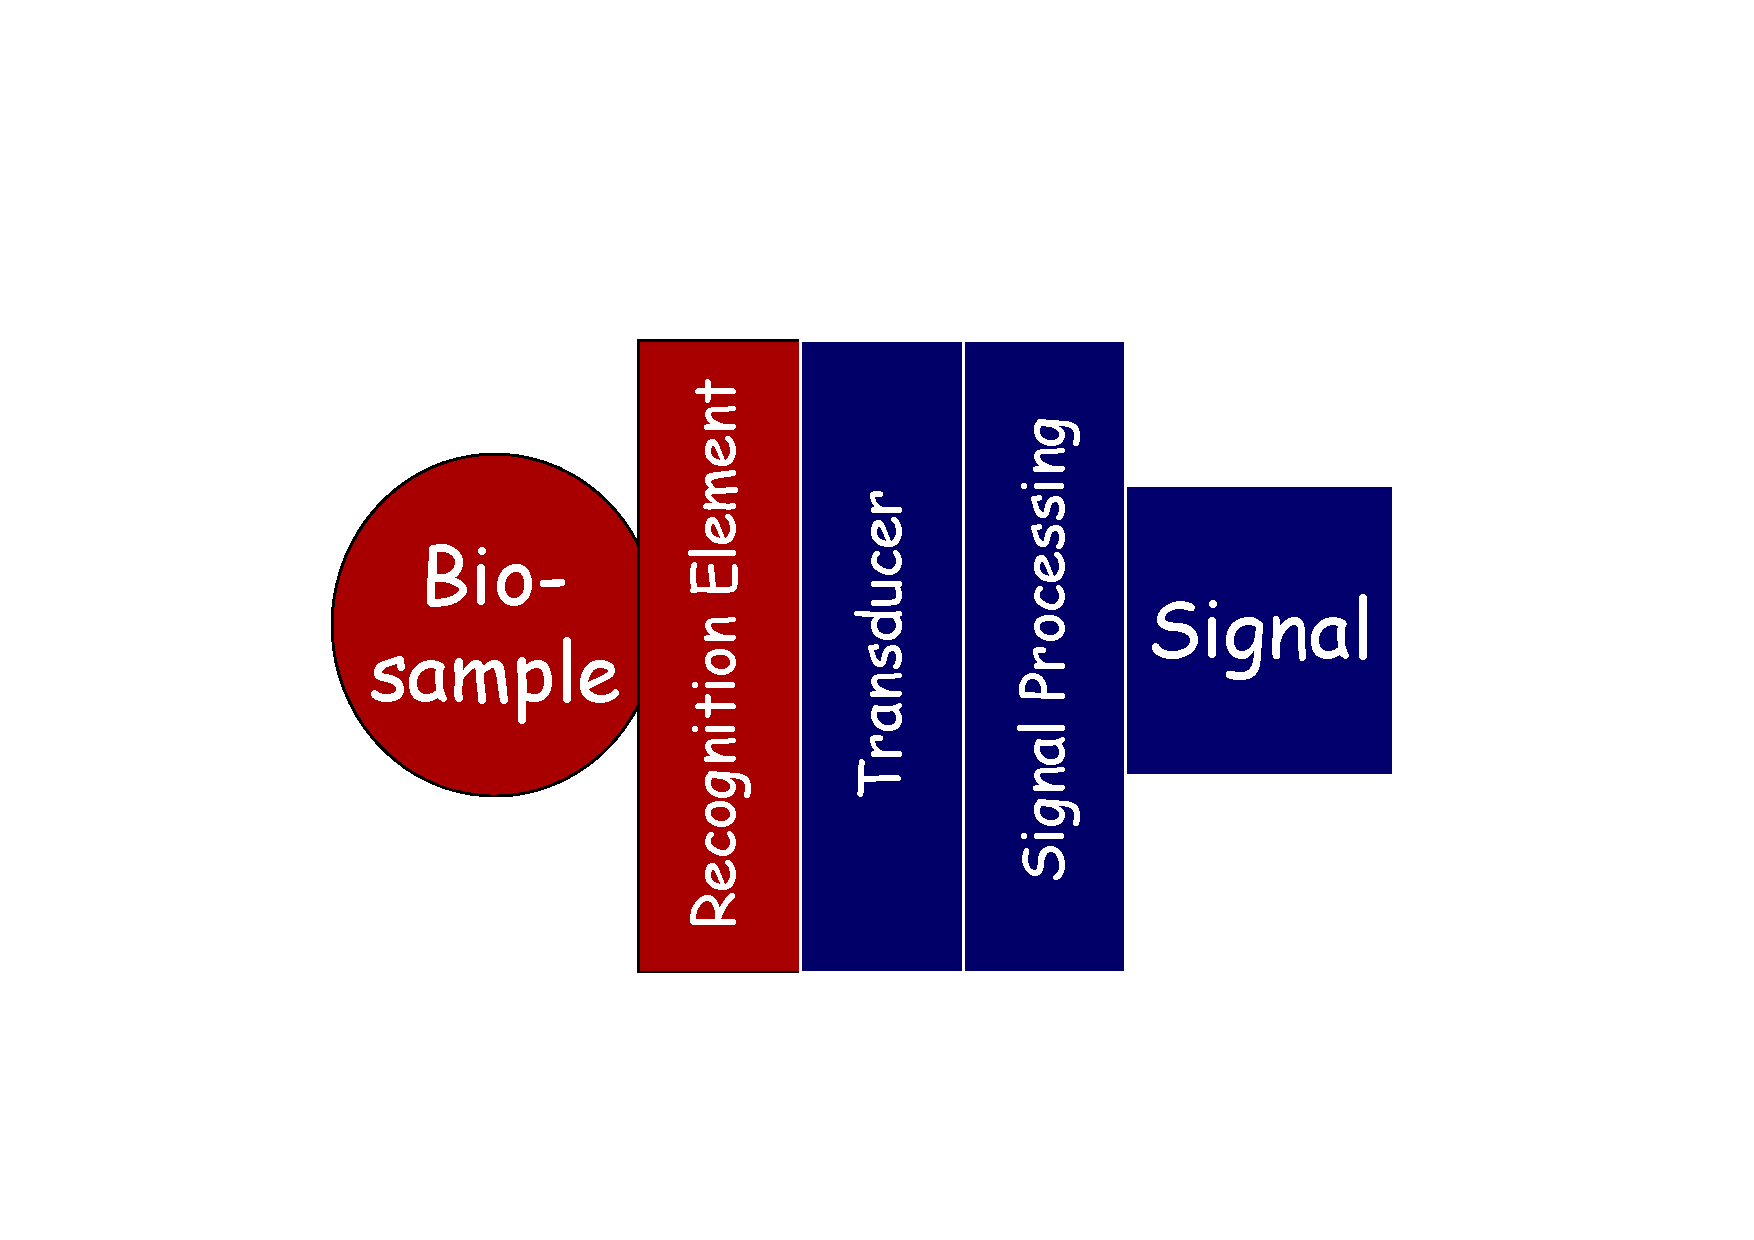
\includegraphics[width=.3\columnwidth]{Biosensors_Principle}
%	\end{center}
%%%%%%%%%%%%%%%%%%%%%%%%%%%%%%%%%%%%%%%%%%%%%%%%%%%%%%
\subsection{Label assay vs. label-free}
%
\shortstack{Label assay\\(sandwich):}
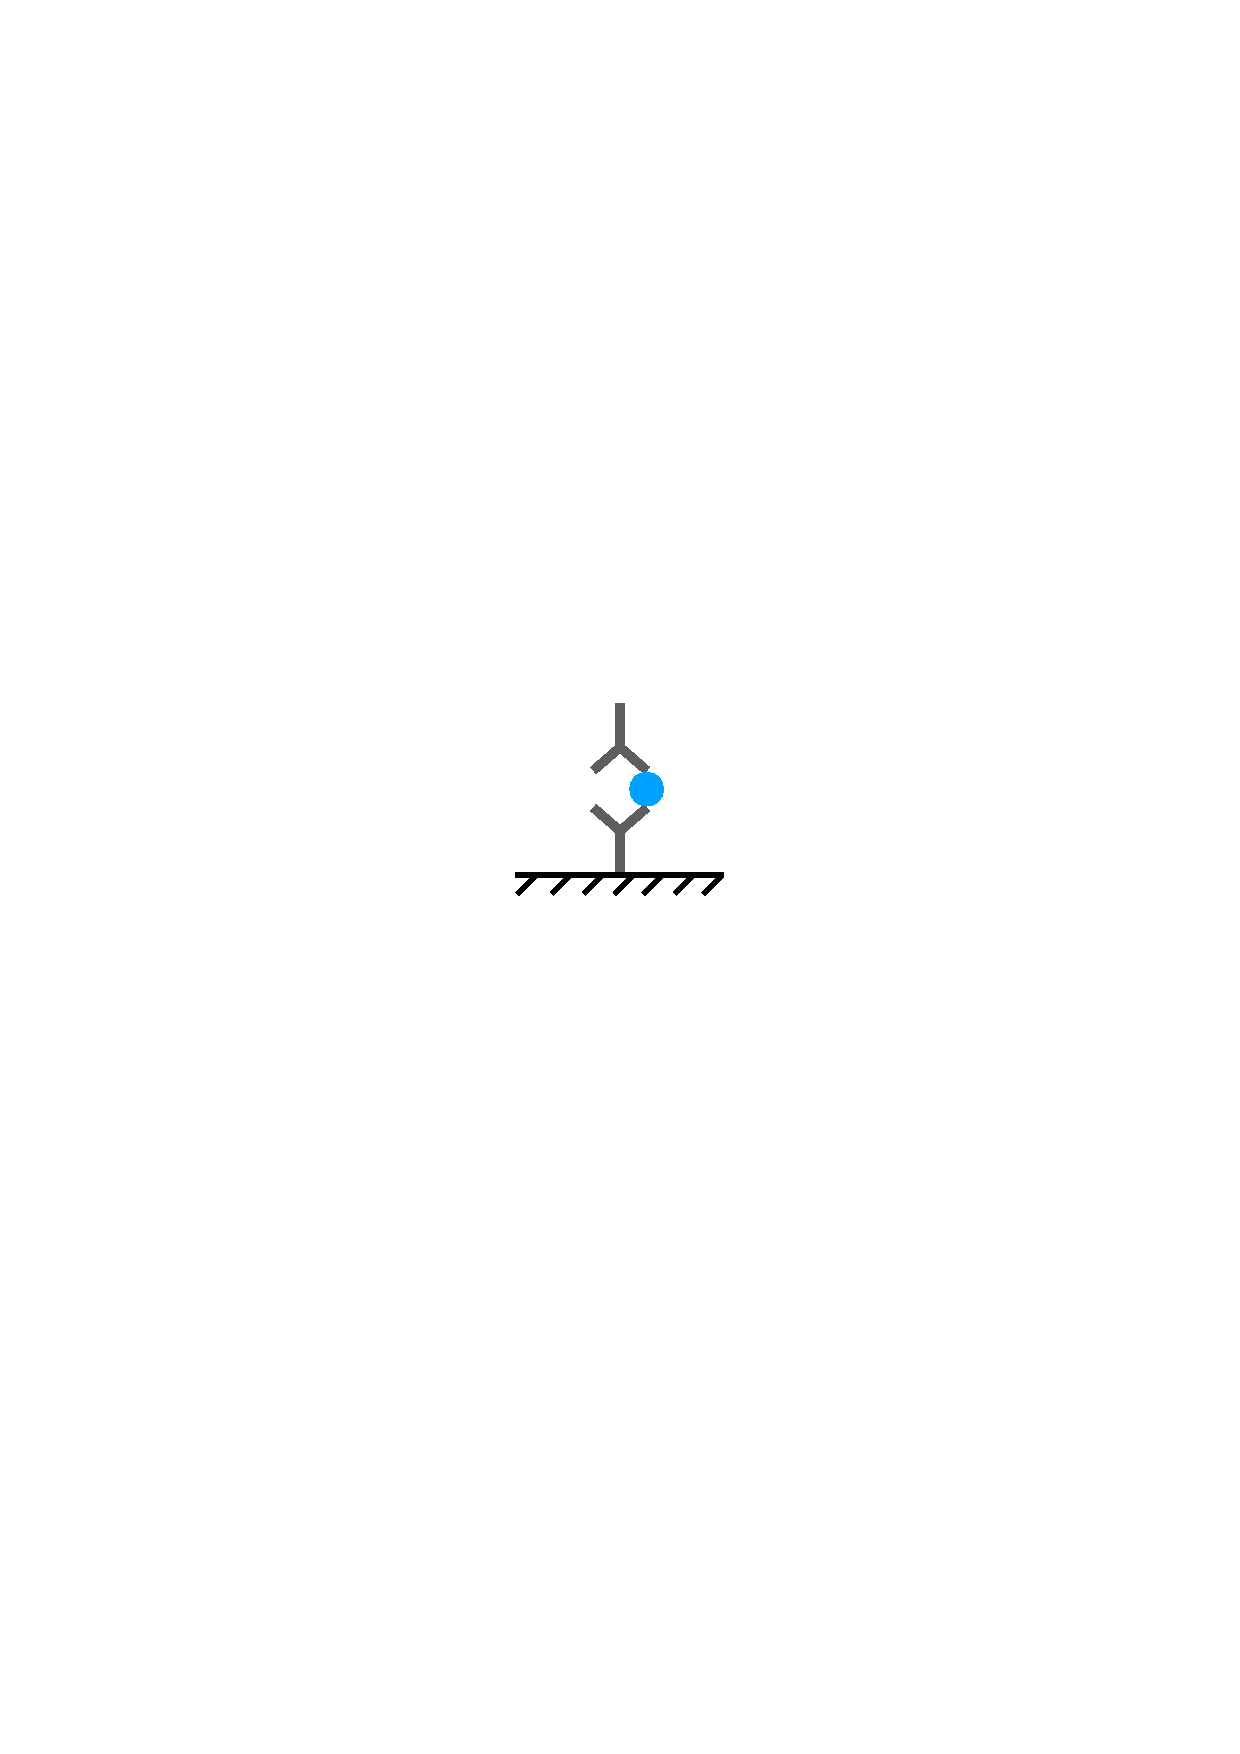
\includegraphics[width=.08\columnwidth]{Biosensors_Label_Assay}
\qquad
\shortstack{Label-free assay\\(OWLS):}
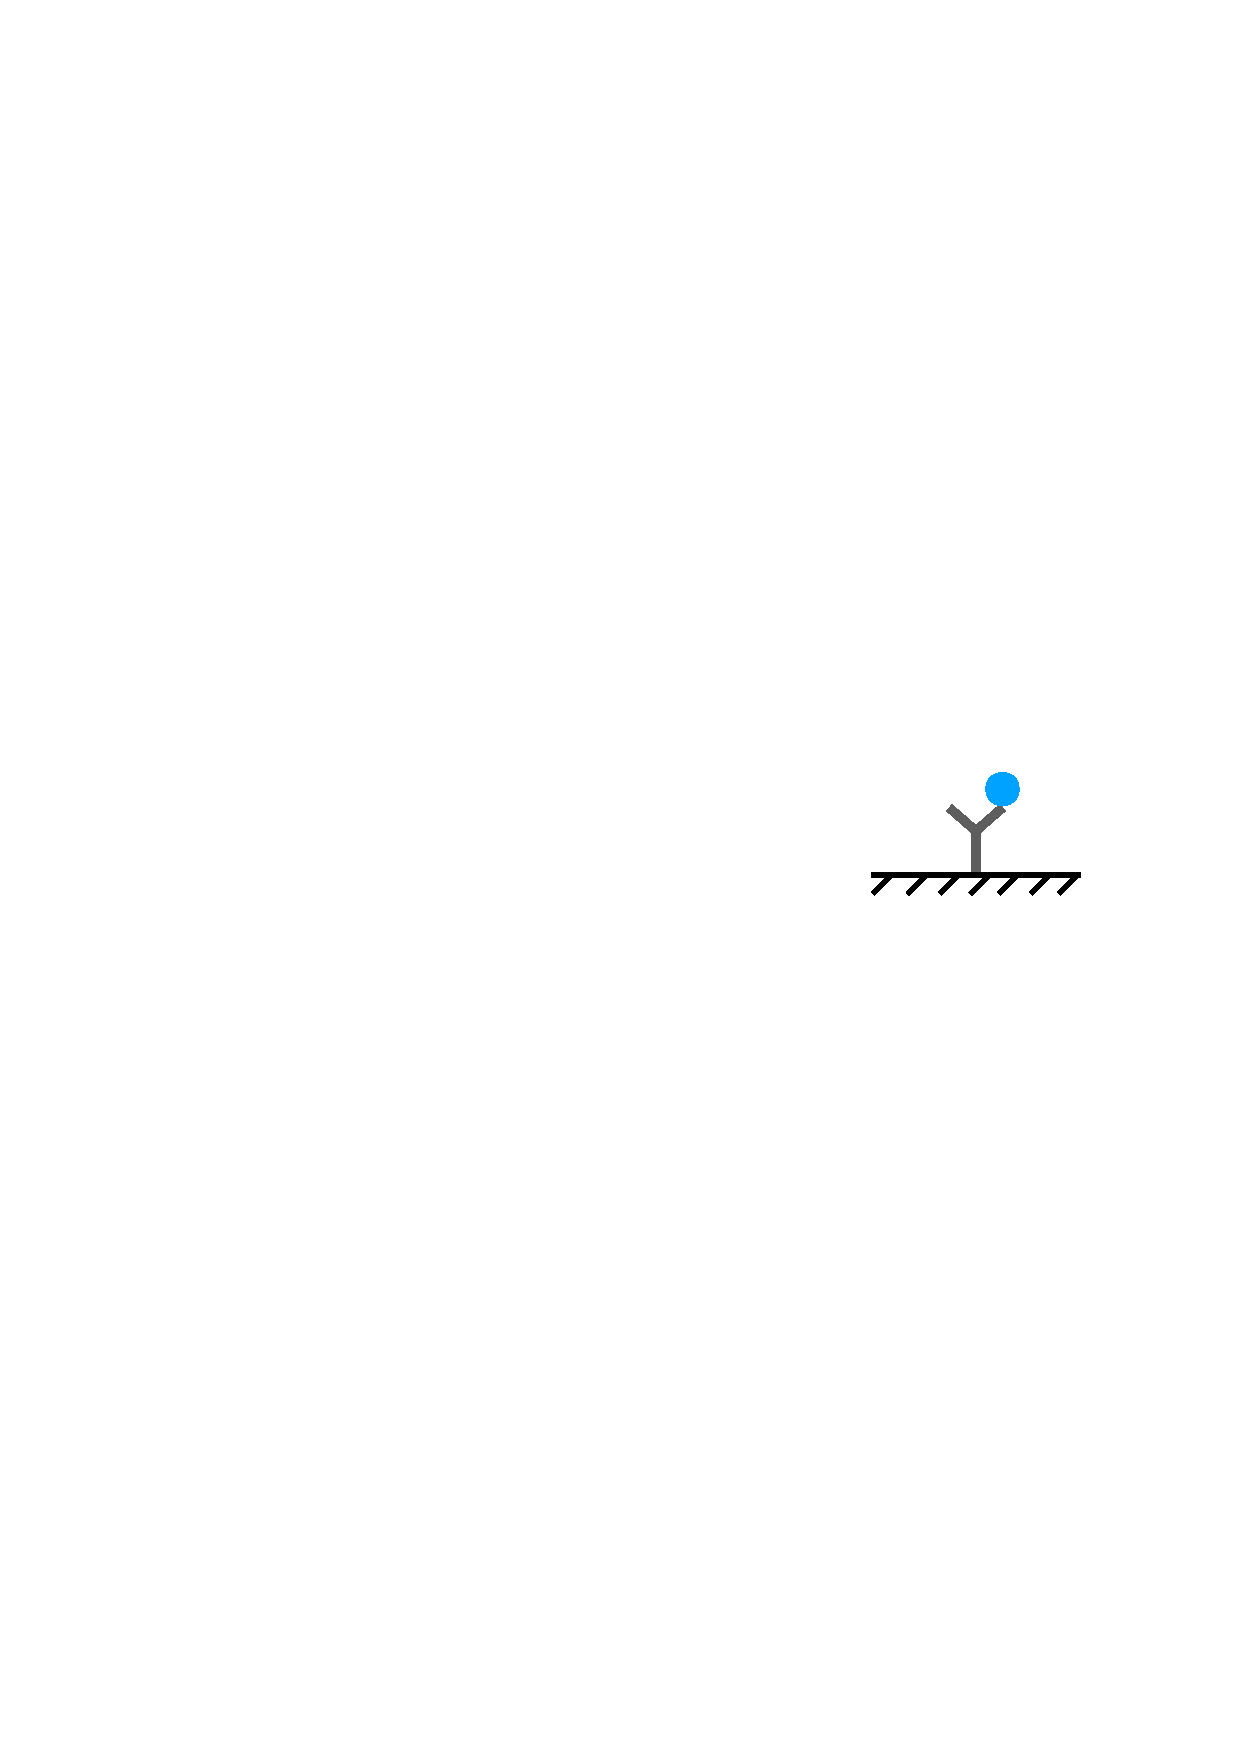
\includegraphics[width=.08\columnwidth]{Biosensors_Label_Free}
\par
\shortstack{non-specific\\binding:}
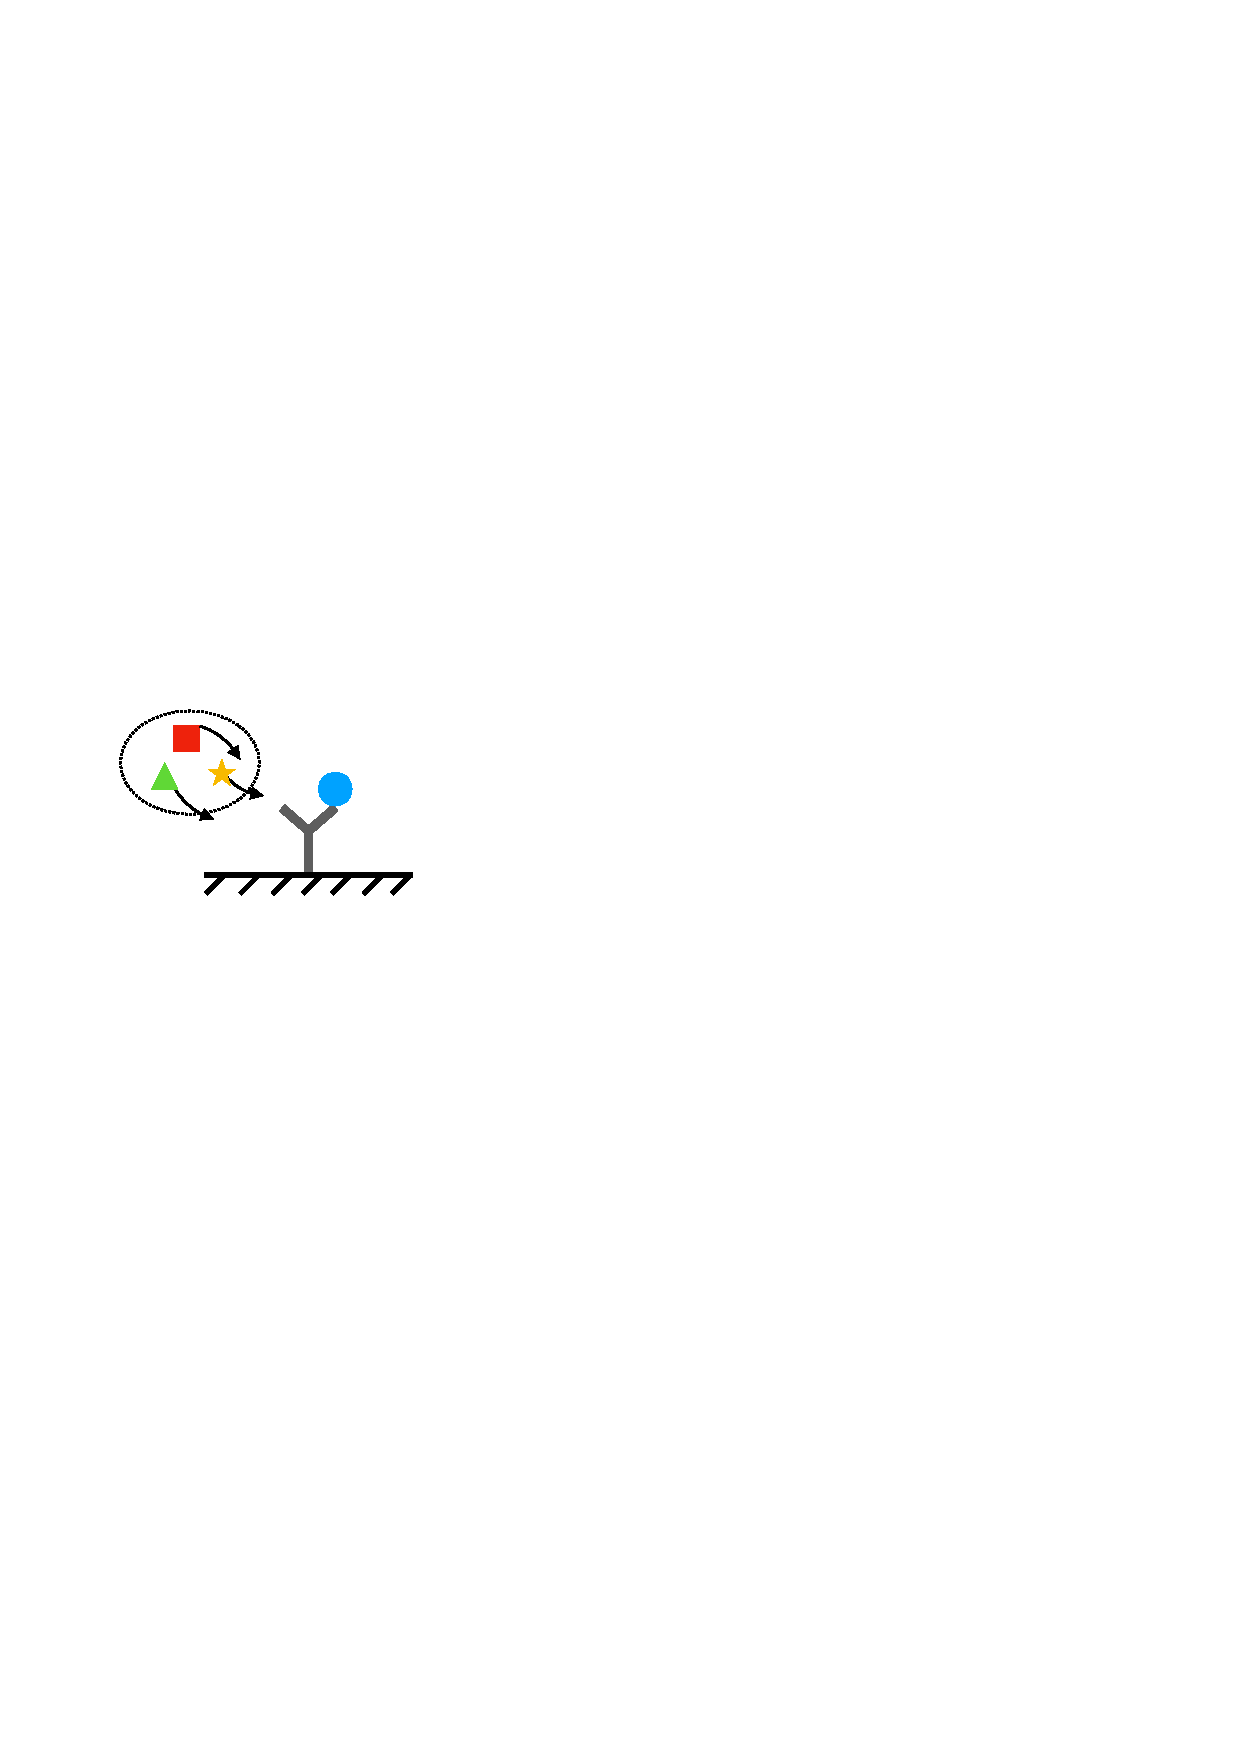
\includegraphics[width=.12\columnwidth]{Biosensors_Non_Specific}
\shortstack[r]{other interactions that could happen,\\ except the angle binding.}
%%%%%%%%%%%%%%%%%%%%%%%%%%%%%%%%%%%%%%%%%%%%%%%%%%%%%%
\subsection{Rules of Chemistry and Physics}
%
\formtex{\textit{Bracket notation}}{indicates concentration}
\ce{A +B <=>[$k_1$][$k_{-1}$] AR}
\formbox{equilibrium constant}{K = \frac{k_{-\!1}}{k_1} = \frac{[A][R]}{[AR]}}
\formula{affinity constant}{K_a = 1/K}
\formula{cont. flowing cell}{[AR] \sim q * \text{signal},}
$q=const$
\formula{~}{[R] \sim R_0 = \text{initial receptor density}}
%
%	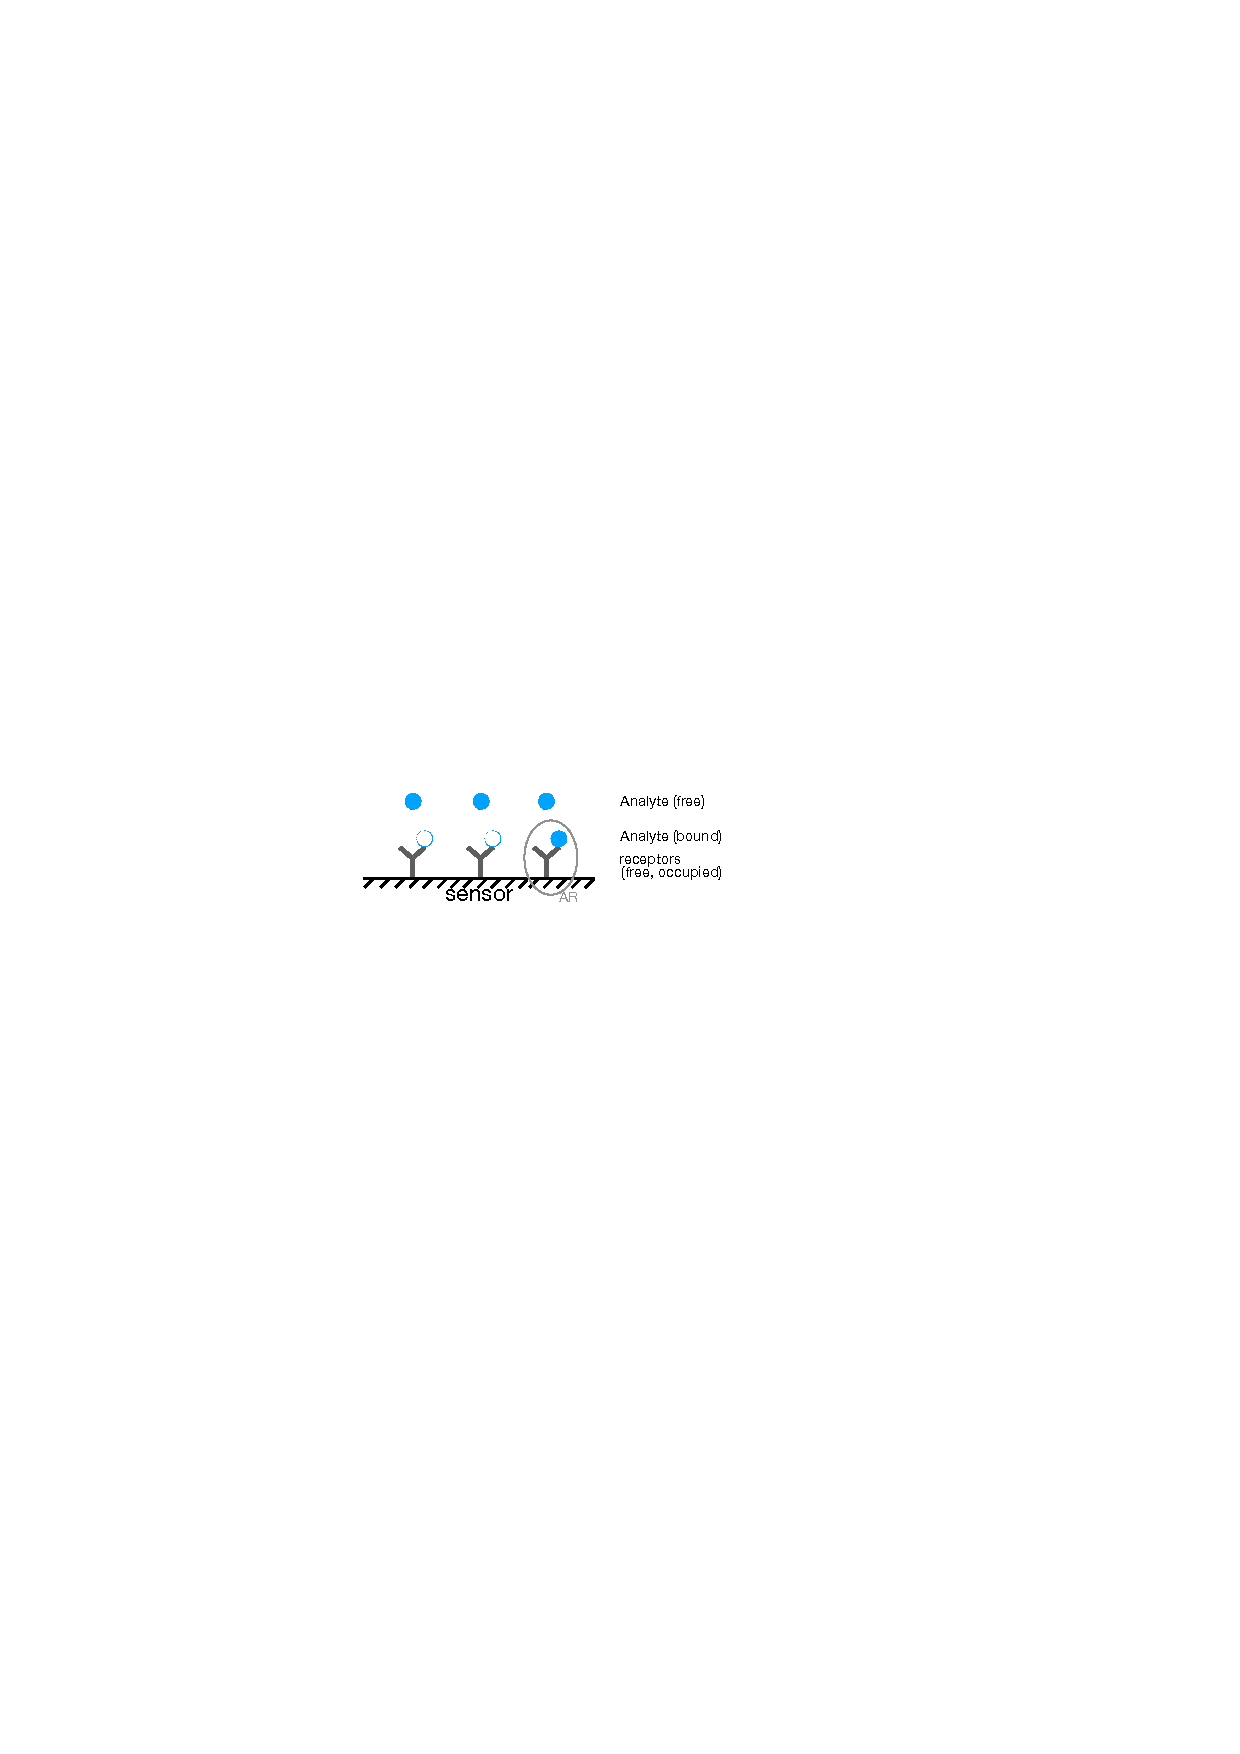
\includegraphics[width=.6\columnwidth]{Biosensors_Rules_of_Chemistry}
%%%%%%%%%%%%%%%%%%%%%%%%%%%%%%%%%%%%%%%%%%%%%%%%%%%%%%
\subsection{Sensitivity and Specificity}
%
%	All biosensing techniques are limited by the non-specific interaction = “It is not possible to catch \underline{only} Nemo with a fishing net”
%
\formula{Sensitivity}{\text{true positive rate (\% of correctly identified $+$)}}
\formula{Specificity}{\text{true negative rate (\% of correctly identified $-$)}}

Compensate Sensitivity through LOD.
%%%%%%%%%%%%%%%%%%%%%%%%%%%%%%%%%%%%%%%%%%%%%%%%%%%%%%
\subsubsection{Limit of Detection (LOD) \hfill \textnormal{(Sensitivity)}}
%
Limitation by non-specific binding (NSB) $\to$ noise at zero analyte

\begin{minipage}{.65\columnwidth}
    \formula{LOD}{LOD = 3\cdot\textrm{noise} / \deriv{S}{[A]}}
    \formbox{~}{S_{LOD} = S_0 + 3\cdot\textrm{noise}}
\end{minipage}%
\begin{minipage}{.35\columnwidth}
    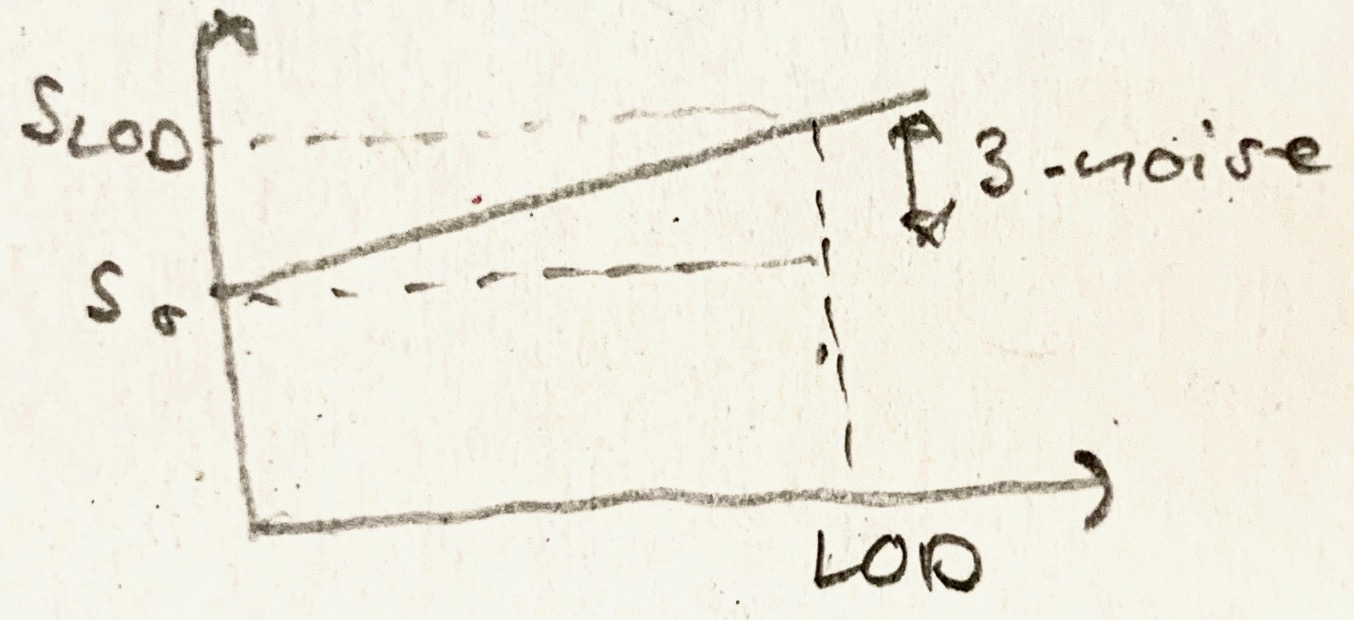
\includegraphics[width=\columnwidth]{Biosensors_LOD}
\end{minipage}

\formbox{LOD for intensity/signal}{LOD_{NSB} = \avg{I_{NSB}} + 3\;\sigma(I_{NSB})}
\formula{Lowest detectable intensity}{\frac{ \avg{I_{POI}} }{ LOD_{NSB} } = 1}
($\!\!~_{POI}$: proteins of interest)
\formula{Detectable \#proteins}{N\!\# = \frac{\Gamma}{m\ped{protein}}} \quad
$[\Gamma] = \unitfrac{pg}{mm^2}$ detection limit

		%! Author = tstreule

\section{Optical Microscopy}
%%%%%%%%%%%%%%%%%%%%%%%%%%%%%%%%%%%%%%%%%%%%%%%%%%%%%%
%%%%%%%%%%%%%%%%%%%%%%%%%%%%%%%%%%%%%%%%%%%%%%%%%%%%%%
\subsection{Reflection and Refraction}
%
\formbox{Law of Reflection}{\theta\ped{inc} = \theta_2}
\formbox{Law of Refraction}{\frac{n\ped{inc}}{n_2} = \frac{\lambda_0/\lambda\ped{inc}}{\lambda_0/\lambda_2} = \frac{\sin\theta_2}{\sin\theta\ped{inc}}}
\quad for $\theta\ped{inc}<\theta_c$
\formula{Total reflection}{\sin\theta_c = n_2/n\ped{inc}}
\quad \textbf{always total} if $n\ped{inc}<n_2$

\formula{Paraxial approx.}{\theta \simeq \sin\theta \simeq \tan\theta, \;\;\; \theta\ll 1}
\formula{Thin lens approx.}{R \ll S_o,\,S_i}
\formbox{Lens makers formula}{\frac{1}{S_o} + \frac{1}{S_i} = \frac{1}{f} = \frac{n_\textrm{lens}-n}{n} \left( \frac{1}{R_1} - \frac{1}{R_2} \right)}
%%%%%%%%%%%%%%%%%%%%%%%%%%%%%%%%%%%%%%%%%%%%%%%%%%%%%%
\subsection{Ray Tracing}
%
%	\begin{itemize}
%		\item Rays passing \textbf{through the optical center} of a lens continue in a straight line
%		\item Rays traveling \textbf{parallel to the optical axis} pass through the focal point after refraction and vice versa
%		\item \textbf{Parallel rays} pass through the same point in the focal plane after refraction and vice versa
%	\end{itemize}
\begin{minipage}{\linewidth}
    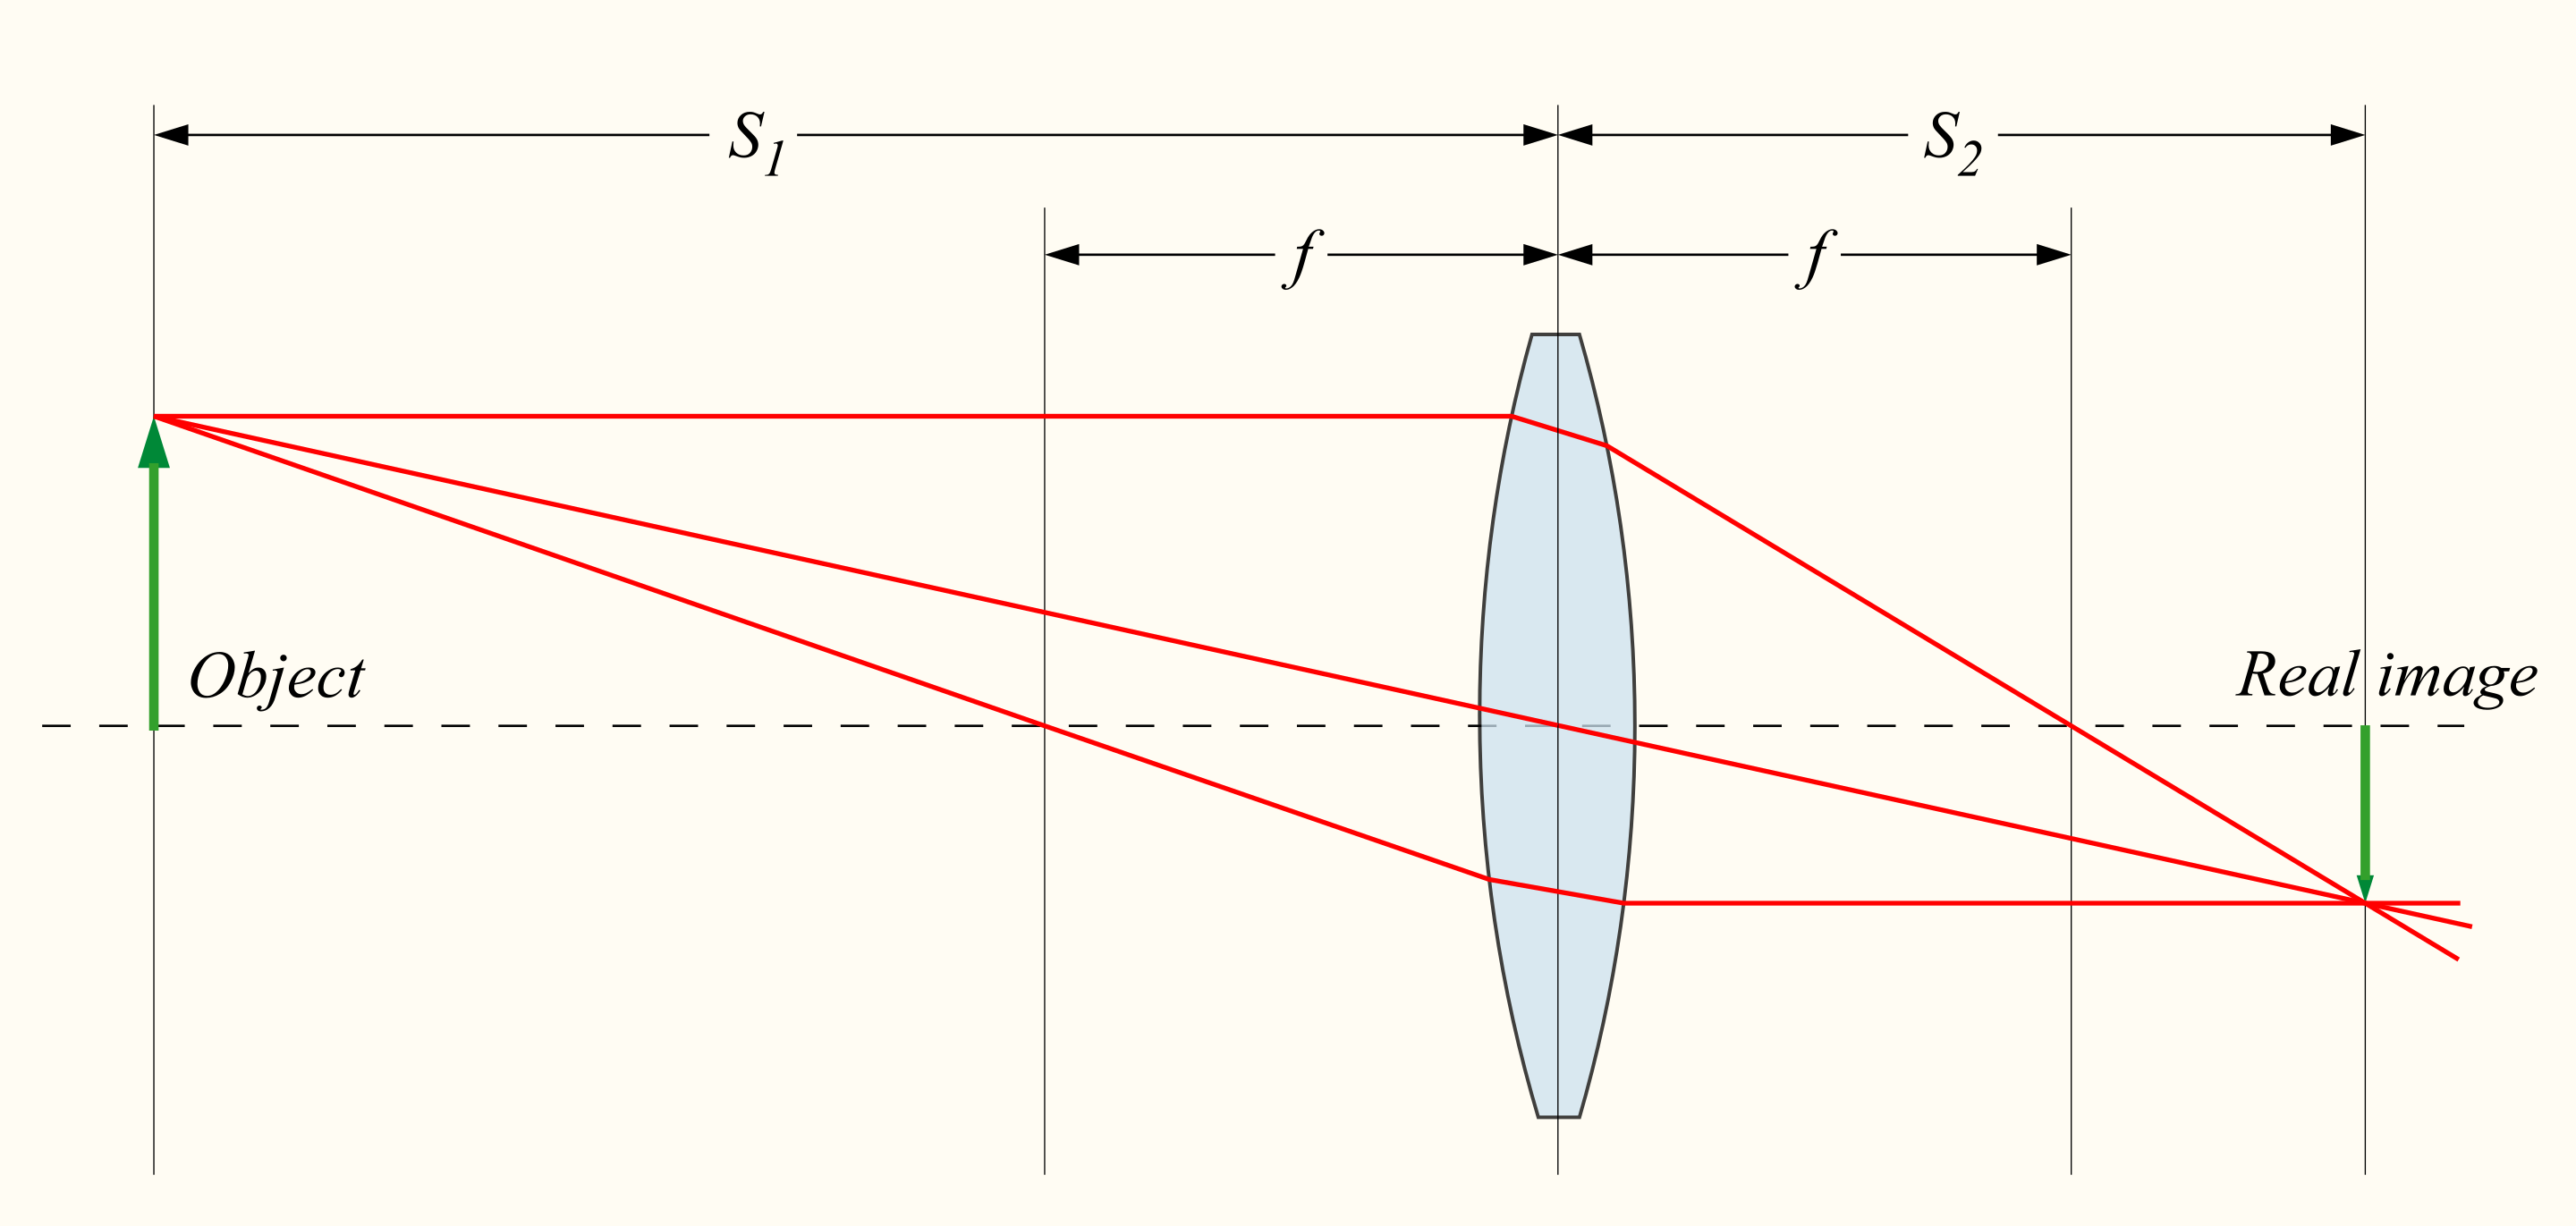
\includegraphics[width=.45\columnwidth]{Optical_Lens}
    \qquad
    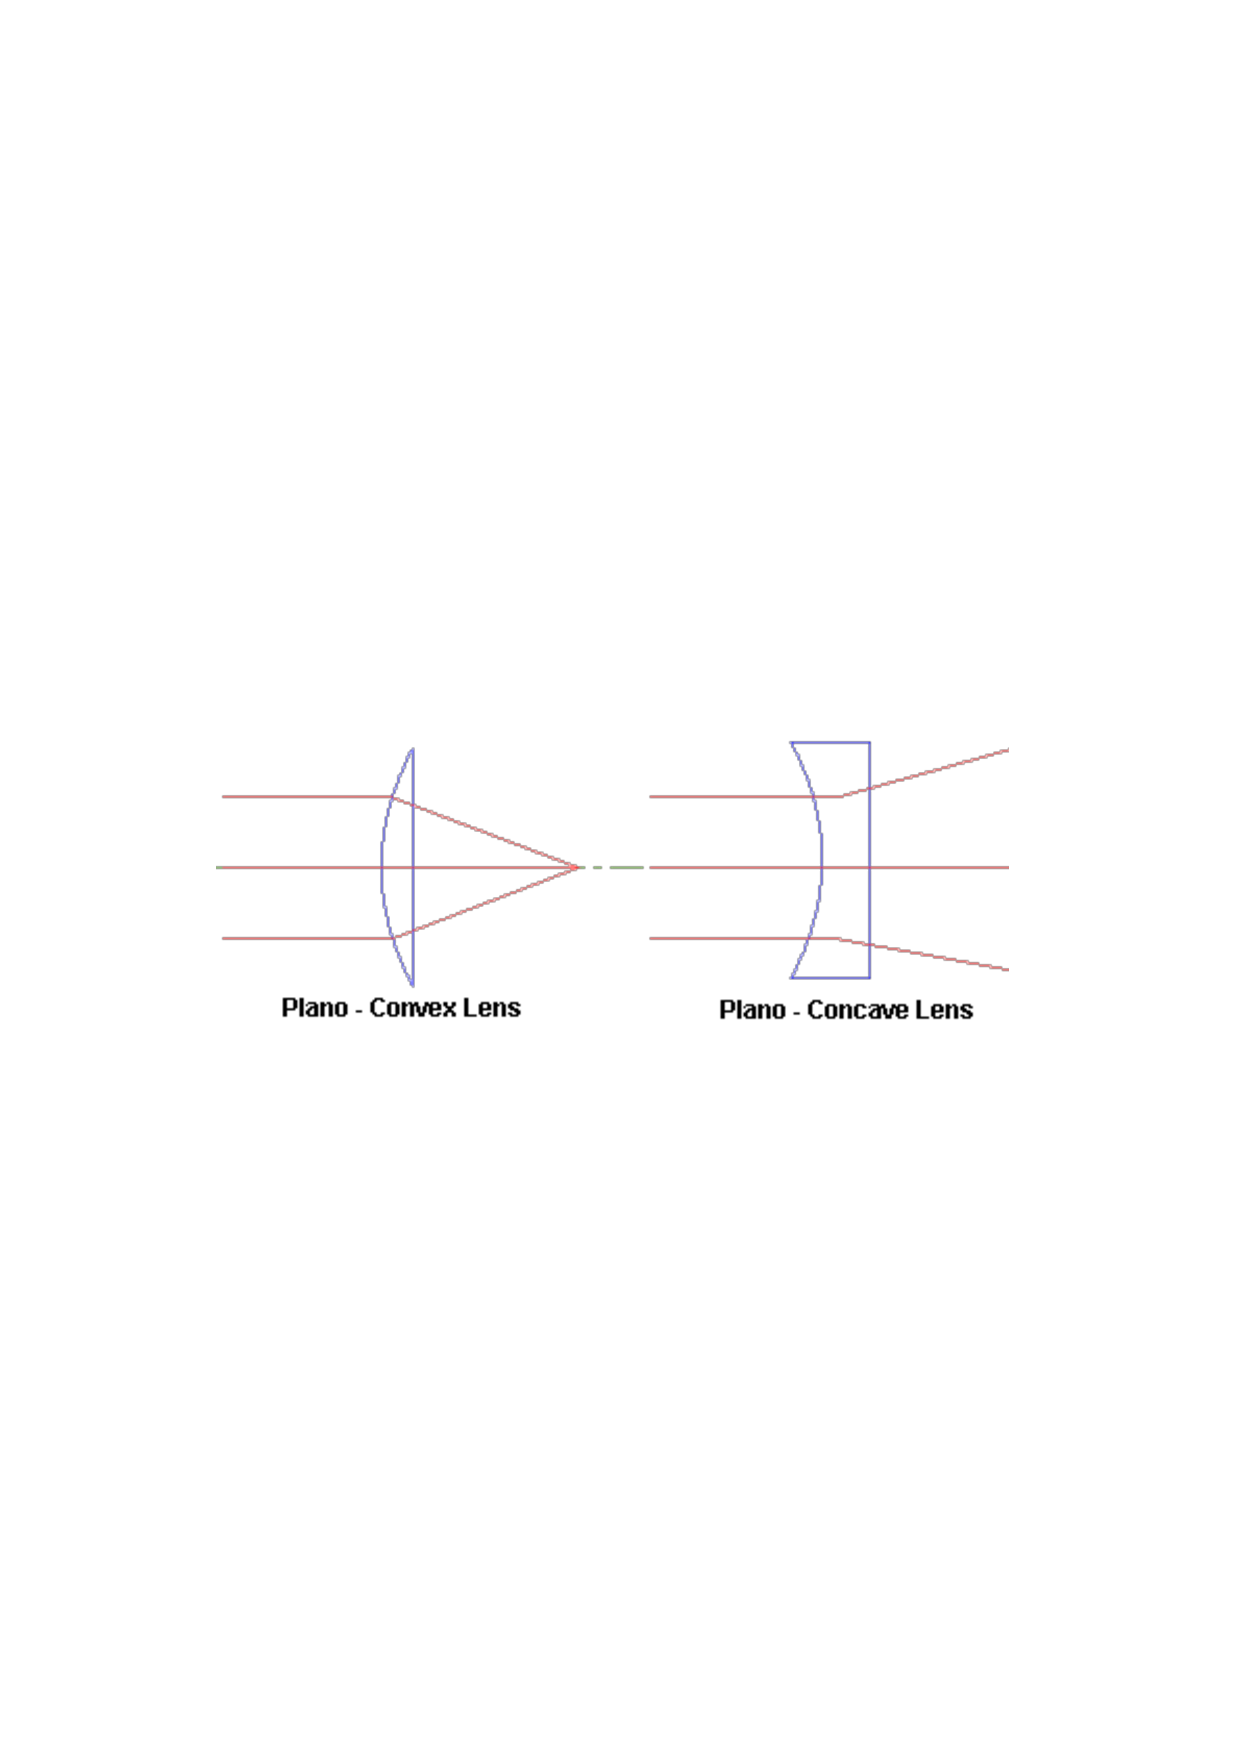
\includegraphics[width=.4\columnwidth]{Optical_Lens2}
\end{minipage}
%%%%%%%%%%%%%%%%%%%%%%%%%%%%%%%%%%%%%%%%%%%%%%%%%%%%%%
\begin{minipage}{\linewidth}
    \begin{minipage}[t]{.5\columnwidth-.5\columnsep}
        \subsubsection{Simple Microscope}
        %
        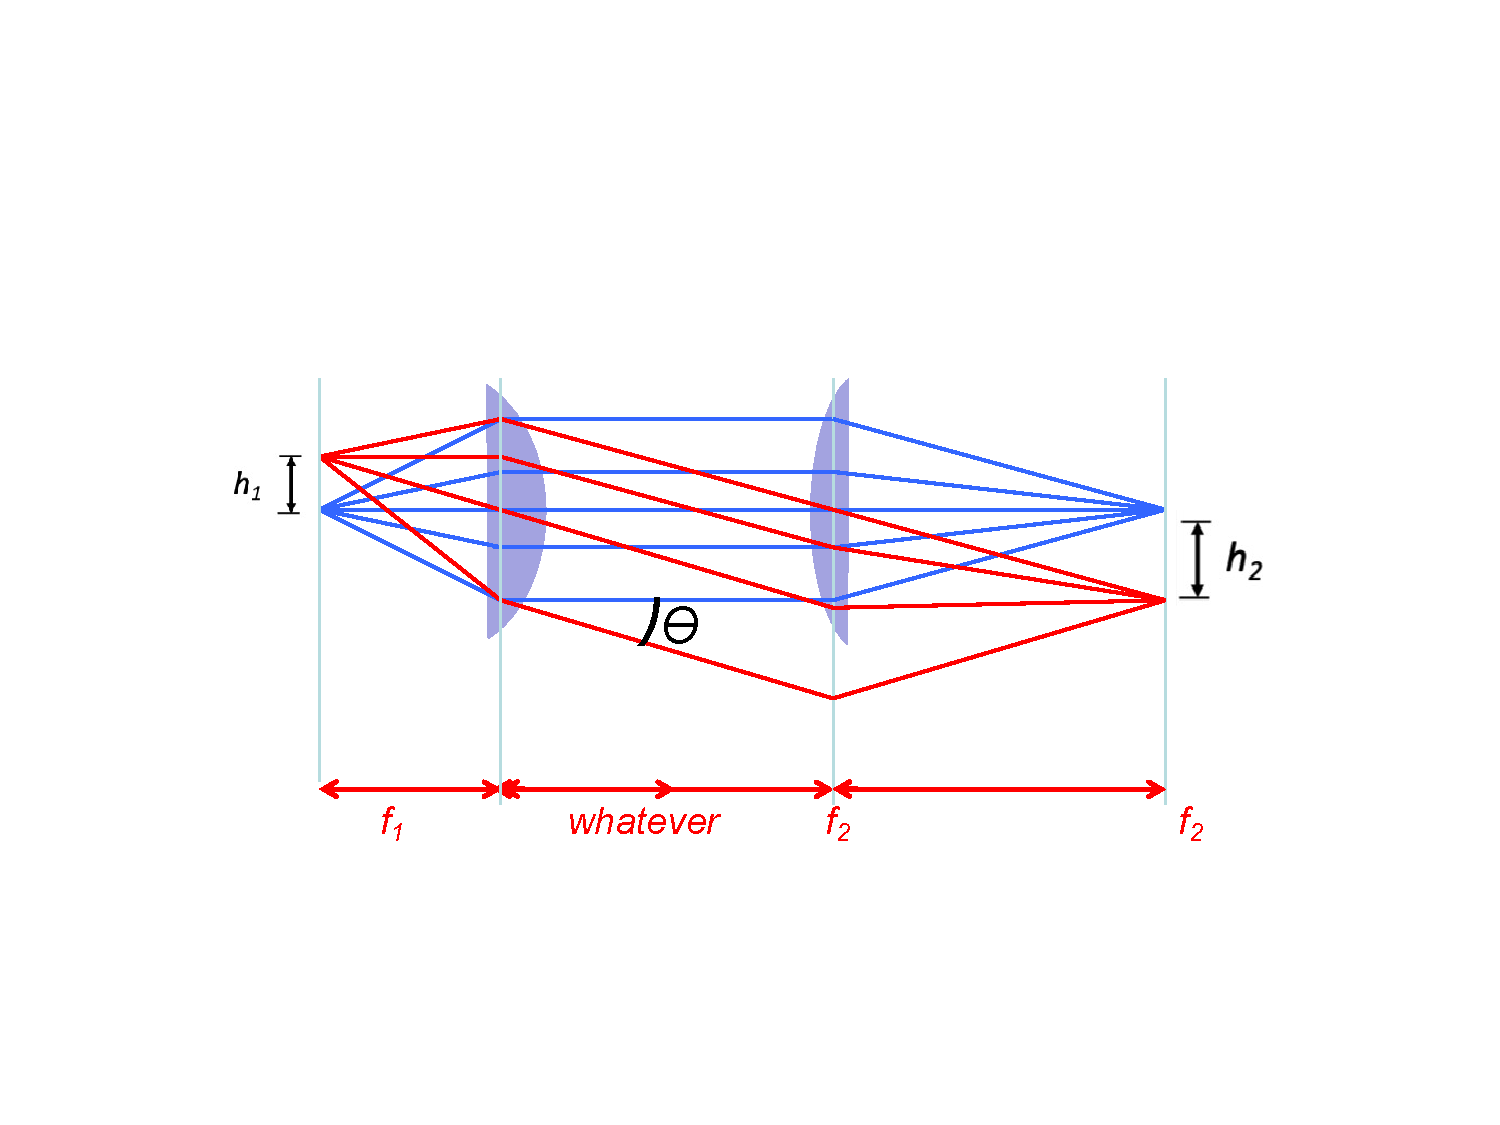
\includegraphics[width=\columnwidth]{Optical_Simple_Microscope}
    \end{minipage}%
    \hspace{\columnsep}%
    \begin{minipage}[t]{.5\columnwidth-.5\columnsep}
        \subsubsection{Beam Expander}
        %
        \hfill for light source

        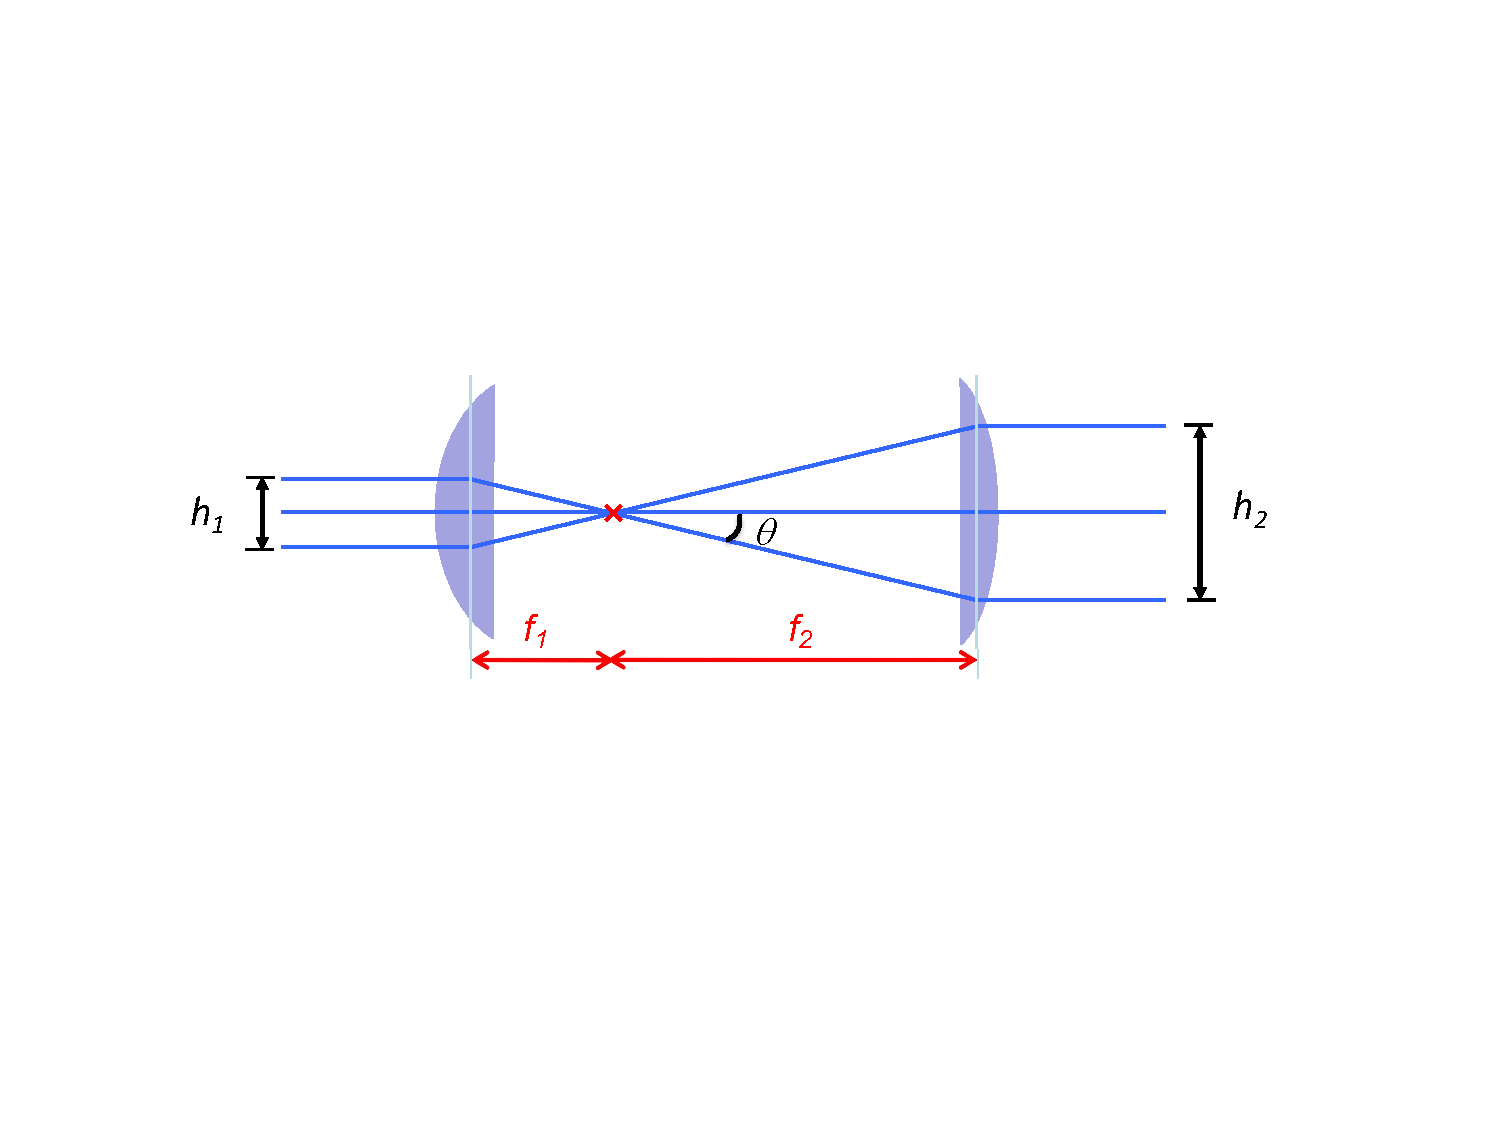
\includegraphics[width=\columnwidth]{Optical_Beam_Expander}
    \end{minipage}

    \formbox{Magnification}{M = h_2/h_1 \overset{*}{=} f_2/f_1}
    \quad * since $h_1 = f_1\sin\theta$
\end{minipage}
%%%%%%%%%%%%%%%%%%%%%%%%%%%%%%%%%%%%%%%%%%%%%%%%%%%%%%
\subsubsection{Simple ``modern'' Microscope}
%
\parbox{.5\columnwidth}{(uniform!) Illumination:}
\parbox{.5\columnwidth}{Camera: ($M = f_{tube} / f_{obj}$)}

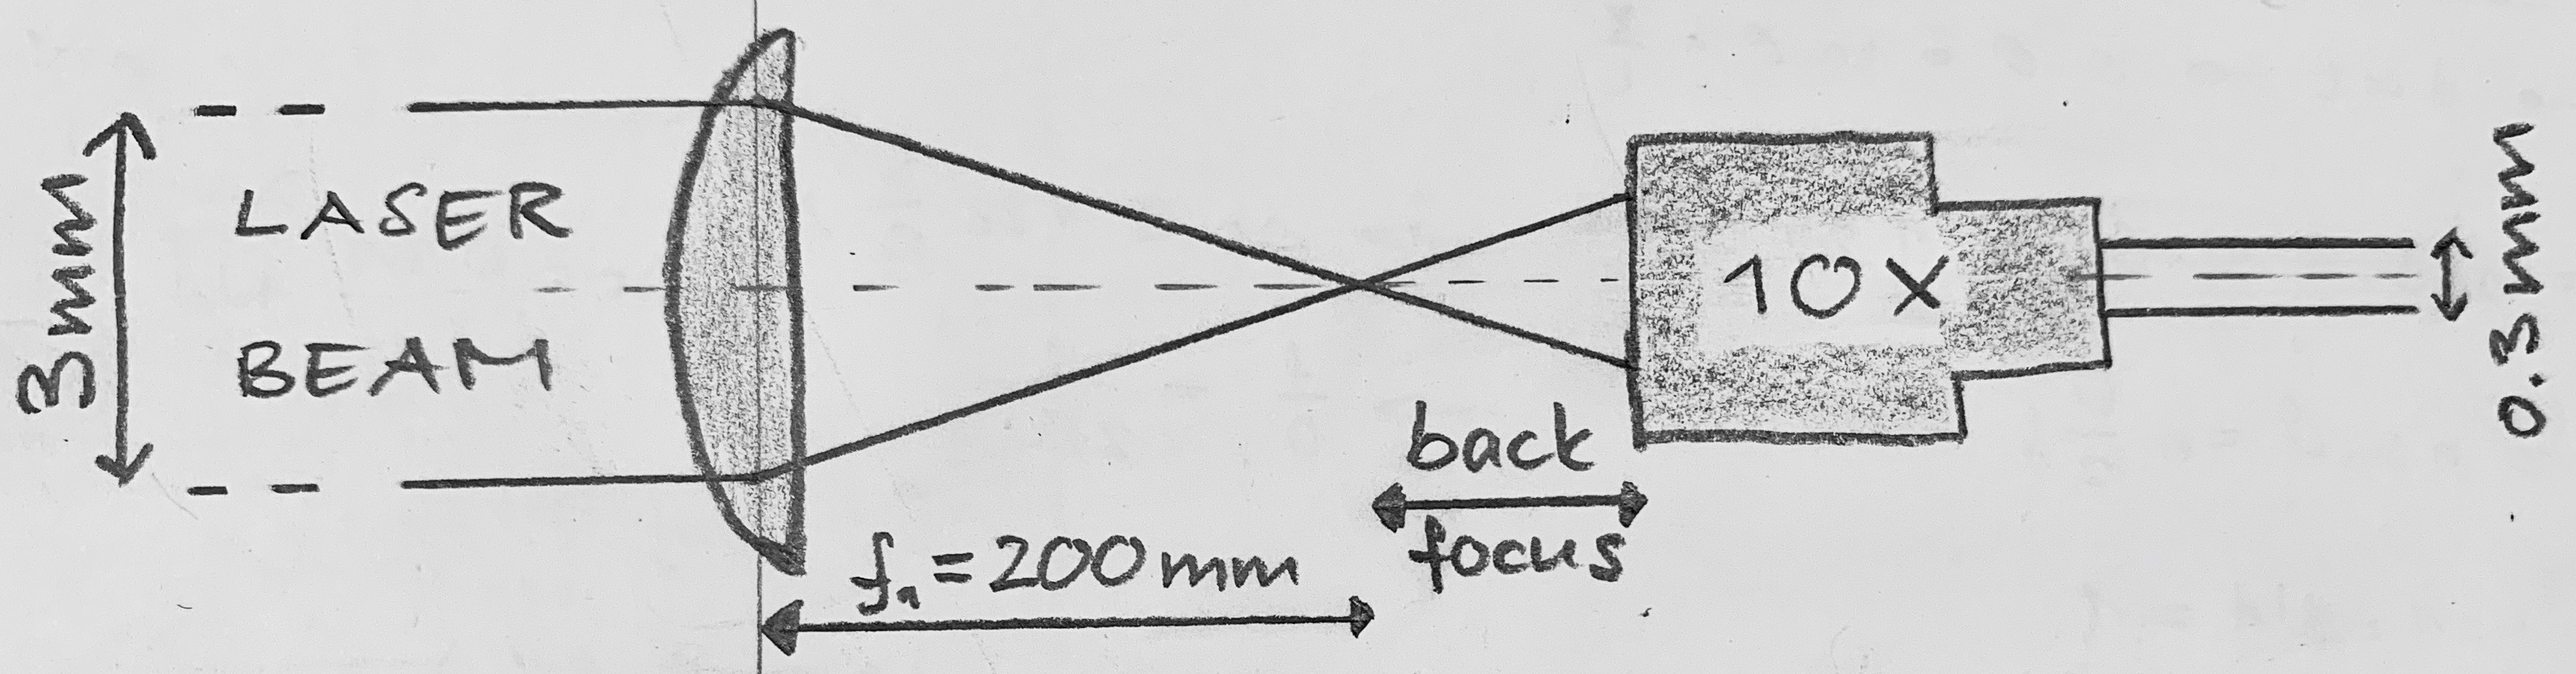
\includegraphics[width=.49\columnwidth]{Optical_Modern_Illumination}
\hfill
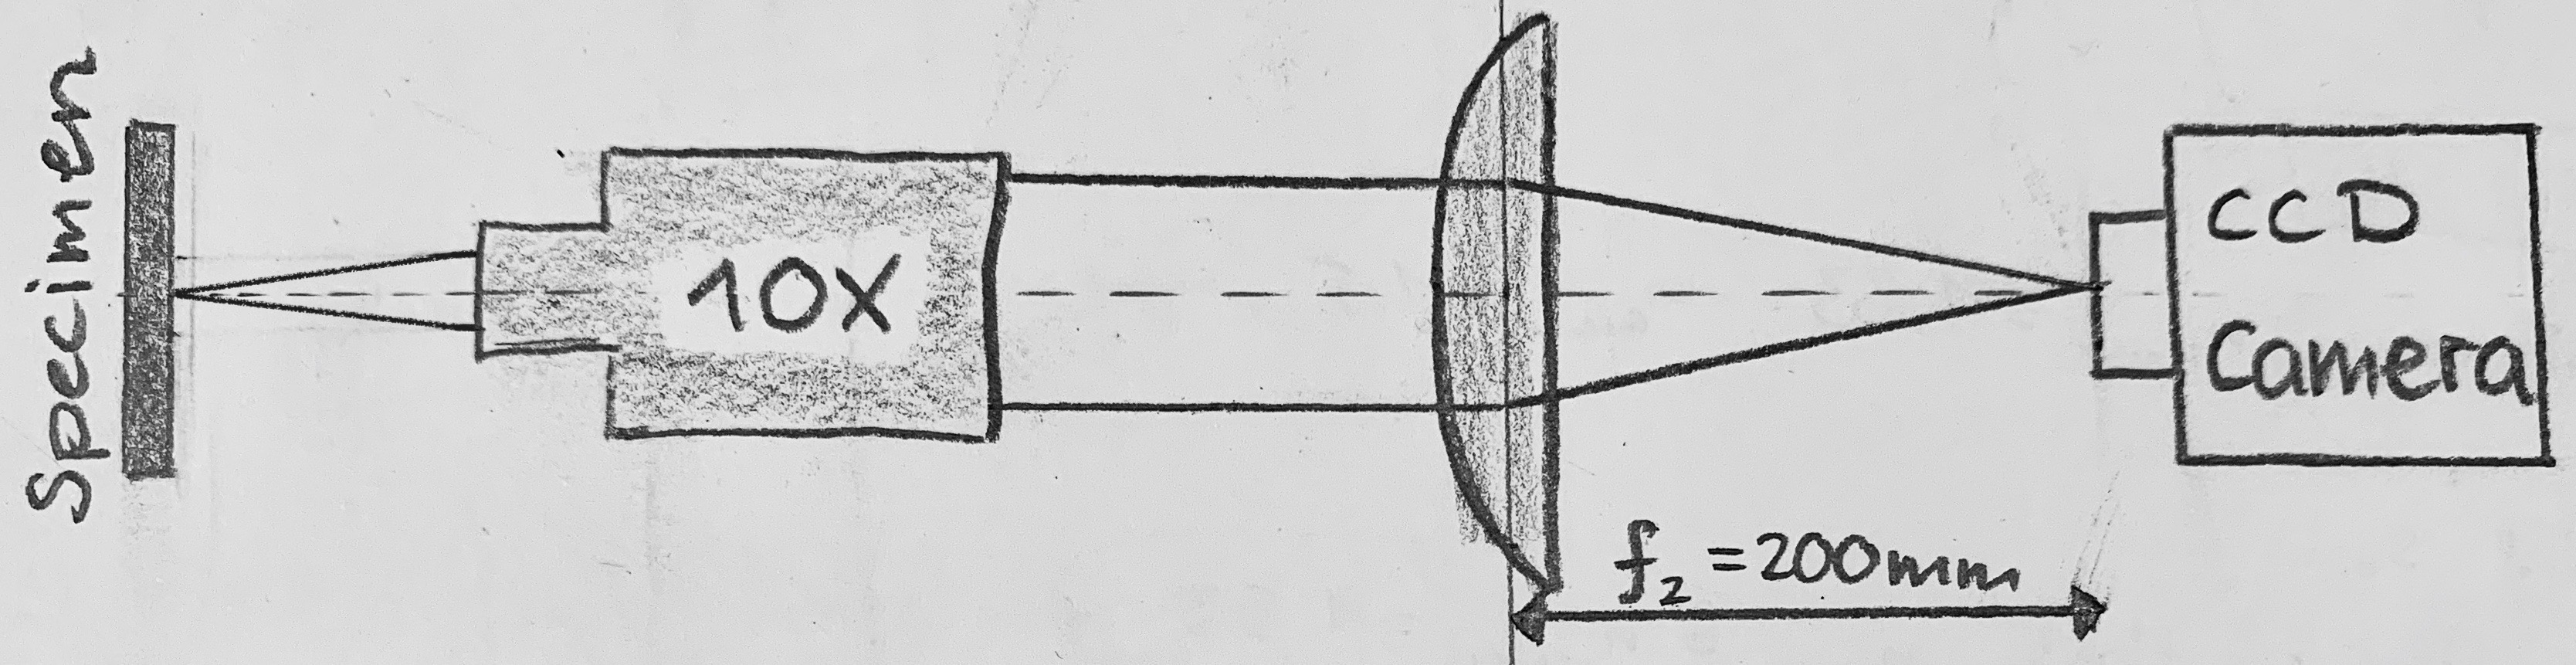
\includegraphics[width=.49\columnwidth]{Optical_Modern_Camera}

\parbox{.5\columnwidth}{\centering\small(Objective lens)}
\parbox{.5\columnwidth}{\centering\small(Tube lens)}
%%%%%%%%%%%%%%%%%%%%%%%%%%%%%%%%%%%%%%%%%%%%%%%%%%%%%%
\subsection{Fundamental Limits of Lenses \& Resulution}
%
Due to a \textbf{finite aperture} will points presented as the PSF (point-spread).

\begin{minipage}{.3\columnwidth}
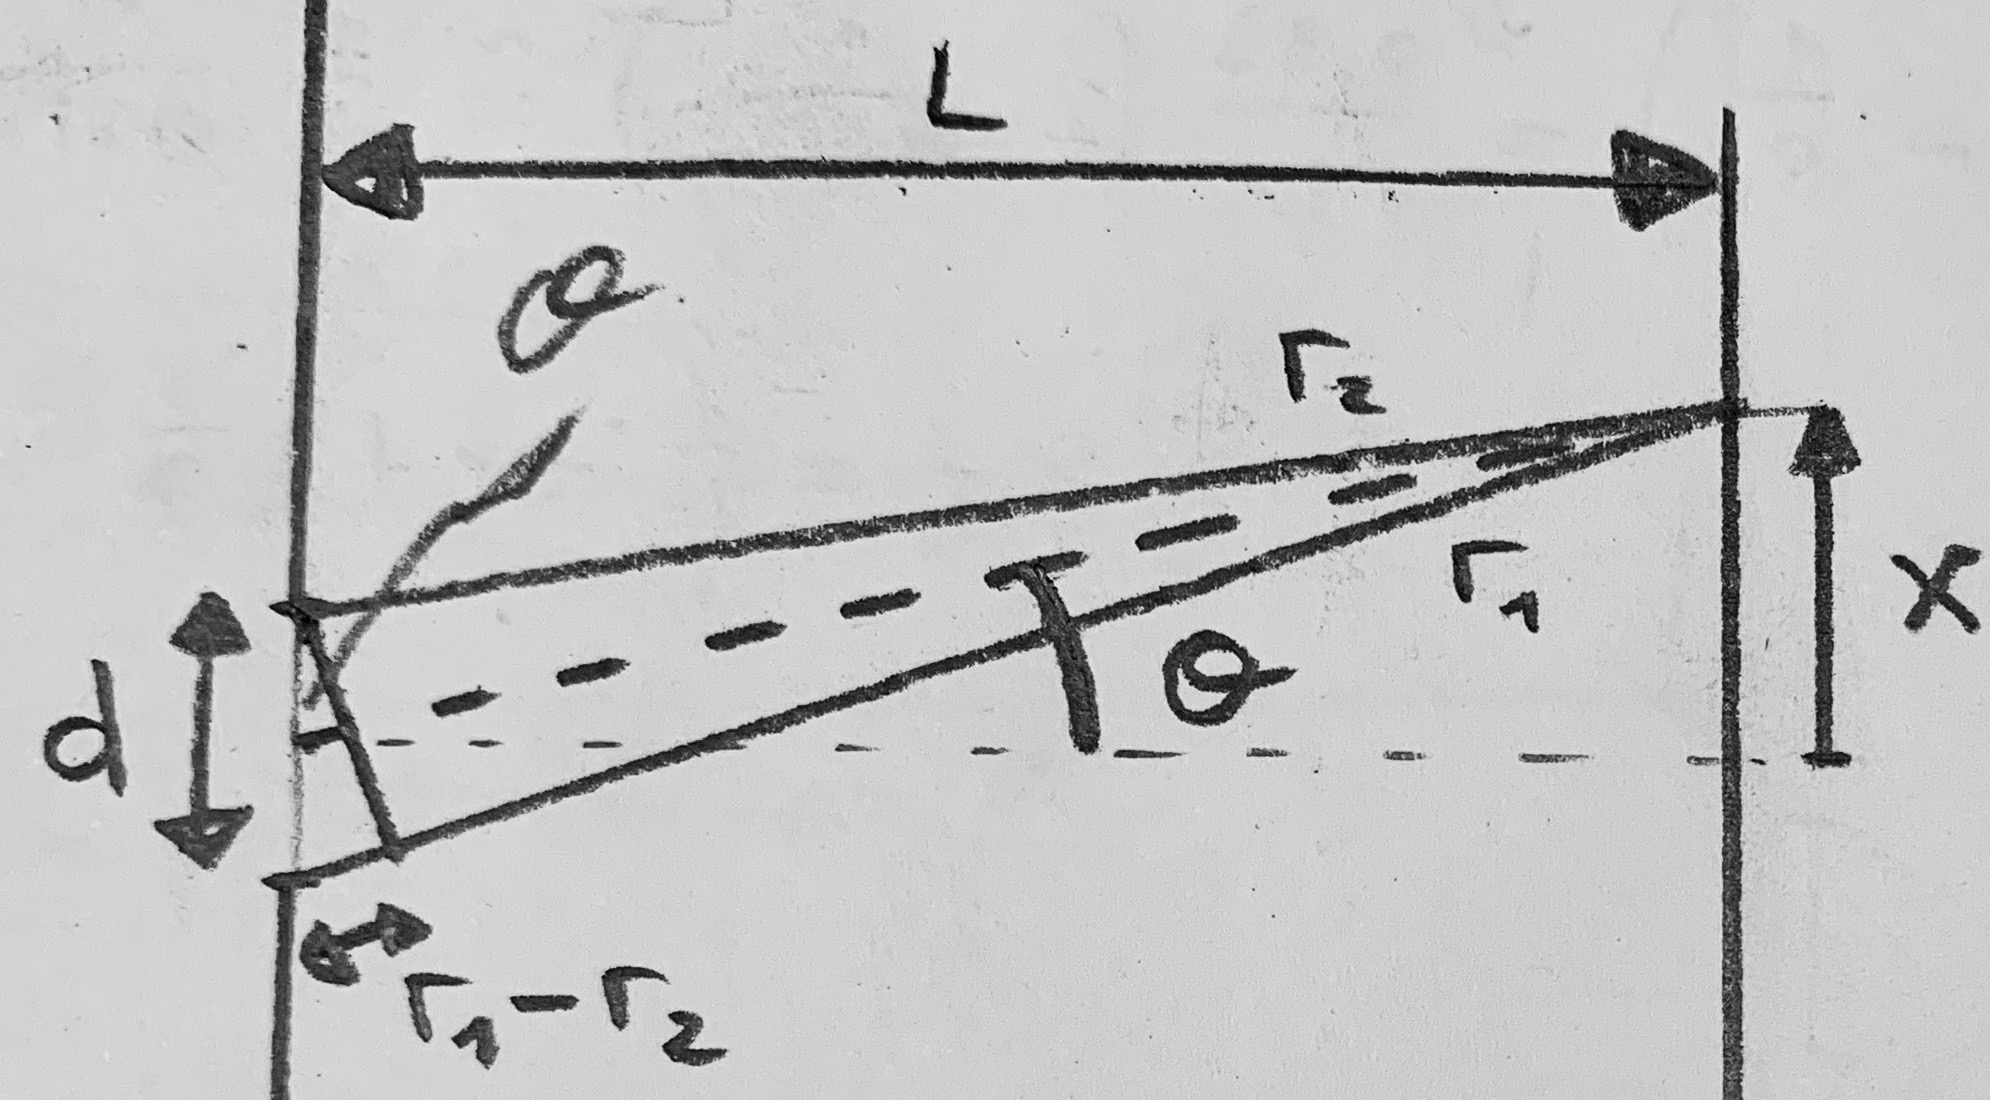
\includegraphics[width=\columnwidth]{Optical_PSF}
\end{minipage}%
\hspace{1.5\boxmargin}%
\begin{minipage}{.7\columnwidth-1.5\boxmargin}
First zero occurs at: \quad
$\theta \overset{(\theta\ll1)}{\simeq} \sin\theta \simeq 1.22\frac{\lambda_0}{d}$\\
$d$: radius of the aperture\par
$\bullet$ $\sin\theta \simeq \tan\theta = x/L$\\
$\bullet$ $r_1 - r_2 = d\cdot x/L$
\end{minipage}

\formtex{\textbf{Rayleigh criterion}}{maximum of the one is on the minimum of the}
\formtex{~}{other curve (FWHM)}
\formbox{Resolution}{\Delta r \simeq f\sin\theta \times M \simeq 1.22\frac{\lambda_0f}{D} \times M = 0.61\frac{\lambda_0n}{\textrm{NA}} \times M \vspace{-1mm}}
\formbox{Numerical Aperture}{\textrm{NA} = n\sin\theta \simeq n\,\frac{D}{2f}}
\quad $n$: refractive index,
\formula{~}{\text{$D$: aperture size of lens, $f$: focal length of lens}}
%%%%%%%%%%%%%%%%%%%%%%%%%%%%%%%%%%%%%%%%%%%%%%%%%%%%%%
\subsection{Fluorescence Microscopy}
%
Emitted photon has \textbf{less energy}.
$\to$ Absorption $\neq$ emission spectr.

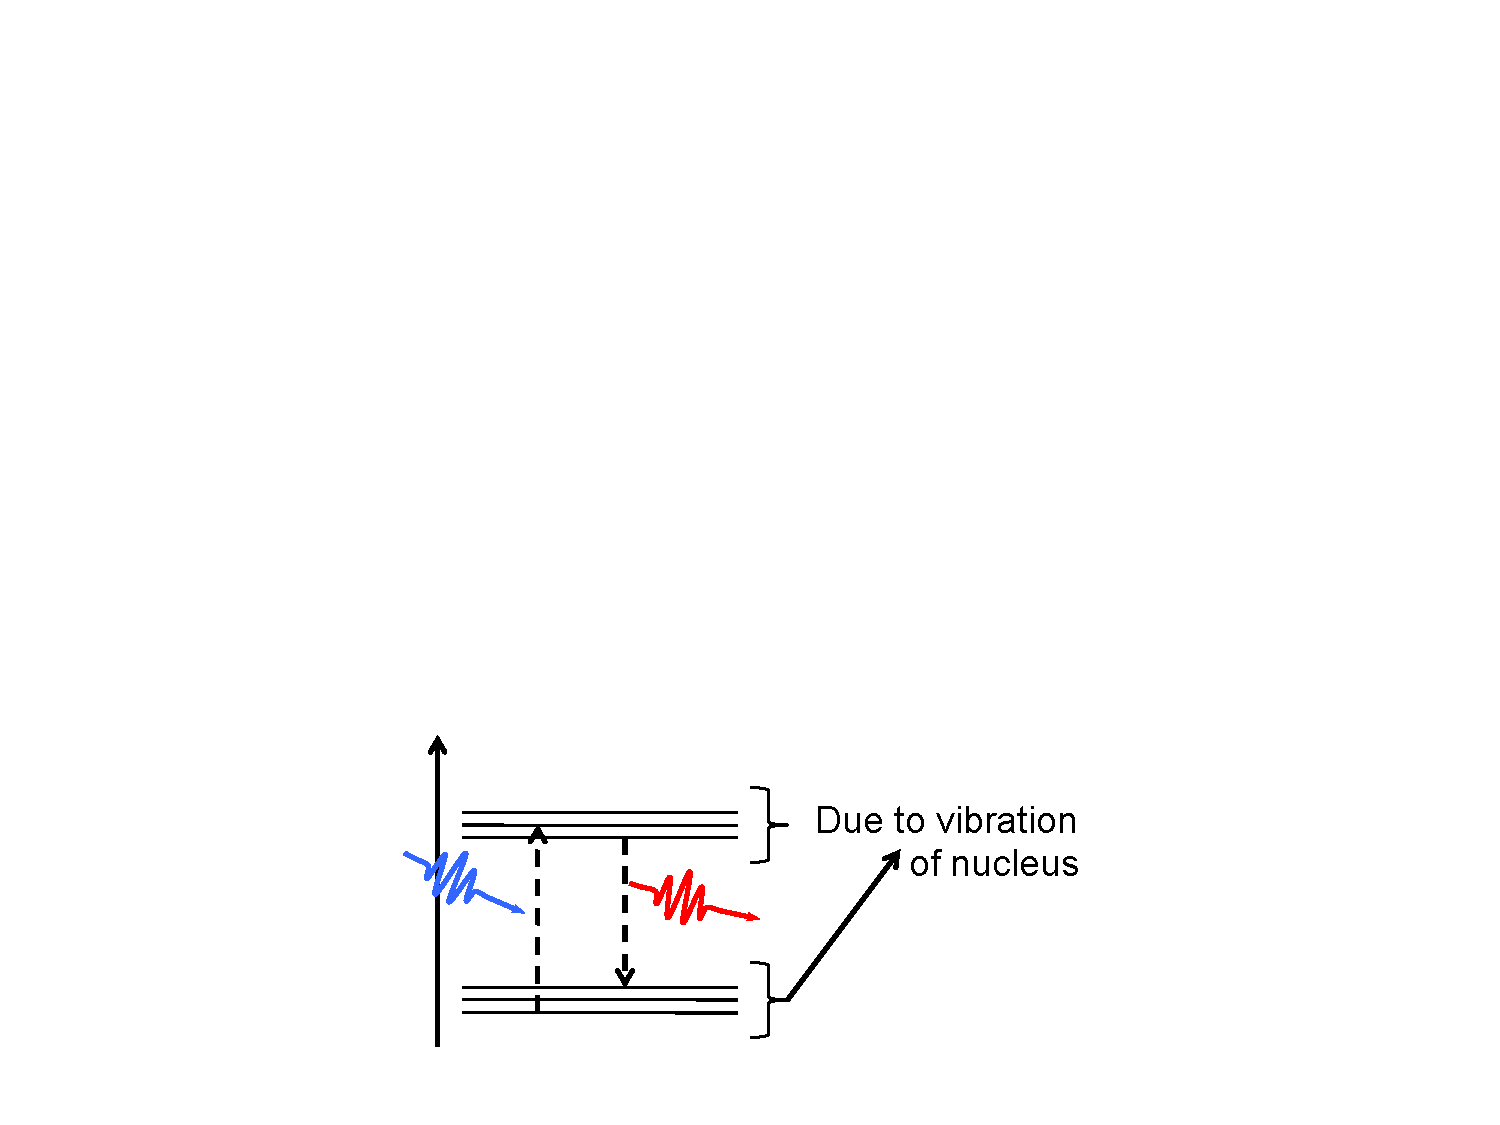
\includegraphics[width=.5\columnwidth]{Optical_Excitation_Emission}
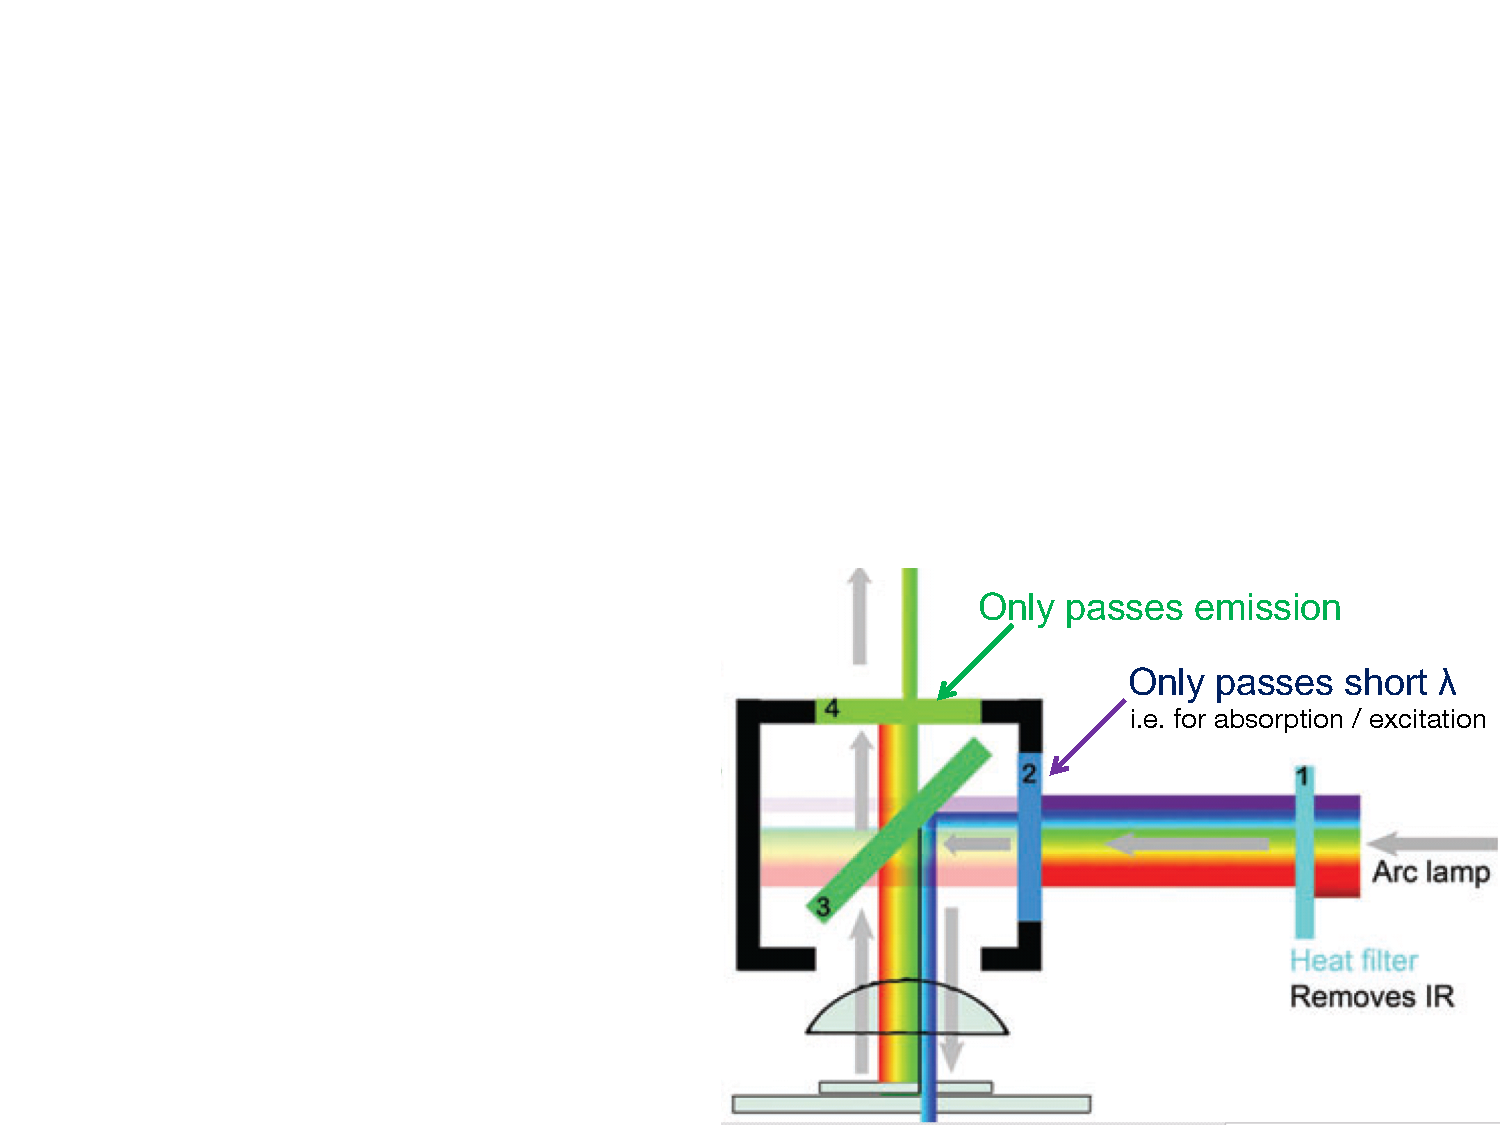
\includegraphics[width=.5\columnwidth]{Optical_Fluorescence_Setup}

		%! Author = tstreule

\section{Mechanical Sensors}
%%%%%%%%%%%%%%%%%%%%%%%%%%%%%%%%%%%%%%%%%%%%%%%%%%%%%%
%%%%%%%%%%%%%%%%%%%%%%%%%%%%%%%%%%%%%%%%%%%%%%%%%%%%%%
\subsection{Viscoelastic media}
%
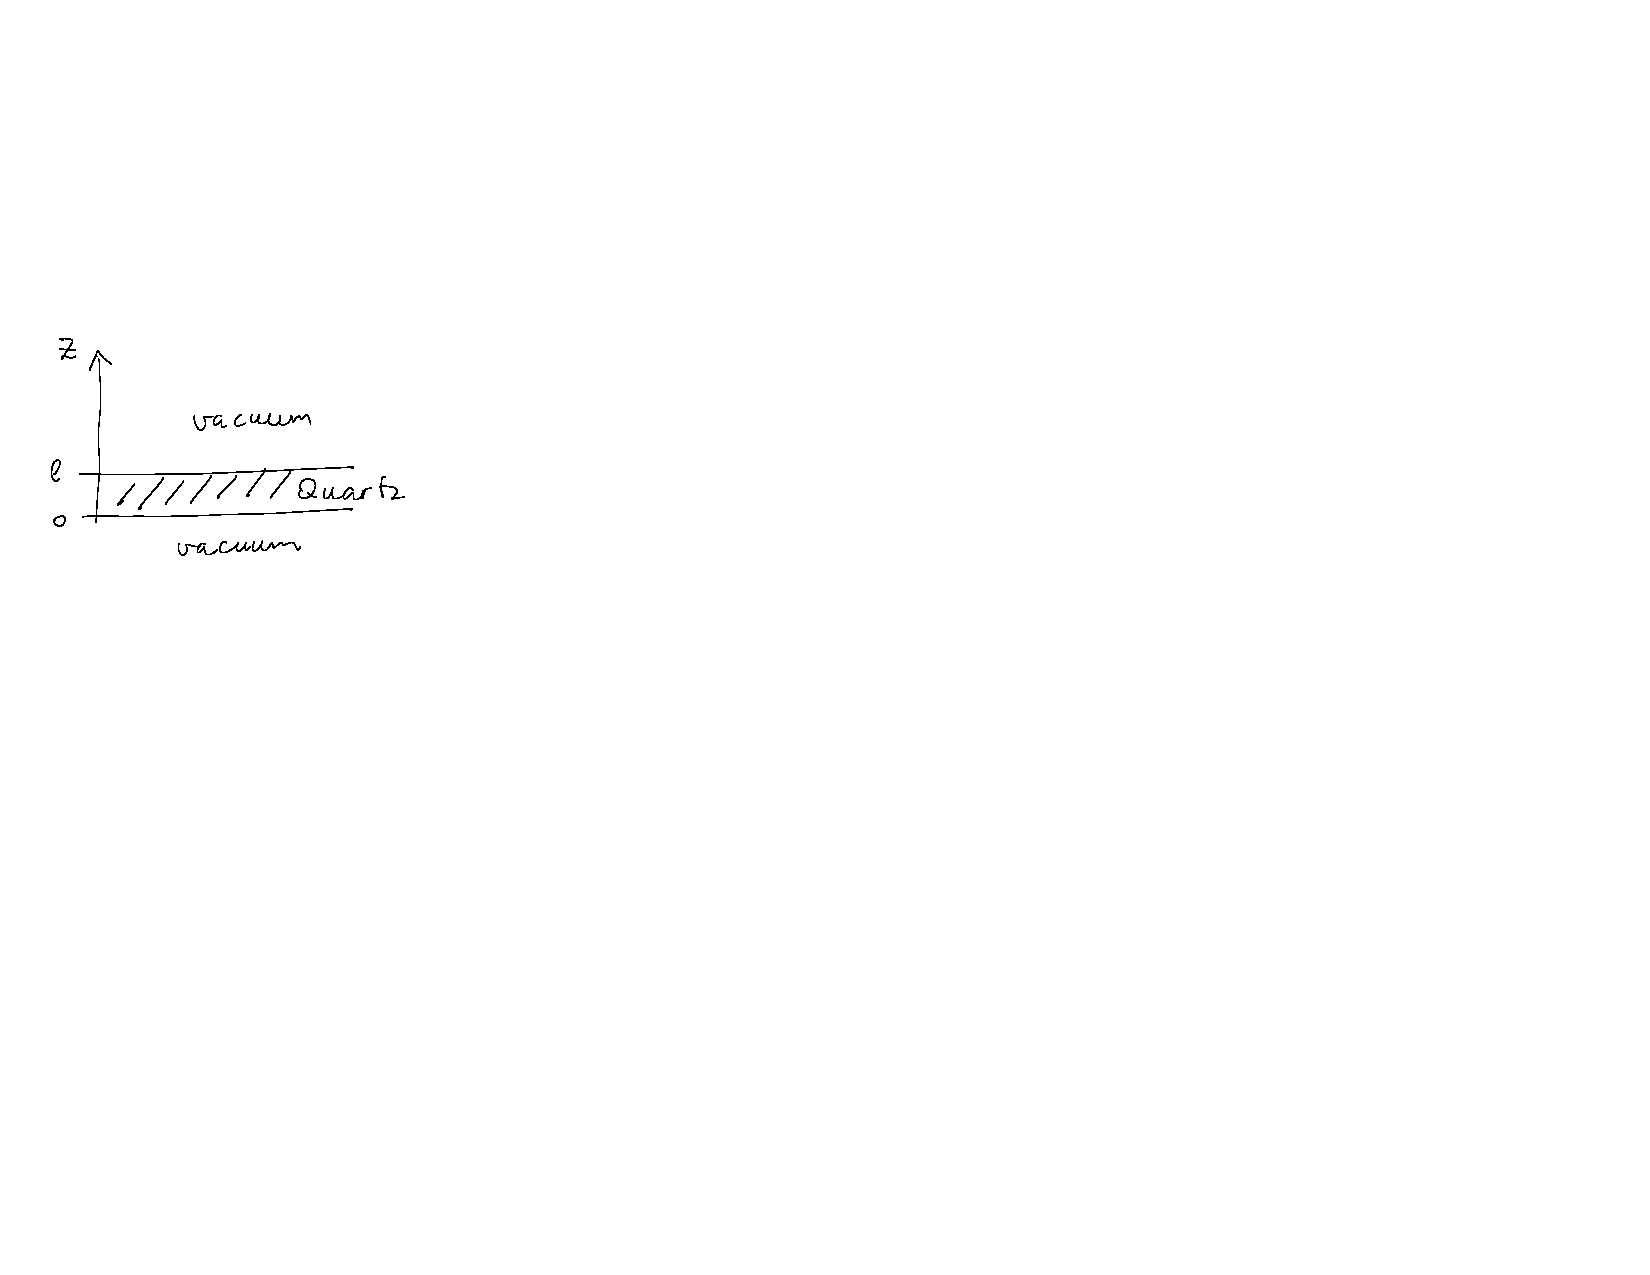
\includegraphics[width=.3\columnwidth]{Mechanical_1}\hfill
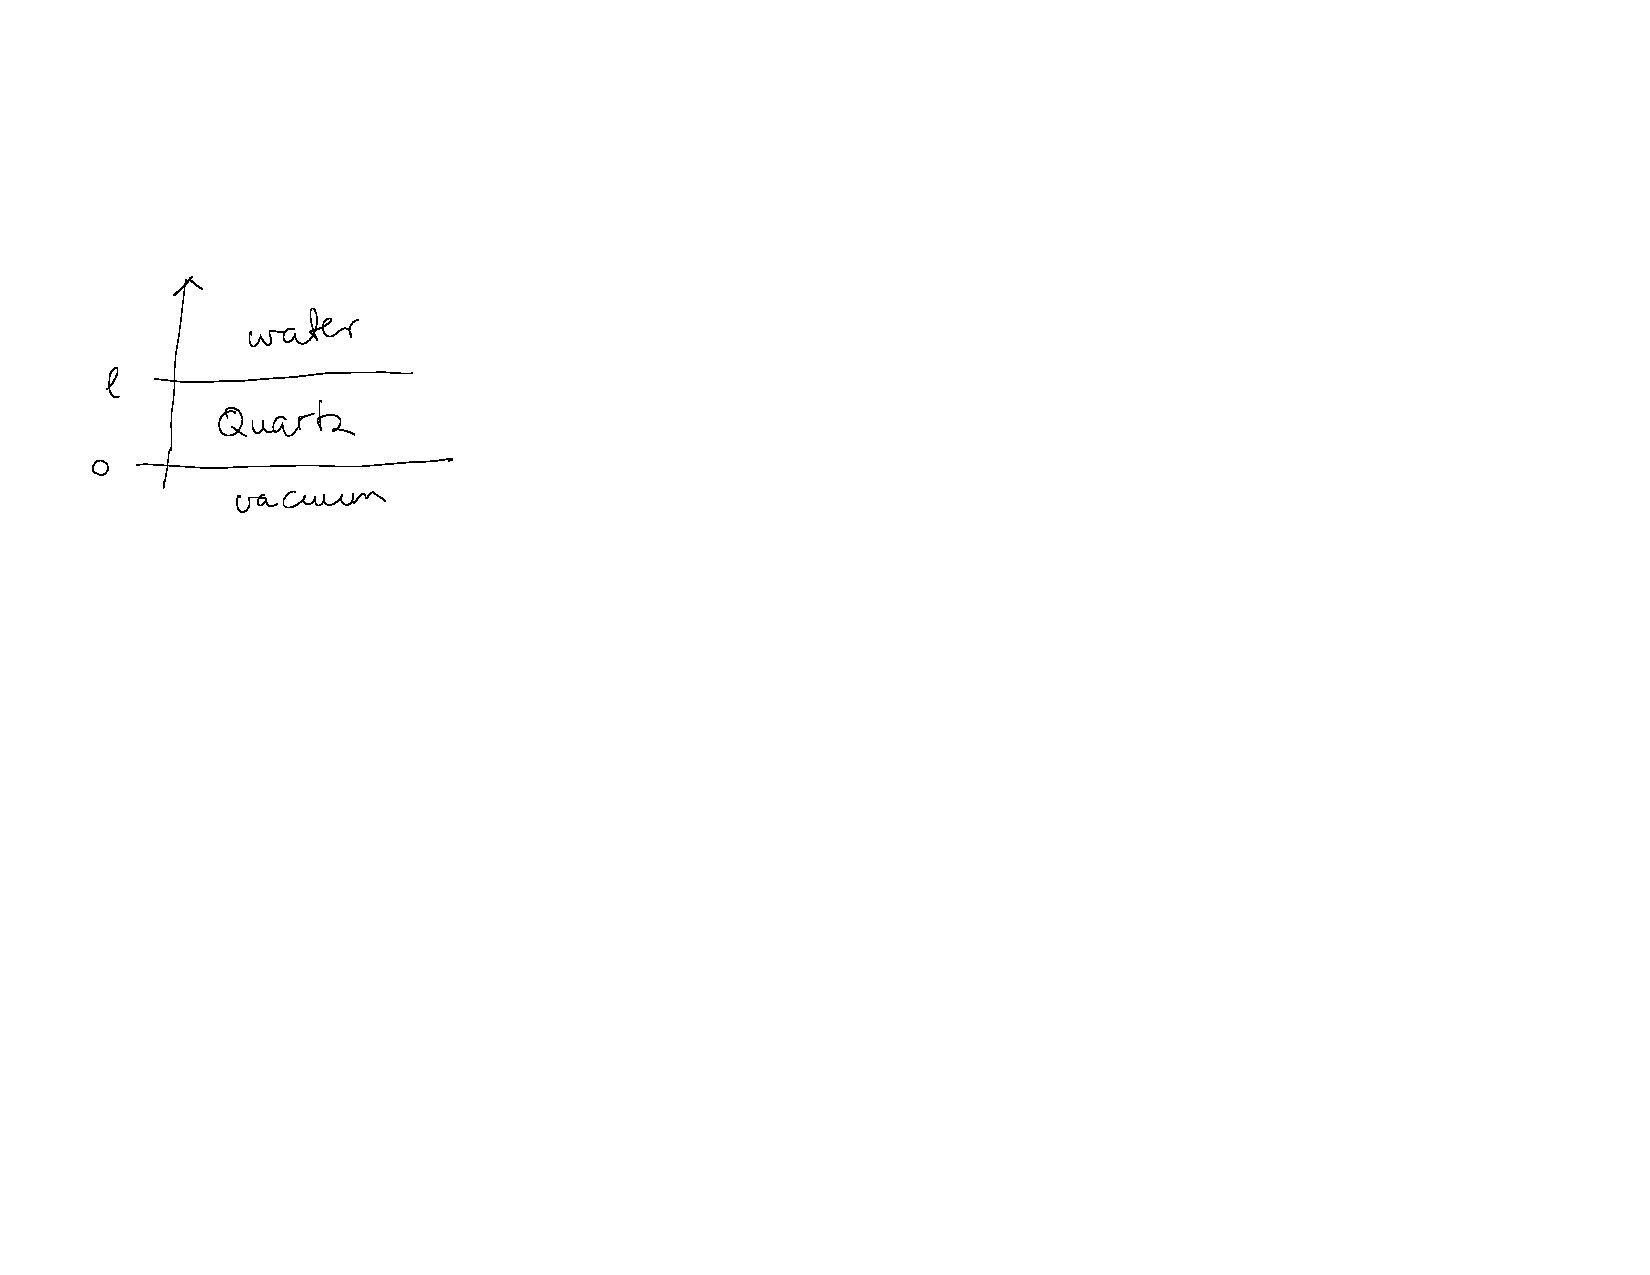
\includegraphics[width=.3\columnwidth]{Mechanical_2}\hfill
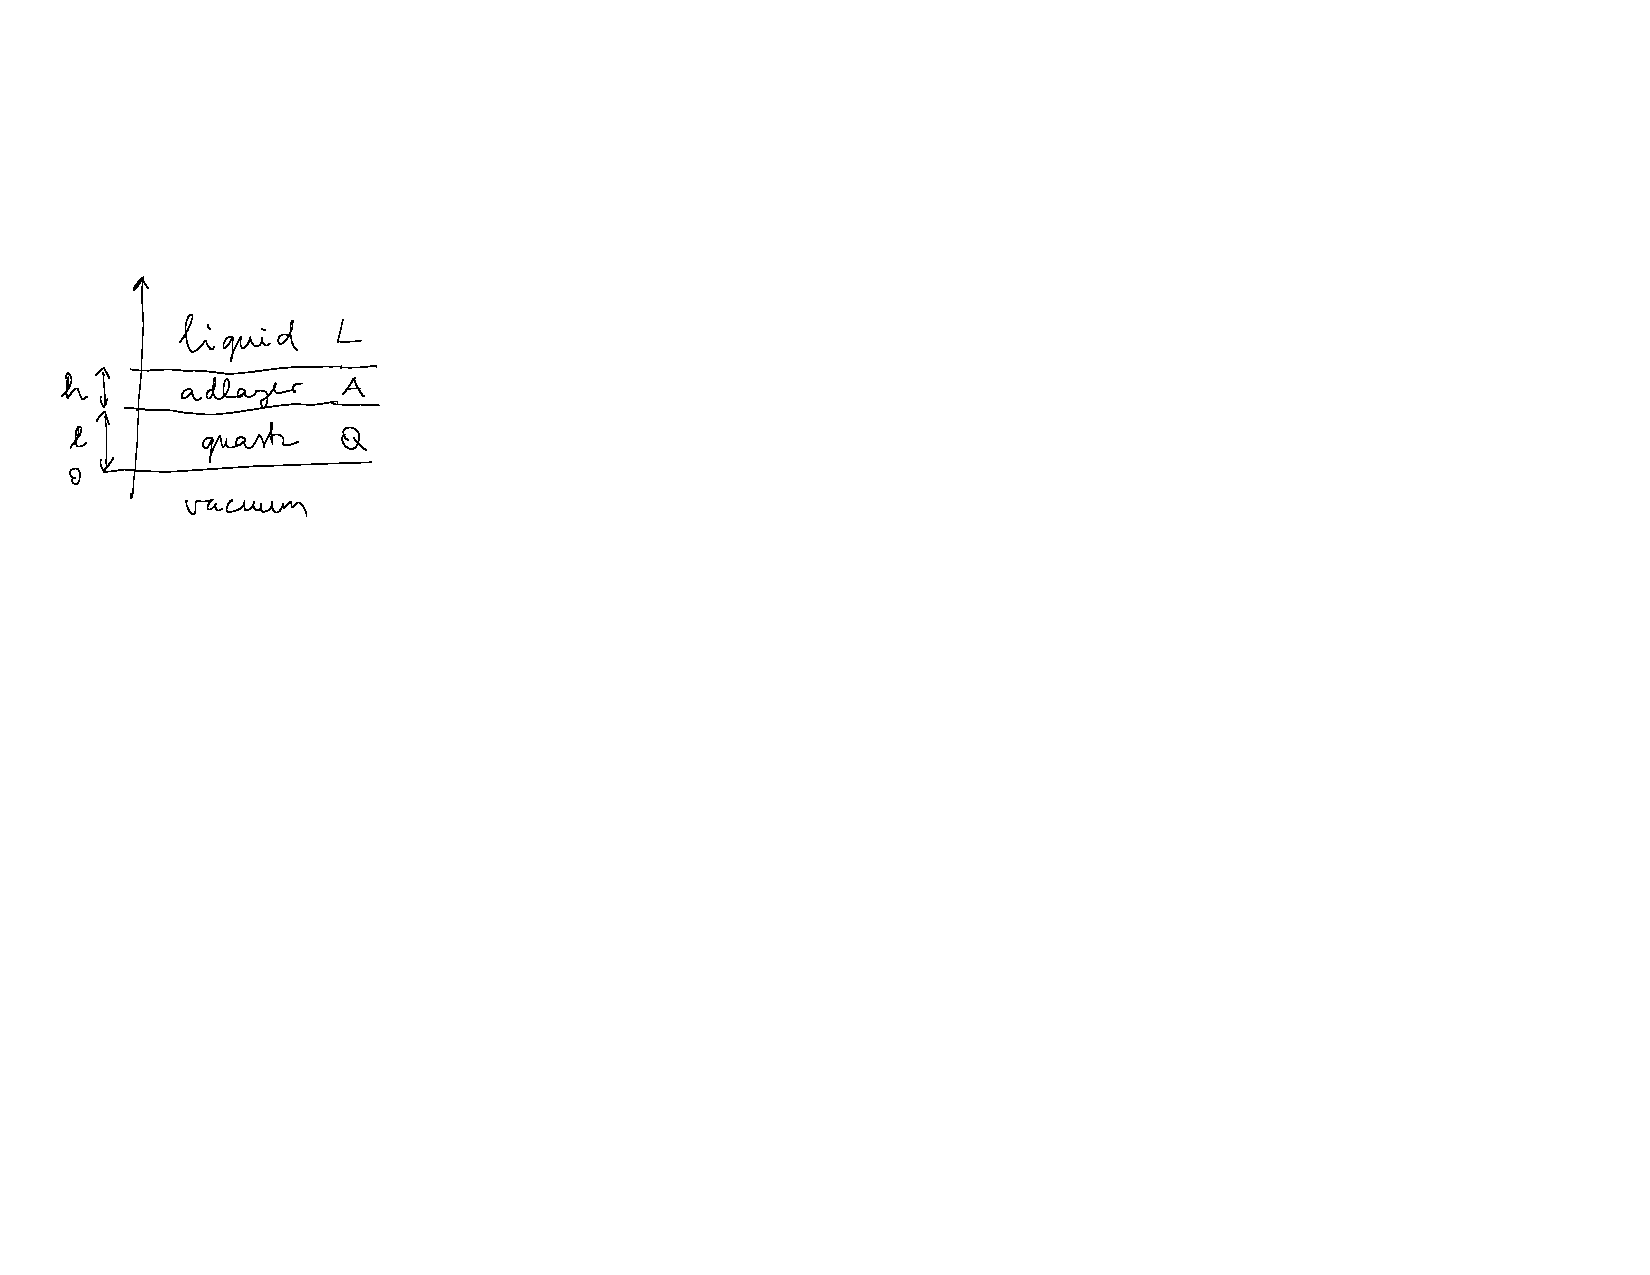
\includegraphics[width=.3\columnwidth]{Mechanical_3}

\textbf{Remark}: Calculate \textit{always} at first in $\unitfrac{rad}{s} \overset{\scriptstyle \times\unitfrac{1}{2\pi}}{\longrightarrow} \unit{Hz}$.
%%%%%%%%%%%%%%%%%%%%%%%%%%%%%%%%%%%%%%%%%%%%%%%%%%%%%%
\subsubsection{Crystal with thickness $l$}
%
\formbox[\unitfrac{rad}{s}]{Resonance frequency}{\omega_n = n\cdot\omega_0 = n\cdot \frac{\pi}{l} \sqrt{\frac{\mu_Q}{\rho_Q}}}
%\formula{overtones}{q\coloneqq \omega\sqrt{\frac{\rho}{\mu}}, \enskip \lambda = 2\pi / q = 2l / n}
\formula{char. wavelength}{\lambda = 2l/n}
%%%%%%%%%%%%%%%%%%%%%%%%%%%%%%%%%%%%%%%%%%%%%%%%%%%%%%
\subsubsection{Elastic plate in water}
%
\formbox{Resonance frequency}{\omega_n = n\omega_0 + \Delta\omega_n}
\formula{frequency shift}{\Delta\omega_n = -\sqrt{n} \,\sqrt{\frac{\rho_L\,\eta_L\,\omega_0}{2}} \frac{1}{l\,\rho_Q} \textrm{,\enskip $\eta_L$: viscosity}}
%%%%%%%%%%%%%%%%%%%%%%%%%%%%%%%%%%%%%%%%%%%%%%%%%%%%%%
\subsubsection{Elastic plate in water with adlayer}
%
In fact is the \textit{resonance frequency} dependent on the adlayer height.\\
But if it is ``enough'' small, the Sauerbrey approx. is sufficient.

\formbox{\textbf{Sauerbrey eq.}}{\!\!\Delta f_n = 2\pi\omega_n = -n\frac{\Delta m}{C}\!\!}
\hfill $C {=}\frac{\sqrt{\rho_Q\,\mu_Q}}{2f_0^2} {=} \unit[17.7]{\!\!\frac{\unit[]{ng}}{\unit[]{cm^2Hz}}}$
%%%%%%%%%%%%%%%%%%%%%%%%%%%%%%%%%%%%%%%%%%%%%%%%%%%%%%
\subsection{QCM-D \textit{vs.} SPR techniques}
%
\begin{tabular}{@{}l @{\qquad}l}
    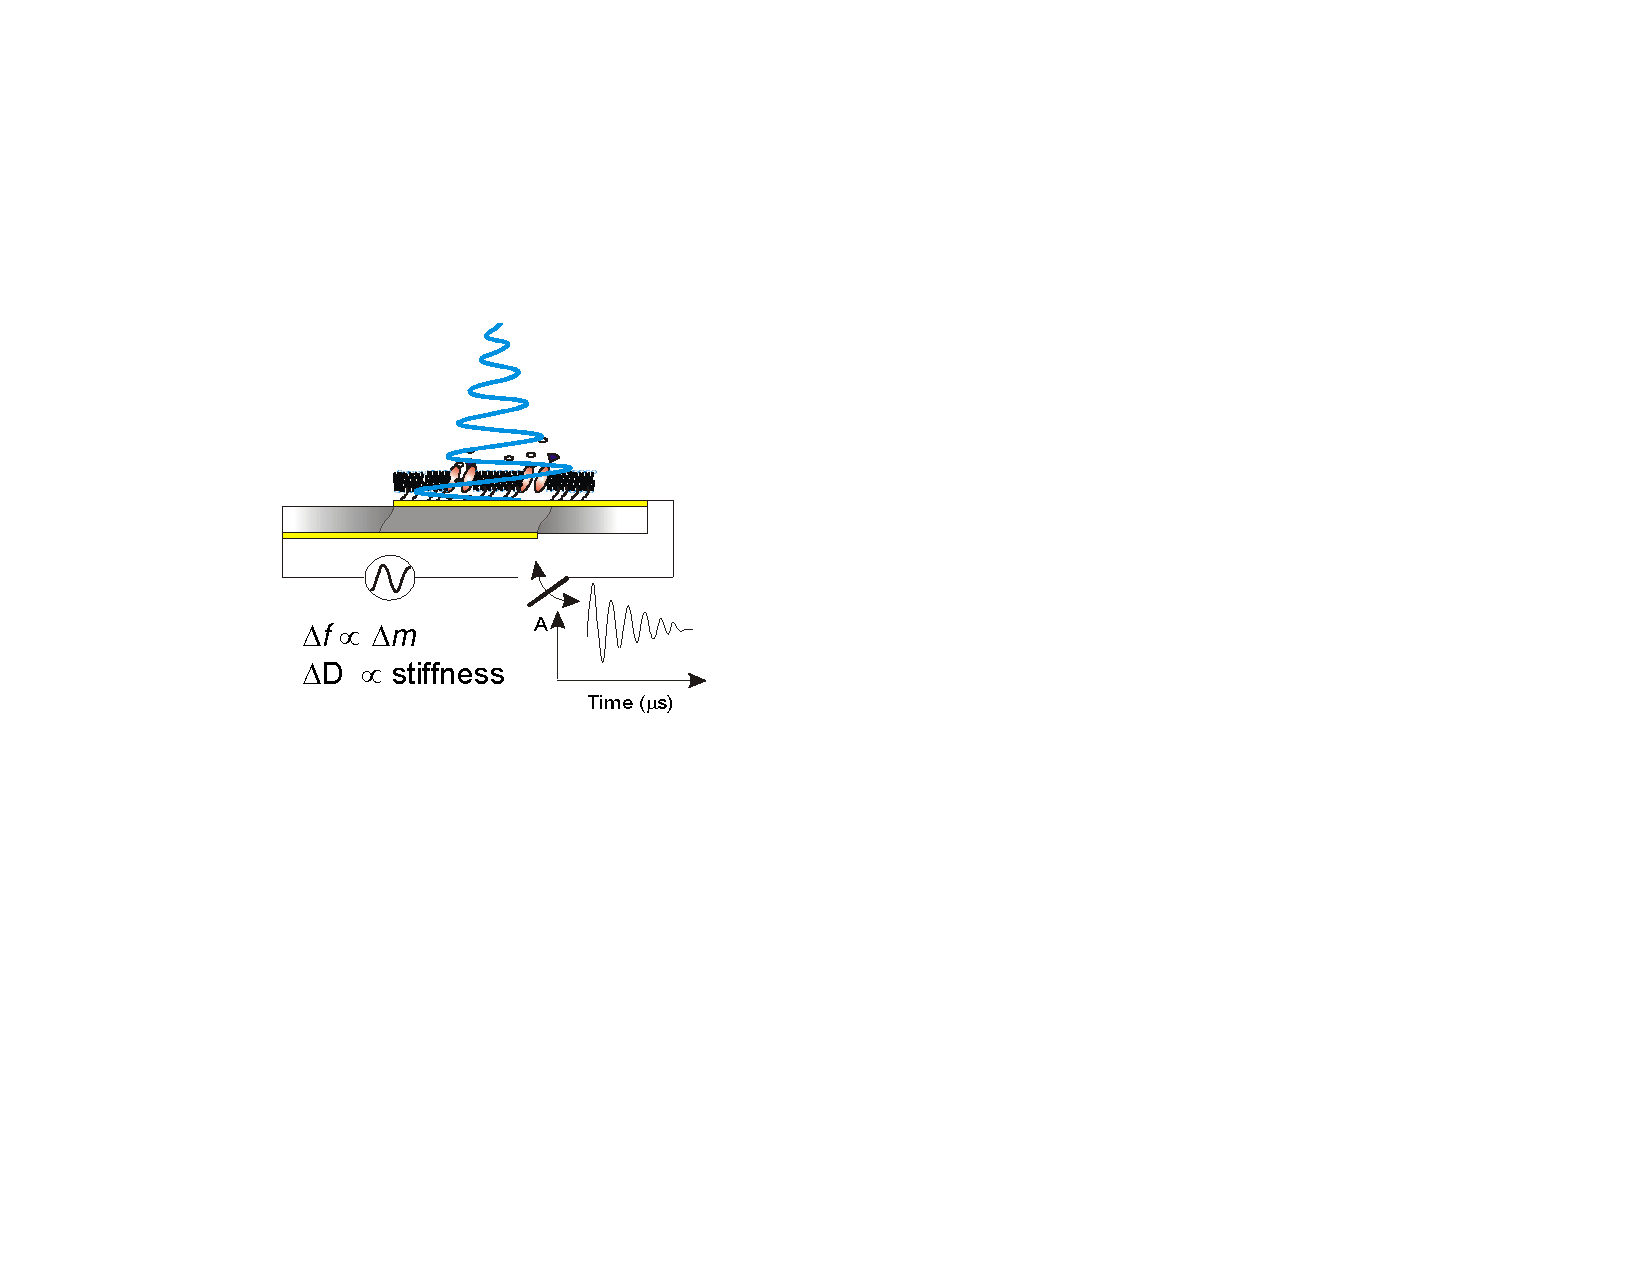
\includegraphics[width=.35\columnwidth]{Mechanical_vs_QCM} &
    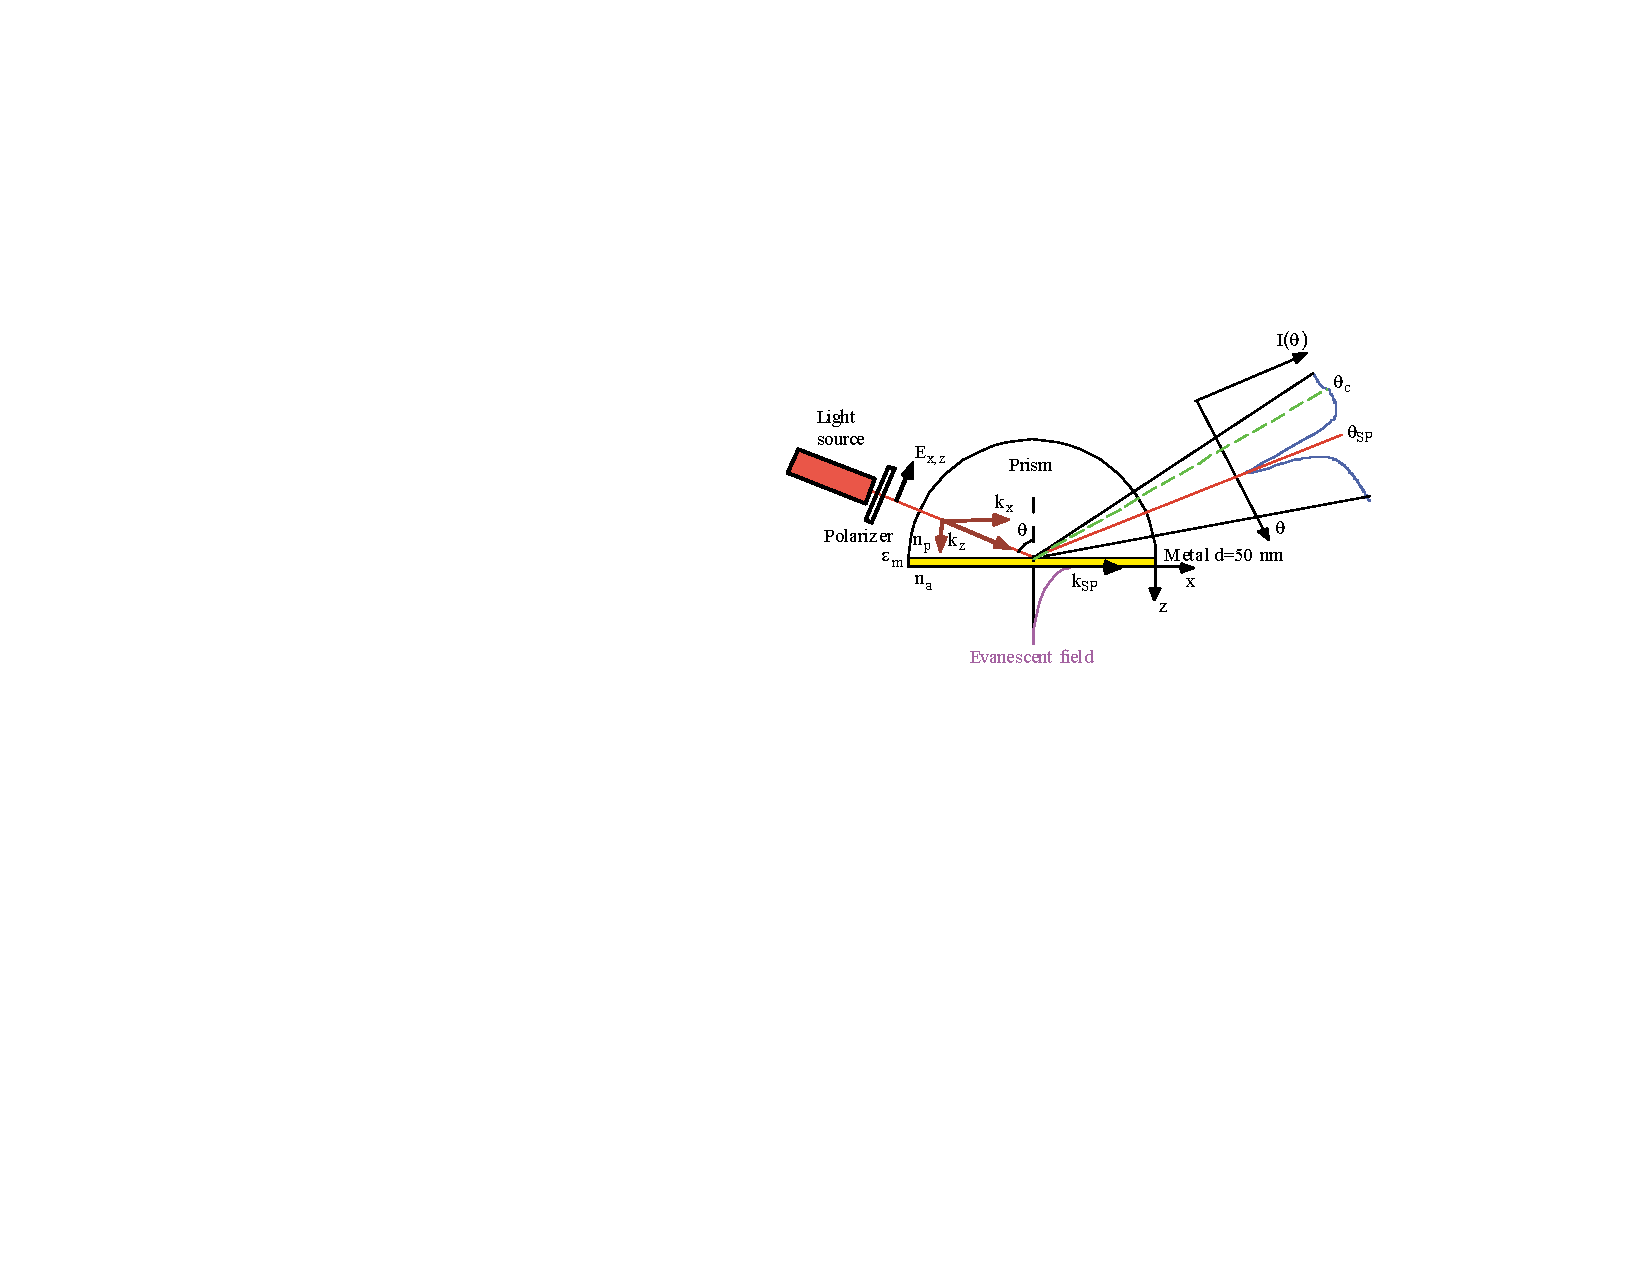
\includegraphics[width=.5\columnwidth]{Mechanical_vs_SPR}
    \\\addlinespace
    \highlight{$\Delta m = -\frac{C}{n} \Delta f_n$} &
    \highlight{$\textstyle \Delta m = d\,\frac{n\ped{protein} - n\ped{buffer}}{\diff n/\diff c}$}
    \\\addlinespace
    $\textrm{LOD}\ped{QCM} = C\cdot \delta f     \simeq \unitfrac[1]{ng}{cm^2}$ &
    $\textrm{LOD}\ped{SPR} = C\cdot \delta\theta \simeq \unitfrac[0.1]{ng}{cm^2}$
\end{tabular}
%%%%%%%%%%%%%%%%%%%%%%%%%%%%%%%%%%%%%%%%%%%%%%%%%%%%%%
\subsection{QCM: Quartz Crystal Microbalance}
%
\formbox{Resonance cond.}{f = \frac{n\,v}{\lambda} = \frac{n\,v}{2t}}
\formula{Dissipation}{D = \frac{1}{\pi f\tau},}
$\tau$: time until $\frac{U\ped{max}}{\eu}$

\vspace{-9mm}
\begin{minipage}{\linewidth}
    \hfill
    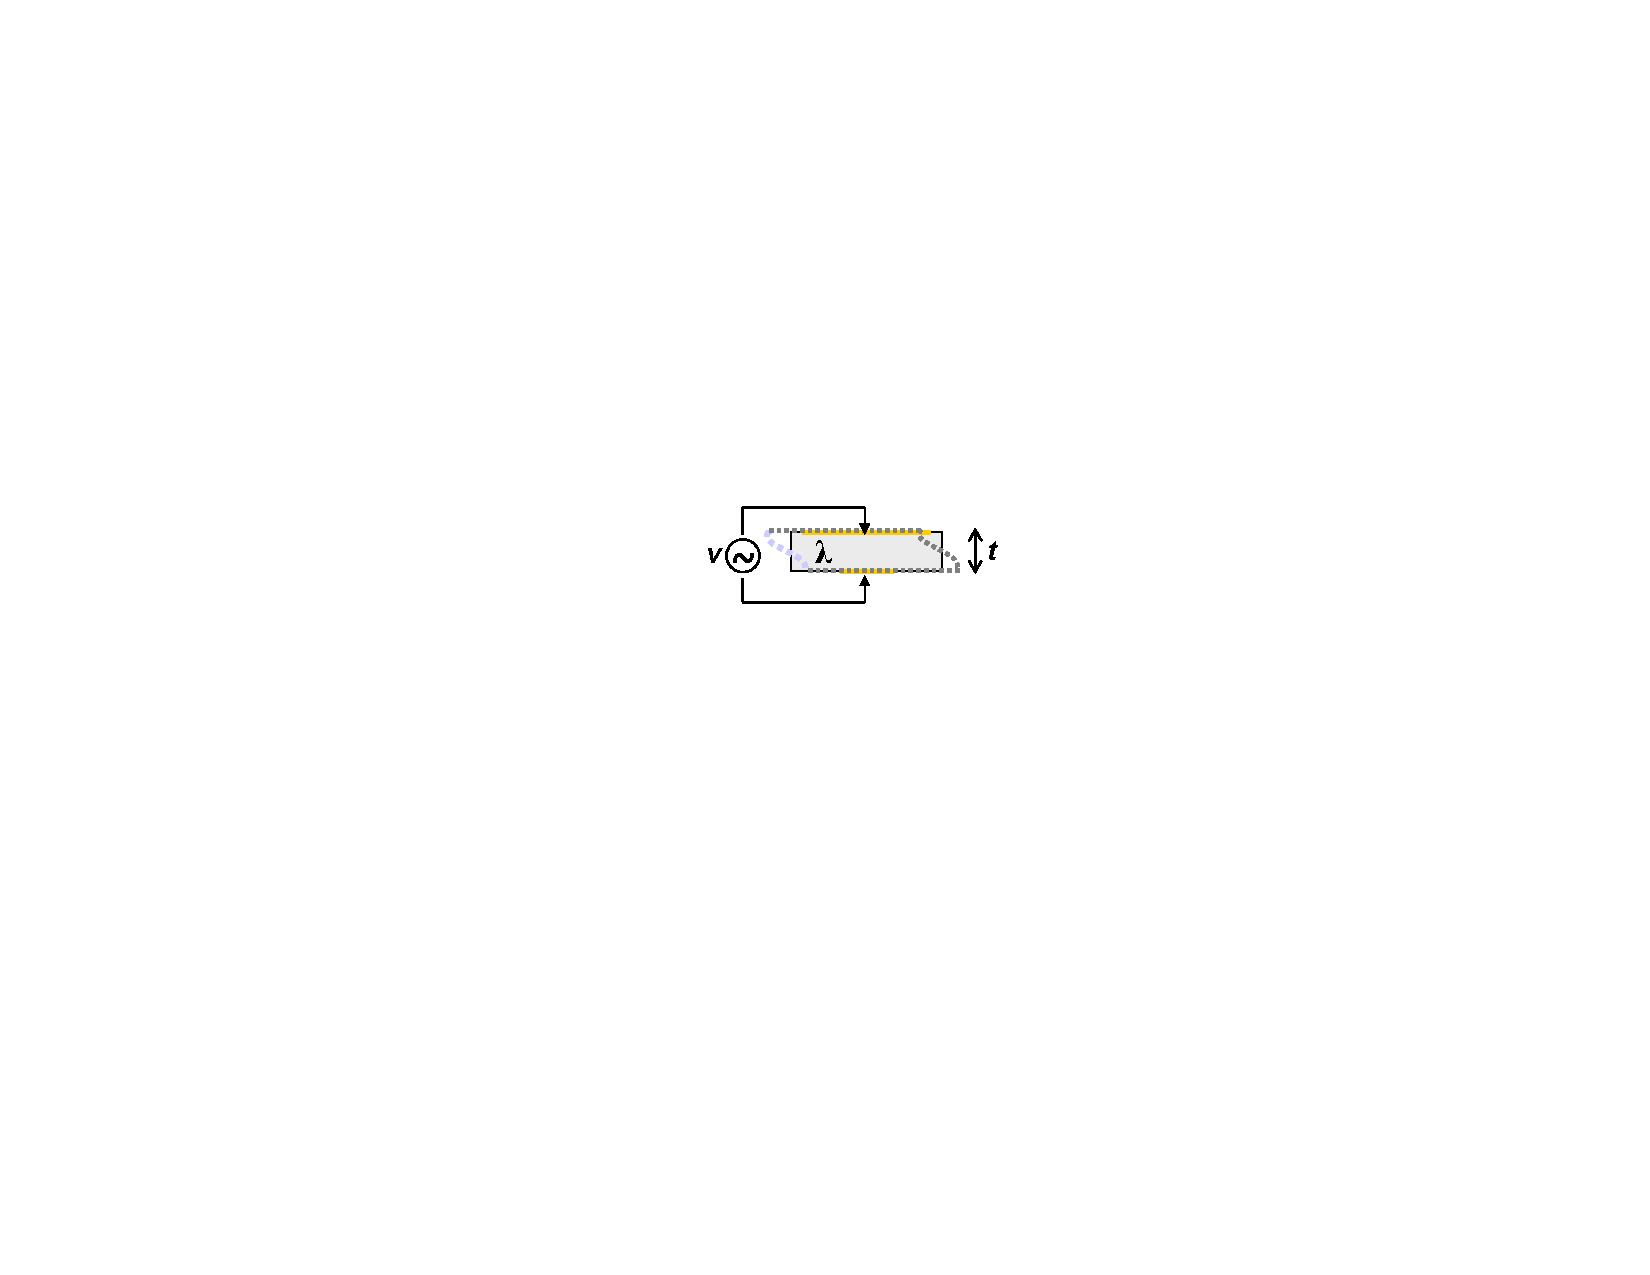
\includegraphics[width=.23\columnwidth]{Mechanical_QCM}
\end{minipage}
\vspace{2mm}

\textbf{Modeling of the QCM-D response} in air / aqueous solution:\par
\begin{minipage}{.25\columnwidth}
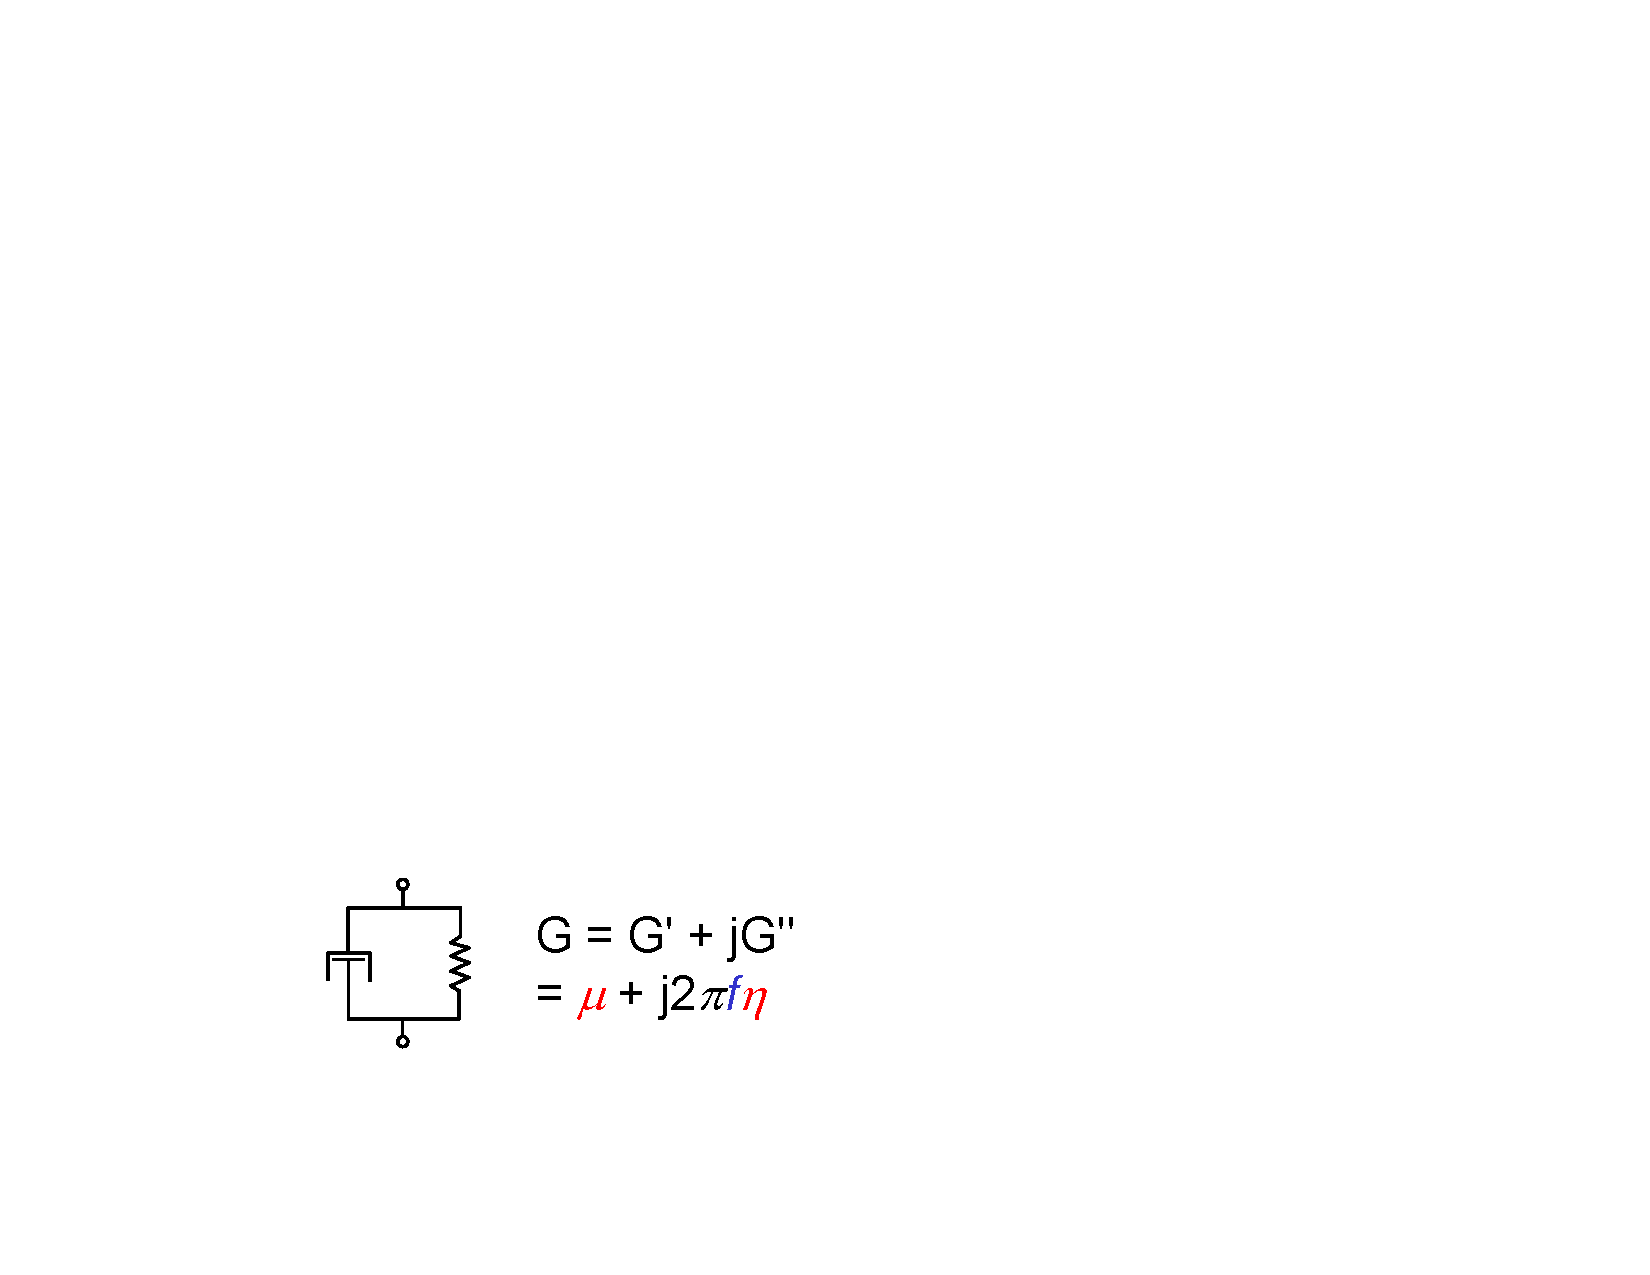
\includegraphics[width=.88\columnwidth]{Mechanical_QCM_Modeling}
\end{minipage}%
\begin{minipage}{.75\columnwidth}
$\eta$: viscosity ($=\frac{G''}{\omega}$), $\mu$: elasticity ($=G'$),\\
$\rho$: density, $d$: thickness
%\formula{Resonance condition}{f = \frac{n\,v}{\lambda} = \frac{n\,v}{2t}}
\end{minipage}
%%%%%%%%%%%%%%%%%%%%%%%%%%%%%%%%%%%%%%%%%%%%%%%%%%%%%%
\subsection{Strain Gauge}
%
\formula{Resistive strain g.}{\frac{\Delta R}{R} = k\,\frac{\Delta l}{l} = k\,\epsilon
\textrm{,\enskip $\epsilon$: Strain, $k$: Gauge factor}}
\formula{Capacitive strain g.}{C = \epsilon_0\epsilon_r\,\frac{A}{d} \textrm{,\enskip (displacement: $d \to d+\Delta d$)}}

		%! Author = tstreule

\section{Fluorescent Probes}
%%%%%%%%%%%%%%%%%%%%%%%%%%%%%%%%%%%%%%%%%%%%%%%%%%%%%%
%%%%%%%%%%%%%%%%%%%%%%%%%%%%%%%%%%%%%%%%%%%%%%%%%%%%%%
\subsection{Fluorescence Statistics}
%
\textbf{Photobleaching}: A fluorescent molecule can emit a limited \#photons by excitation before it irreversibly converts to a non-fluorescent molecule.

\begin{minipage}{.3\columnwidth}
    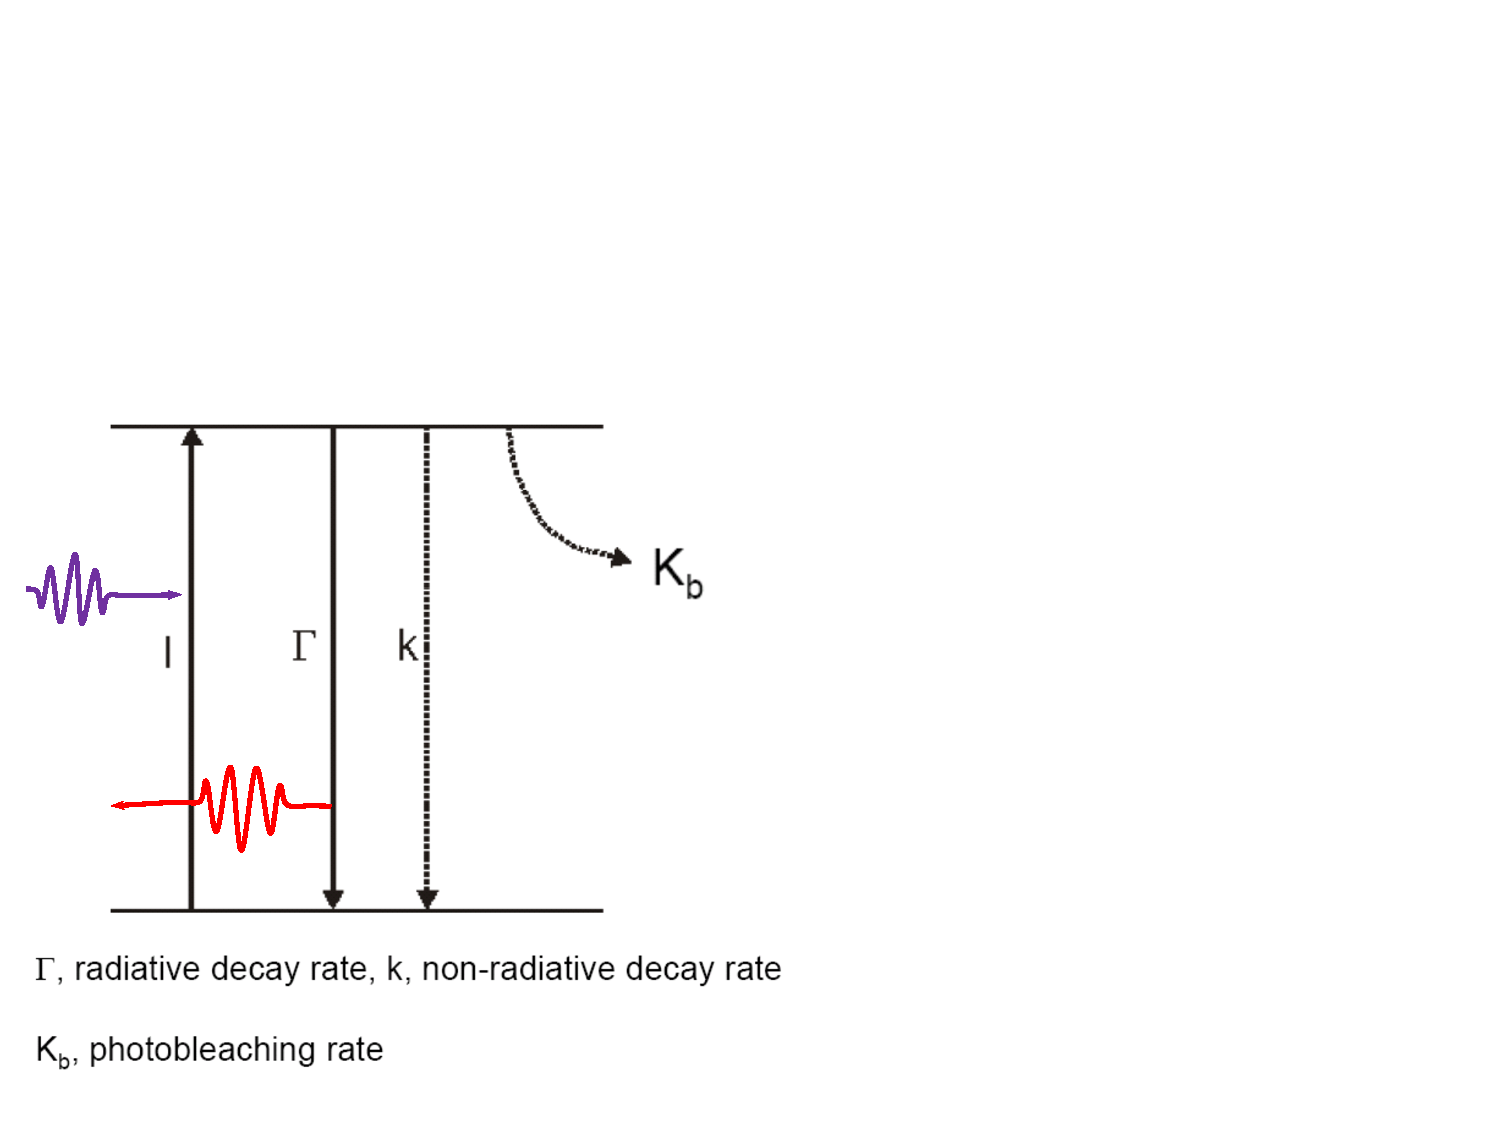
\includegraphics[width=.9\columnwidth]{Fluorescence_Statistics}
\end{minipage}%
\begin{minipage}{.7\columnwidth}
    \formula{\textbf{Quant. Yield}}{Q = \frac{\Gamma}{\Gamma+k+K_b} \sim 0-98\%}
    \hfill (Efficiency)
    \formbox{Fluorescence \textbf{Lifetime}}{\tau = \frac{1}{\Gamma+k+K_b} \sim \unit[1]{ns}}
    \vspace{1mm}

    Fluorescence emission is a statistical process that is characterized by exponential decays.
    \formula{Molecules in \textit{excited} state}{\deriv{N_e}{t} = -\left(\frac{1}{\tau_1}+\ldots+\frac{1}{\tau_n}\right) N_e}
\end{minipage}
%%%%%%%%%%%%%%%%%%%%%%%%%%%%%%%%%%%%%%%%%%%%%%%%%%%%%%
\columnbreak
\subsection{FRET \textnormal{-- Fluorescence Resonance Energy Transfer}}
%
\begin{minipage}{.25\columnwidth}
    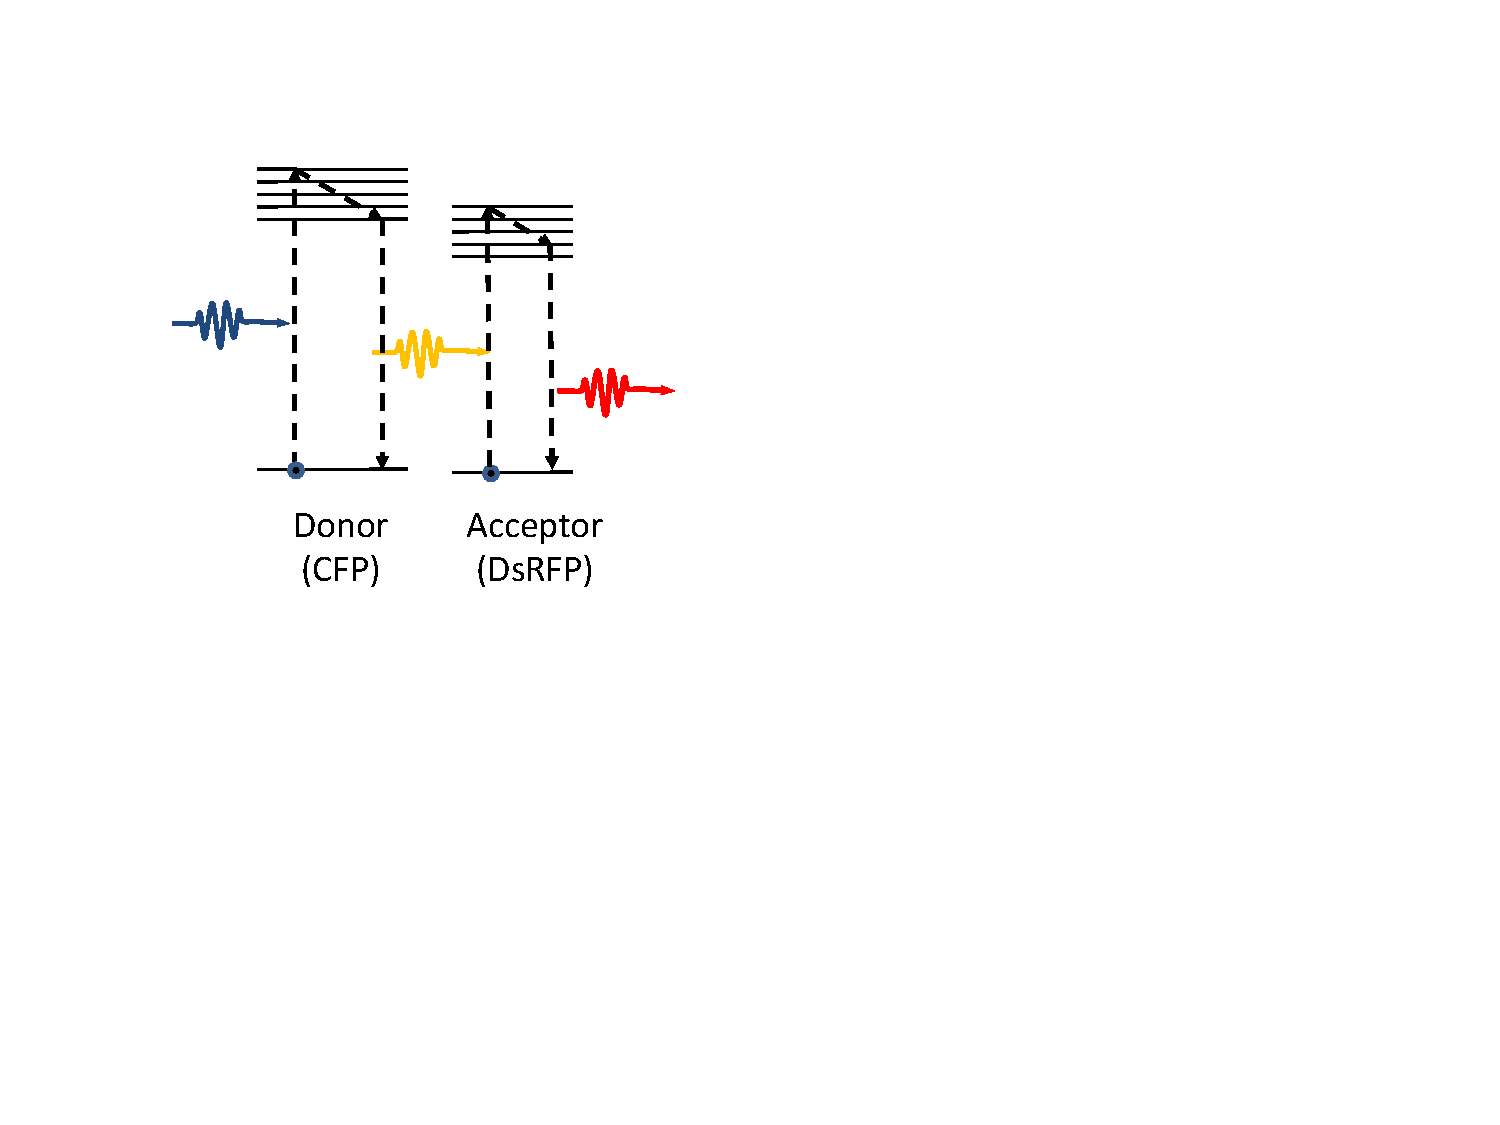
\includegraphics[width=.9\columnwidth]{Fluorescence_FRET}
\end{minipage}%
\begin{minipage}{.75\columnwidth}
    Seeing a different $\lambda\ped{emission}$ tells us that two molecules are close.
    \formbox{Efficiency}{E = \frac{R_0^2}{R_0^2+r^6} = 1\!-\!\frac{\tau\ped{DA}}{\tau\ped{D}} = 1\!-\!\frac{I\ped{DA}}{I\ped{D}}}
    where
    \formtex{$\tau\ped{D(A)}$, $I\ped{D(A)}$}{Lifetime/Intensity of donor emission}
    
    \formtex{~}{in the absence/presence of acceptor.}
\end{minipage}
%%%%%%%%%%%%%%%%%%%%%%%%%%%%%%%%%%%%%%%%%%%%%%%%%%%%%%
\subsection{Calcium Imaging \textnormal{\hfill $\to$ too slow for $t$ dependency meas.}}
%
Calcium ion cannot be visualized/tagged directly:
$\to$
Design molecules with optical properties that change upon calcium binding.

\begin{minipage}{.23\columnwidth}
    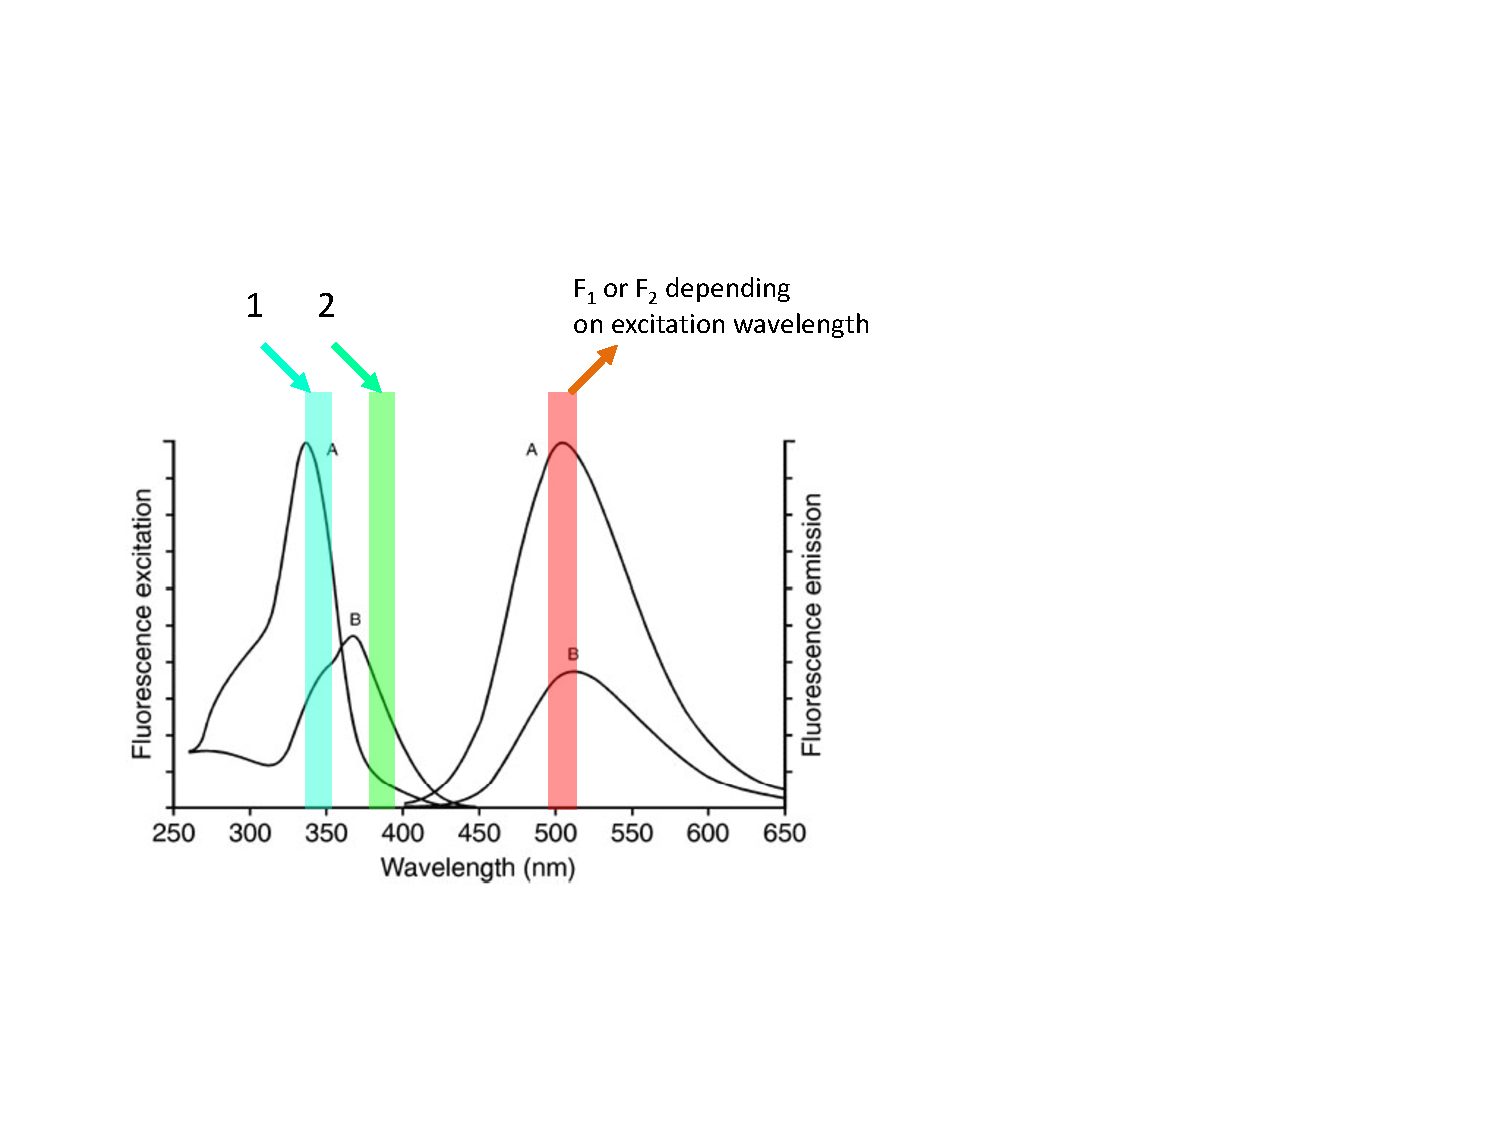
\includegraphics[width=\columnwidth]{Fluorescence_Calcium_Imaging}
\end{minipage}%
\hspace{\columnsep}%
\begin{minipage}{.77\columnwidth-\columnsep}
    \textbf{Single \& dual wavelength measurements}: 
    \formbox{Concentration}{[\ce{Ca^{2+}}]_i = K\ped{d,eff} \frac{R-R\ped{min}}{R\ped{max}-R}}
    where
    \formula{for single}{\scriptstyle R\equiv F \text{ and } K\ped{d,eff} = \frac{[\ce{Ca^{2+}}]_i \times(F\ped{max}-F)}{F-F\ped{min}}}
    \formula{for dual.}{R=F_1/F_2}
    \qquad ($F$: fluorescence)
%
%		where $R=F_1/F_2$ for dual wavelength and $R\equiv F$ and $K\ped{d,eff} = \frac{[\ce{Ca^{2+}}]_i \times(F\ped{max}-F)}{F-F\ped{min}}$ for single wavelength
\end{minipage}

The binding of \ce{Ca^{2+}} leads to\ldots
\begin{itemize}
    \item change in fluorescence \textbf{intensity} but not wavelength change
    \item a \textbf{shift} in excitation (and/or emission) peaks (``dual wavelength'')
    \item changes in fluor. resonance energy transfer (\textbf{FRET}) \& life time
\end{itemize}
%%%%%%%%%%%%%%%%%%%%%%%%%%%%%%%%%%%%%%%%%%%%%%%%%%%%%%
\subsubsection{Delivery of Calcium Indicators}
%
\formtex{\textbf{Loading cells}}{Once the molecule got cleaved (spalten), it}
\formtex{~}{cannot go out and gets fluorescent.}

\formtex{Introduce \textbf{fluoresc.}}{Proteins change emission rate when \ce{Ca} binds.}
\formtex{\textbf{proteins} or (natural)}{Relative change ($\Delta F/F$) in fluorescence}
\formtex{\textbf{FRET proteins}}{emission of EGFP can then be meas. directly.}

\underline{Note}: The dye responds \textit{fast}, but it is \textit{slow} to recover. \ce{Ca} dissociation\\
\phantom{\underline{Note}:} rate (i.e. recovery) depends on dye’s affinity for \ce{Ca}.

		%! Author = tstreule

\section{Detection and Noise}
%%%%%%%%%%%%%%%%%%%%%%%%%%%%%%%%%%%%%%%%%%%%%%%%%%%%%%
%%%%%%%%%%%%%%%%%%%%%%%%%%%%%%%%%%%%%%%%%%%%%%%%%%%%%%
\subsection{Signal}
%
For statistically independent, ``uncorrelated'', events we use\\
\begin{minipage}{.3\columnwidth}
    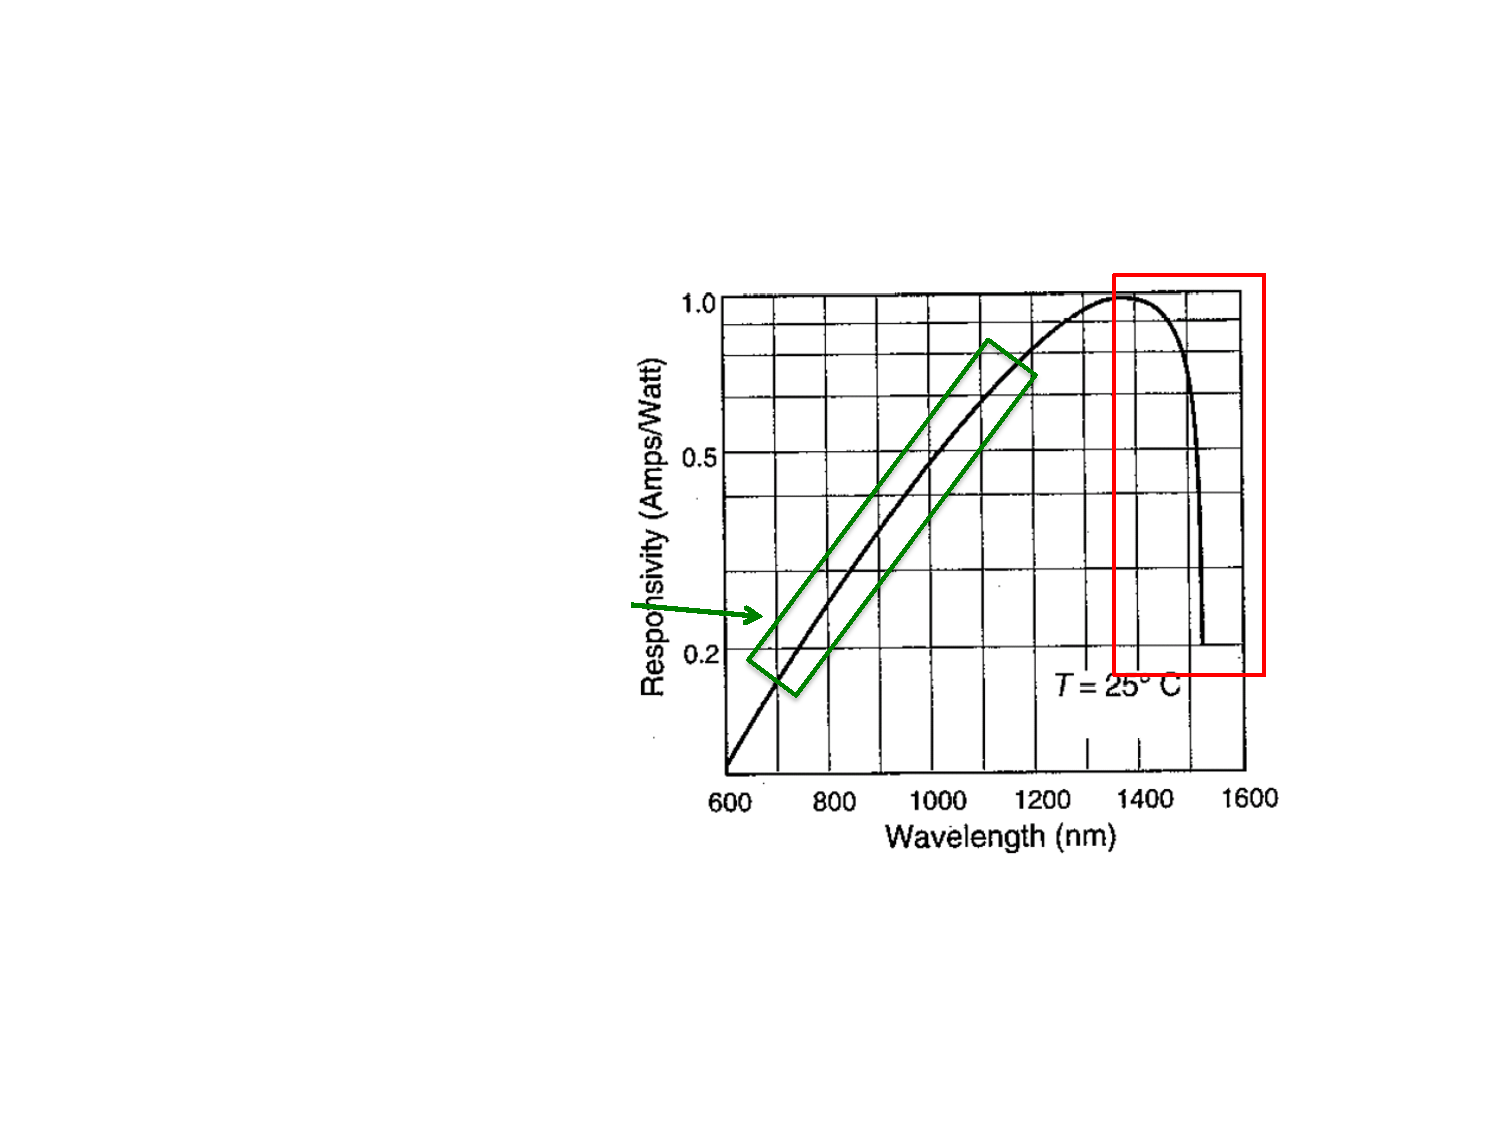
\includegraphics[width=.9\columnwidth]{Noise_QE_and_Responsivity}
\end{minipage}%
\begin{minipage}{.7\columnwidth}
    \formbox{\textbf{Poisson}}{P_{\overline{n}}(n)= \frac{\overline{n}^n}{n!} \eu^{-\overline{n}}}
    \parbox{.25\columnwidth}{$\overline{n}$: mean\\$\sigma_n \!=\! \sqrt{\overline{n}}$: var}
    \formula{Signal current}{\avg{I\ped{sig}} = \eta q\overline{n}/\Delta t}
    \formula{\textcolor[rgb]{0.23,0.49,0.14}{Responsivity}}{\avg{I\ped{sig}}/P = \eta q\lambda/(hc)}
    \formula{\textcolor{red}{Cutoff $\lambda$}}{\lambda(\unit{\mu m}) = 1.24/E(\unit{eV})}
\end{minipage}
%%%%%%%%%%%%%%%%%%%%%%%%%%%%%%%%%%%%%%%%%%%%%%%%%%%%%%
\subsubsection{Fundamental Noise Sources}
%
\formula{Noise\hfill \textbf{shot}}{N\ped{s} = 2R\eta qB \avg{I\ped{sig}} = \avg{I\ped{shot}^2} R \;,}
$2B \simeq 1/\Delta t$
\formula{\hfill \textbf{dark}}{N\ped{d} = 2R\eta qB \avg{I\ped{dark}}}
\vspace{-2mm}
\formula{\hfill thermal}{N\ped{J} = \avg{I\ped{Johnson}^2} R = \sqrt{\frac{k\ped{B}TB}{R}}^2 R}
\formula{\hfill \textbf{readout}}{N\ped{r} = N\ped{J}+N\ped{amplifier}}
\formbox{~}{N\ped{tot} = N\ped{s}+N\ped{d}+N\ped{r}}
$\sigma\ped{tot}^2 = \sum \sigma_i^2$
\formbox{SNR}{\textrm{SNR}\ped{curr} = \frac{\eta\cdot N_\gamma}{\sqrt{ \eta N_\gamma + N_d + N_r }}}
$\eta = \textrm{QE} \cdot absorb$
\formula{\centering for large numbers}{\textrm{SNR}\ped{shot} = \frac{\overline{n}}{\sqrt{\overline{n}}} = \sqrt{\overline{n}} \;\;\widehat{=}\;\; \eta N_\gamma}
%%%%%%%%%%%%%%%%%%%%%%%%%%%%%%%%%%%%%%%%%%%%%%%%%%%%%%
\subsection{(Optical) Detectors}
%
%	Characterizing Photodetectors
%	\begin{enumerate}
%		\item Quantum Eff.:
%			probability of generating a photoelectron
%		\item Internal Amplification:
%			ratio for converting a photoelectron into an output current
%		\item Dynamic Range:
%			largest and lowest (linearly) measurable signal
%		\item Response Speed:
%			$\Delta t$ and spread between incoming photon and output current burst
%		\item Geom. form factor:
%			Size and shape of the active area and the detector
%		\item Noise:
%			Shot noise vs. read-out noise dominated
%	\end{enumerate}
%
\formbox{\textbf{Photoel. effect}}{E\ped{ph} = hf = hc/\lambda = \phi + E\ped{kin}}
\formtex{~}{incident $E\ped{ph}$ = $E\ped{binding}$+$E\ped{kin}$ of ejected el.}
\formbox{Photo mult. (PMT)}{I = \alpha\;(S\cdot E\ped{ph}\,n/\Delta t) \;,}
$S$: sensitivity, $N\ped{d}\uparrow$

Choose \textbf{binning mode} (2x2, 4x4, …) such that the pixel size of the camera fits the best the maximum pixel size.
\formbox{\textbf{max. pixel size}}{\textrm{max} = 0.3 \frac{\lambda}{\textrm{NA}} \times M}\\
%%%%%%%%%%%%%%%%%%%%%%%%%%%%%%%%%%%%%%%%%%%%%%%%%%%%%%
%	\begin{center}
%		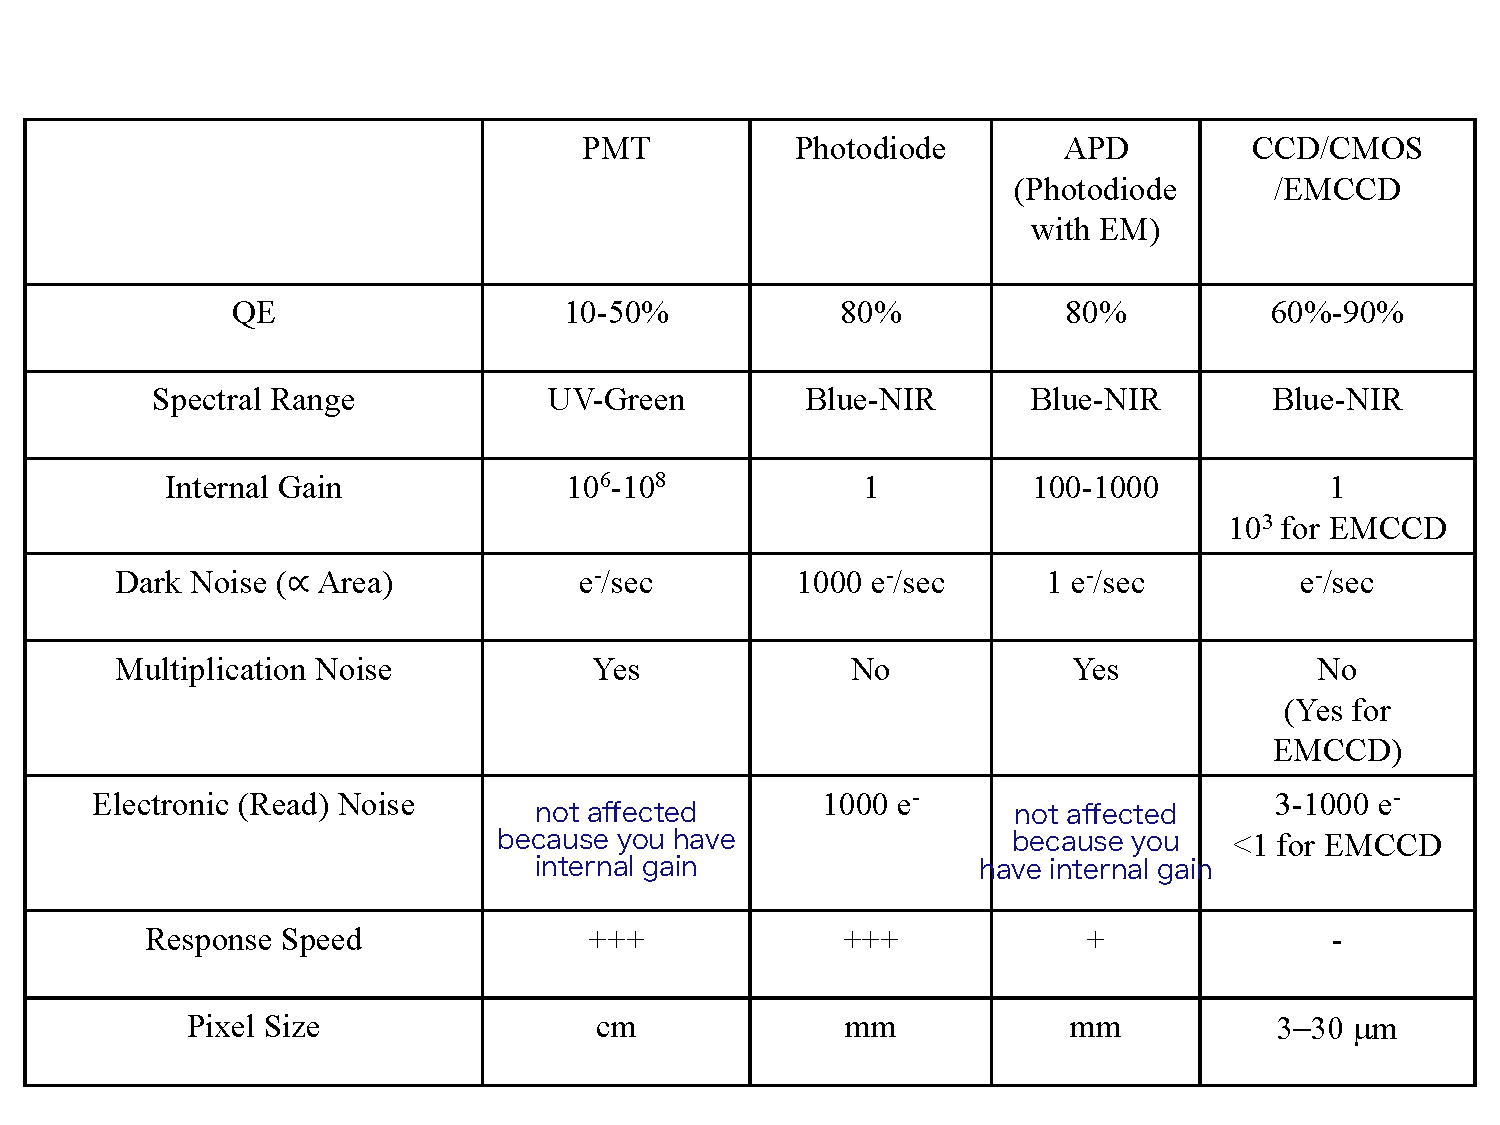
\includegraphics[width=.8\columnwidth]{Detection_Comparison}
%	\end{center}
%%%%%%%%%%%%%%%%%%%%%%%%%%%%%%%%%%%%%%%%%%%%%%%%%%%%%%
\subsection{Imaging Deep Tissues}
%
%	\textbf{Thick sample}: light will scatter, illuminating parts don't want to: SNR$\downarrow$
\formbox{Beer-Lambert's law}{I = I_0\,\eu^{-\mu\,x}}

\begin{minipage}{.5\columnwidth}
    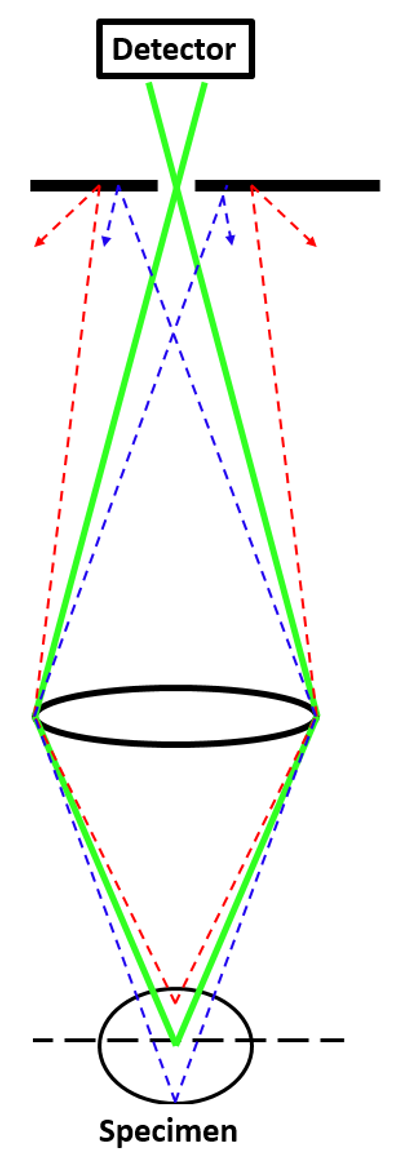
\includegraphics[width=.2\columnwidth]{Detection_Confocal_2}%
    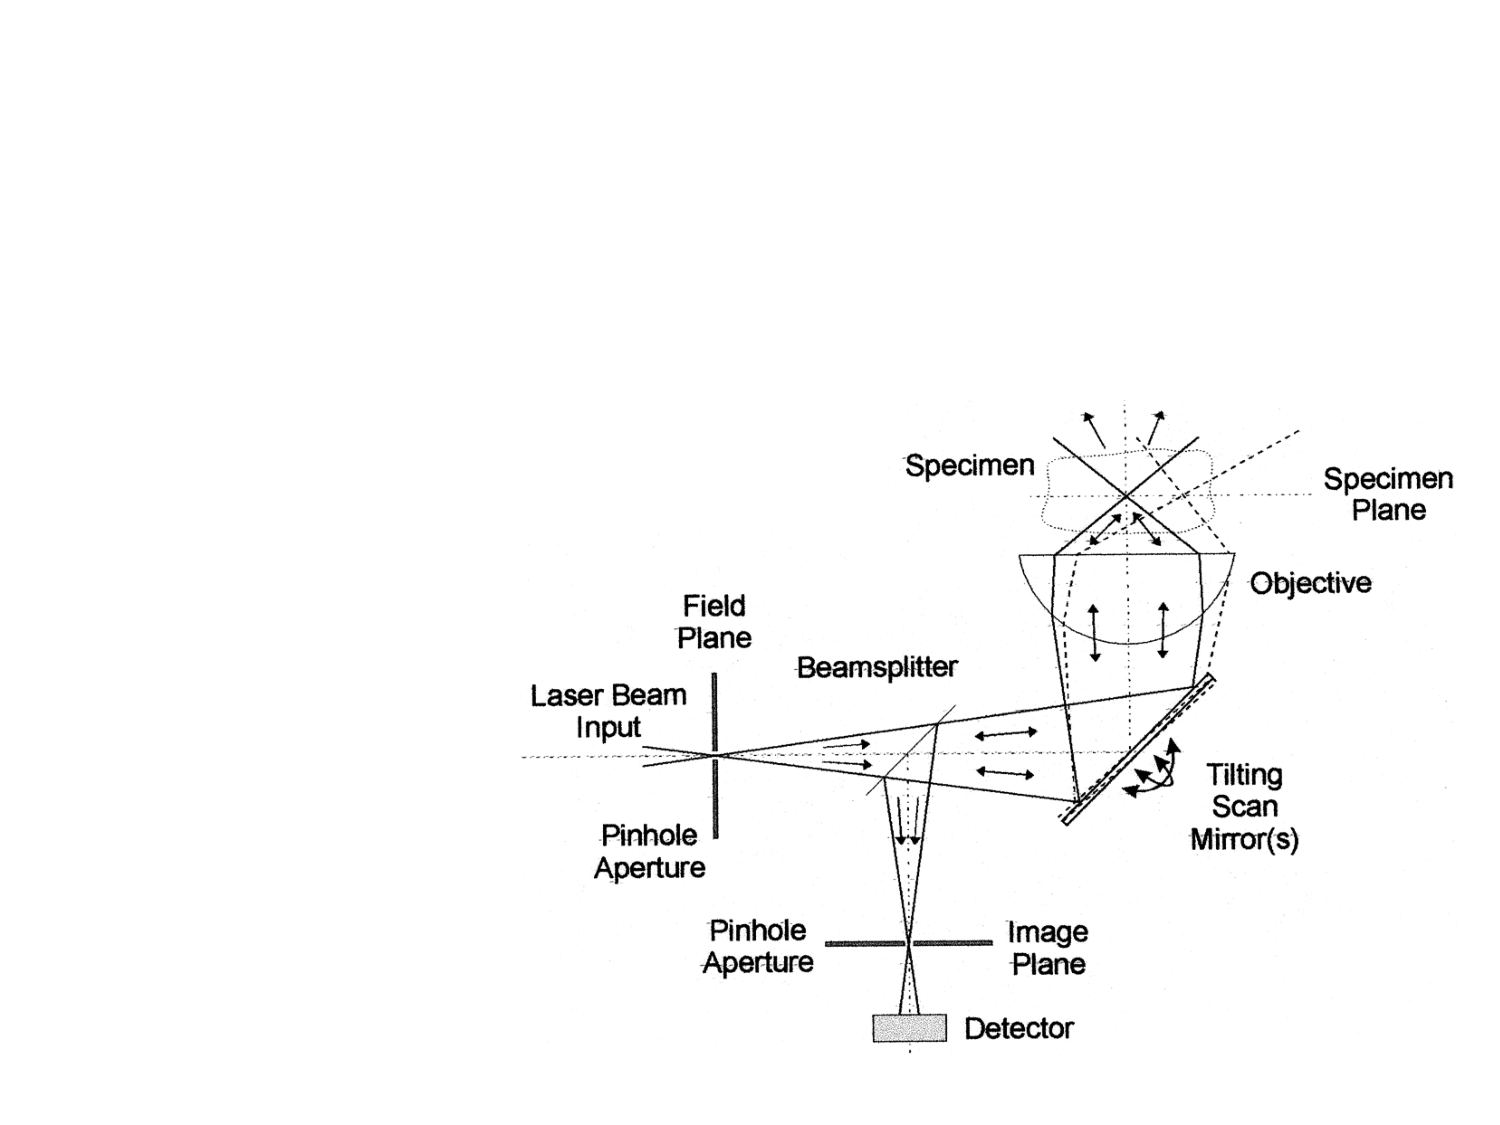
\includegraphics[width=.75\columnwidth]{Detection_Confocal_1}
\end{minipage}%
\begin{minipage}{.5\columnwidth}
    \textbf{1st} Pinhole by illumination:\\
    $\to$ focus the illum. to a small spot

    \textbf{2nd} Pinhole by detector:\\
    $\to$ reject out of focus light\\
    $\to$ collect light to PMT

    Signal and Noise (\textbf{Pinhole size}):\\
    $\bullet$ more out of focus light $\to$ blurry\\
    $\bullet$ less in-focus light $\to$ SNR$\downarrow$
\end{minipage}

\formbox{Choose \textbf{pinhole size}}{\sim\!\!\Delta r = 0.61 \frac{\lambda}{\textrm{NA}} \times M}
%%%%%%%%%%%%%%%%%%%%%%%%%%%%%%%%%%%%%%%%%%%%%%%%%%%%%%
\subsubsection{2ph-Excitation}
%
\begin{minipage}{.3\columnwidth}
    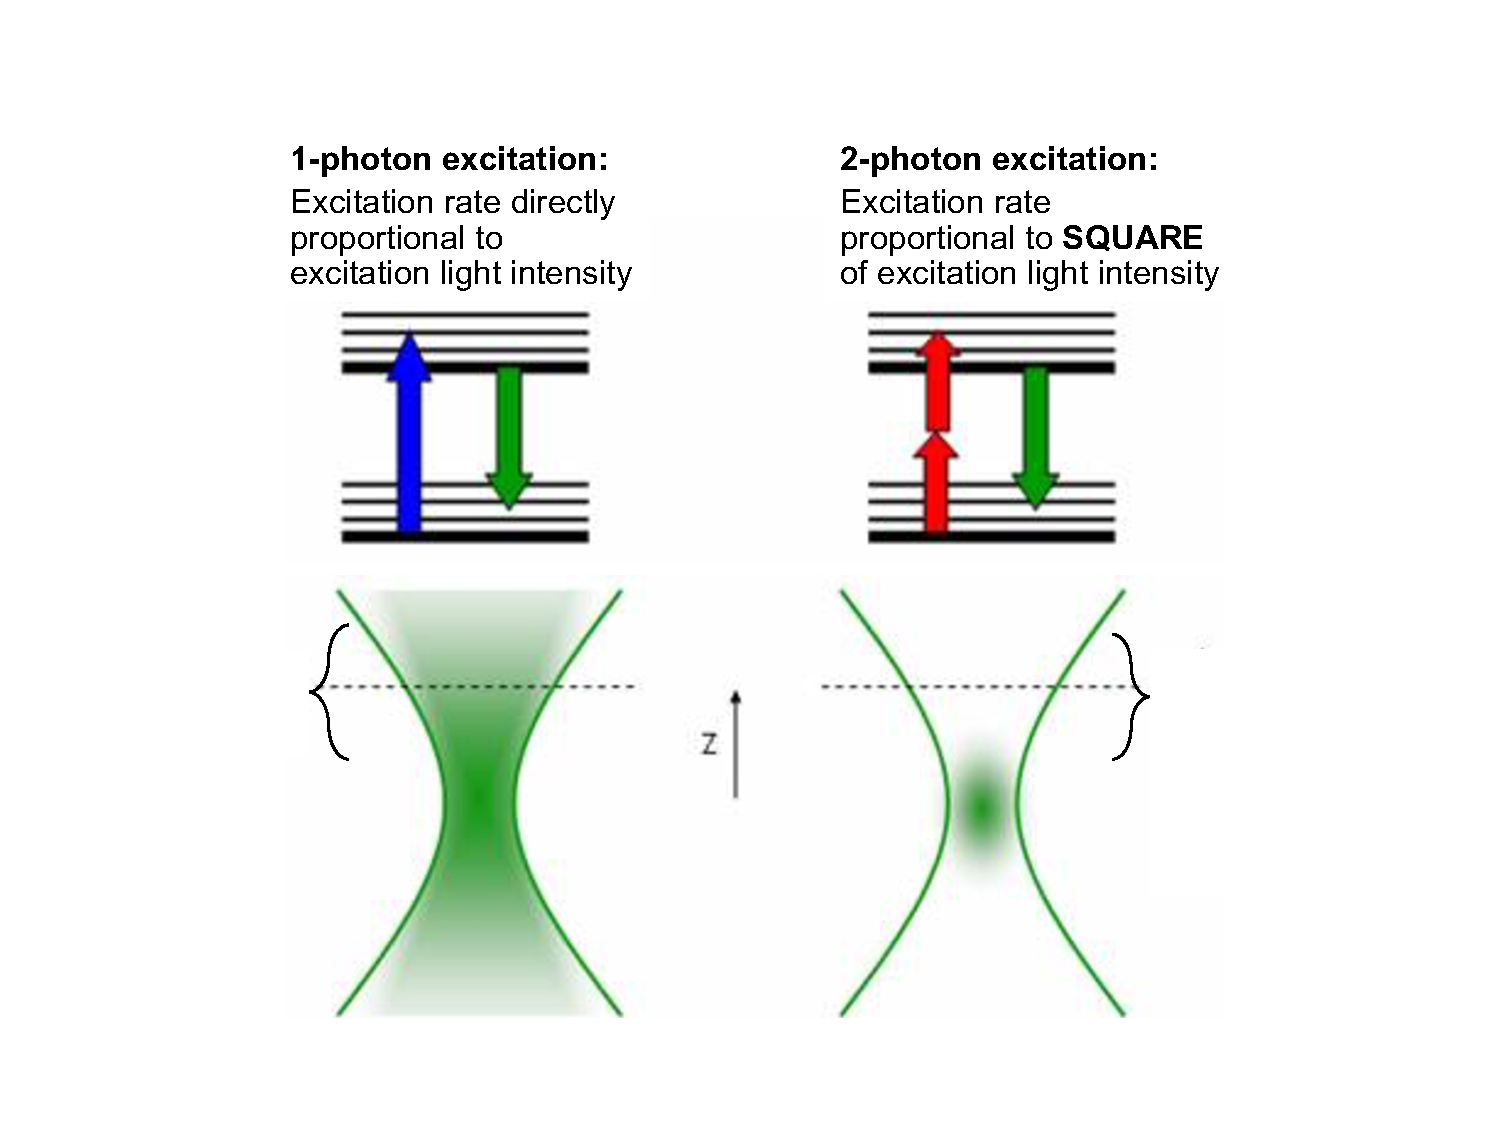
\includegraphics[width=.9\columnwidth]{Detection_2ph_Excitation}
\end{minipage}%
\begin{minipage}{.7\columnwidth}
    \begin{itemize}
        \item[+] wavelength$\uparrow$ $\to$ less absorbing/scattering
        \item[+] photons need to coincide in space and time to excite
        \item[+] No pinhole by detector for 2ph: Collect all the light
        \item[--] low prob. of occurrence i.e. inefficient
        \item[--] ultra-short pulse light source needed
    \end{itemize}
\end{minipage}

		%! Author = tstreule

\section{Optical Biosensors}
%%%%%%%%%%%%%%%%%%%%%%%%%%%%%%%%%%%%%%%%%%%%%%%%%%%%%%
%%%%%%%%%%%%%%%%%%%%%%%%%%%%%%%%%%%%%%%%%%%%%%%%%%%%%%
%	\subsection{Optical Methods}
%	%
%	\begin{itemize}
%		\item \underline{Reflection based} (ELM, SAR)\\
%			information through $\Delta\phi$ and $\Delta$amplitude
%		\item \underline{Interference based} (OIA, TINS)\\
%			information through color change \quad
%			very sensitive to $\Delta$thickness
%		\item \underline{Evanescent field} techniques (\textbf{SPR}, \textbf{OWLS}, RM, FTIR, SAR)\\
%			information through $\Delta n$ ($n$: refractive index)
%	\end{itemize}
%%%%%%%%%%%%%%%%%%%%%%%%%%%%%%%%%%%%%%%%%%%%%%%%%%%%%%
\subsection{EM}
%
\textbf{Relations}:\\
$c_0 = \frac{1}{\sqrt{\epsilon_0\mu_0}}$ \hfill
$k_0 = \frac{2\pi}{\lambda_0} = \frac{\omega}{c_0} = \omega\sqrt{\epsilon_0\mu_0}$ \hfill
$k = \frac{2\pi n}{\lambda}$ \hfill
$n = \frac{c_0}{c} = \sqrt{\epsilon_r\mu_r} \simeq \sqrt{\epsilon_r}$
\formula{Dispersion relation}{k^2 = \epsilon\omega^2 = \epsilon k_0^2c_0^2 = k_0\frac{\epsilon}{\epsilon_0} = k_0^2\epsilon_r = (k_0n)^2}

\formbox{\textbf{Plane waves}}{\vec{E}(\vec{r},t) = \vec{E}_0\;\eu^{\iu(\vec{k}\vec{r}-\omega t)}} \\
whereby \hfill
$\partial_t \hat= -\iu\omega$, \hfill
$\partial_x \hat= \iu k_x$, \hfill
$\partial_z \hat= \iu k_z$, \hfill
$\partial_y \hat= 0$ (infinite extent)
\formula{Depth of penetration}{d_p = \frac{\lambda}{4\pi} \frac{1}{\sqrt{n\ped{inc}^2\sin^2\theta -n_2^2}}}
\quad (about $\unit[500]{nm}$)
%%%%%%%%%%%%%%%%%%%%%%%%%%%%%%%%%%%%%%%%%%%%%%%%%%%%%%
\subsection{Evanescent Field Techniques}
%
\formtex{\textit{Recap}}{Always \textbf{total reflection} for $n\ped{inc}>n_2$}
\formtex{Evanescence}{Negligible change of sensitivity compared to}
\formtex{~}{the size of the antibodies}
%%%%%%%%%%%%%%%%%%%%%%%%%%%%%%%%%%%%%%%%%%%%%%%%%%%%%%
\subsubsection{SPR \textnormal{-- Surface Plasmon Resonance}}
%
\formtex{\textbf{Plasmon}}{\underline{quantum} of electron density wave in a metal}
\formtex{\textbf{Plasmon Polariton}}{mixt. of photon (diel.) and el. dens. wave (met.)}
\formtex{\textbf{SPP}}{field components point in dir. of propagation}

\formbox{Dispersion relation}{k_{z,i}^2 = k_0^2\epsilon_i-\beta^2}
\quad $i=d,m$
\formula{Mom. of inc. wave}{\highlight{\beta \coloneqq k_x} = \frac{\omega}{c} \frac{\epsilon_m\epsilon_d}{\epsilon_m+\epsilon_d} = k_0 \cdot N}
\formtex{~}{where $N$ effective refr. index of SP}  % $N = \sqrt{\frac{1}{n_c^2} {+} \frac{1}{\epsilon_m}}$

\begin{minipage}{.3\columnwidth}
    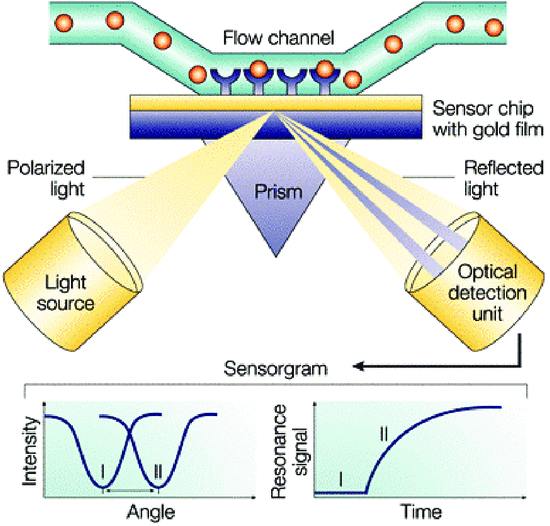
\includegraphics[width=.9\columnwidth]{Optical_SPR}
\end{minipage}\vspace{\boxmargin}
\begin{minipage}{.7\columnwidth-\boxmargin}
    \textbf{Launch a SPP}:
    \quad $0\leq k_{\vert\vert,\textrm{inc}} \leq k_0\;n\ped{inc}$\\
    must ensure \highlight{$\beta \overset{!}{=} k_{\vert\vert,\textrm{inc}} = k_0\;n\ped{inc}\;\sin\theta$}
    \quad $\theta\in[0,\frac{\pi}{2}]$

    $\implies$ \fbox{$n\ped{inc} \geq n\sqrt{\frac{\epsilon_m}{\epsilon_m+n_c^2}}$} \fbox{$\frac{\Delta\theta}{\Delta N} \hat= \pderiv{\theta}{N} = \frac{1}{n\ped{inc}\cos\theta} \simeq \frac{1}{n\ped{inc}}$}
\end{minipage}
%%%%%%%%%%%%%%%%%%%%%%%%%%%%%%%%%%%%%%%%%%%%%%%%%%%%%%
\subsubsection{OWLS \textnormal{-- Optical Waveguide Lightmode Spectroscopy}}
%
\begin{minipage}{.5\columnwidth}
    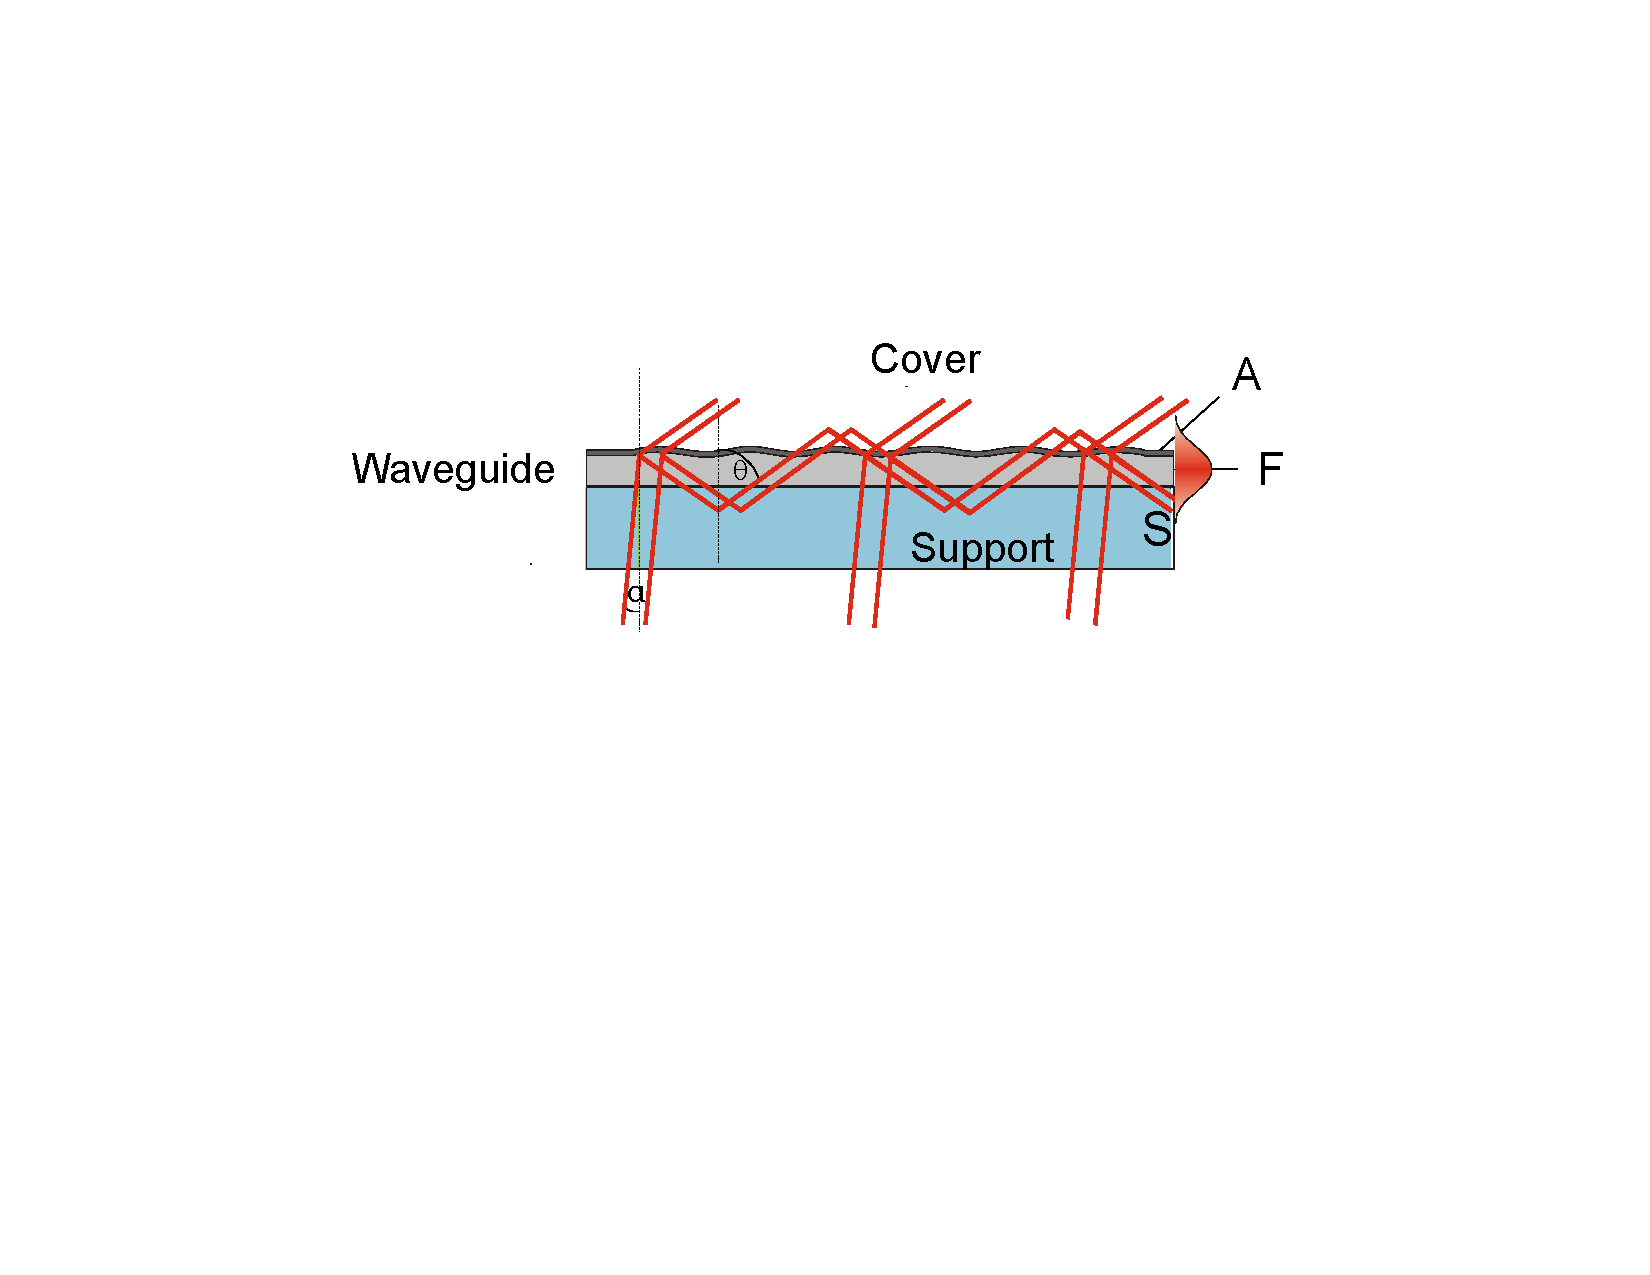
\includegraphics[width=.9\columnwidth]{Optical_OWLS}
\end{minipage}%
\begin{minipage}{.5\columnwidth}
    $N \coloneqq n_F\sin\theta = n\ped{air}\sin\alpha + \frac{l\lambda}{\Lambda}$
    \vspace{2mm}\par
    Penetr. depth \quad \fbox{$\sigma \sim \frac{\lambda}{2\pi} \frac{1}{\sqrt{N^2-n_c^2}}$}
\end{minipage}

Waves have to be in phase (constr. interf.) $\to$ extremely sensitive

\formula{constr. interference}{\textcolor{gray}{0=}\;2\pi m \overset{!}{=} \phi_F + \phi_{FS} + \phi_{FAC}}
\quad $\phi$: phase shifts

\formula{Ansatz for \textit{3 layer model}}{\scriptsize
    \begin{cases}
        \text{Cover:}		& C \;\eu^{-\abs{k_{z,C}} \;(z-d_F/2)}\\
        \text{Waveguide:}	& B \;\eu^{\iu k_{z,F} z} + A \;\eu^{\iu k_{z,F} z}\\
        \text{Support:}	& D \;\eu^{\abs{k_{z,S}} \;(z+d_F/2)}
    \end{cases}
}

\formula{Idealized adlayer}{n_A = n_C + c_A\deriv{n}{c}}
\formbox{Mass calculation}{M = \diff_A \frac{n_A-n_C}{\diff n/\diff c}}
%%%%%%%%%%%%%%%%%%%%%%%%%%%%%%%%%%%%%%%%%%%%%%%%%%%%%%
\subsection{Limitations}
%
%	Above methods are \textit{not usable for diagnostic purposes}.\\
%	For analyzing \textit{simple things} it is extremely accurate, but when the composition of the probe gets more complex (e.g. blood) your device is not usable.\\
%	However, because of the NSB problems, we cannot use it (see LOD).
Above methods not usable for \textit{diagnostic purpose} $\to$ NSB, LOD

\textbf{Solution}: diffractometric biosensors (Focal Molography)

		%! Author = tstreule

\section{Molecular Adsorption and Electron Transfer}
%%%%%%%%%%%%%%%%%%%%%%%%%%%%%%%%%%%%%%%%%%%%%%%%%%%%%%
%%%%%%%%%%%%%%%%%%%%%%%%%%%%%%%%%%%%%%%%%%%%%%%%%%%%%%
\subsection{Quantum Mechanics}
%
\formula{Schrödinger eq.}{\hat{H}\psi(\vec{r}) = E\psi(\vec{r})}
\quad where $\hat{H} = -\frac{\hbar}{2m}\pderiv[2]{~}{x} + V$

\formula{\textbf{1D potential well}}{\psi(x) = \sqrt{\frac{2}{L}} \sin(k_nx)}
\quad for $0\leq x\leq L$
\formtex{~}{where $k_n = \frac{n\pi}{L}$, $n\in\mathbb{N}$ and $E_n = \frac{\hbar^2k_n^2}{2m}$}

\formula{\textbf{1D potential barrier} (tunneling)}{
    \psi(x) =
    \begin{cases}
        A\eu^{\iu k'x} + B\eu^{-\iu k'x}	& \phantom{for } x\leq0\\
        C\eu^{\iu k''x} + D\eu^{-\iu k''x}	& \text{for }    0\leq x\leq d\\
        F\eu^{\iu k'x}						& \phantom{for } \text{otw.}
    \end{cases}
}
\formtex{~}{where $k' =\sqrt{2mE}/\hbar$ and $k''\!\!=\sqrt{2m(V_0\!-\!E)}/\hbar$}

\formbox{transm./tunneling probability}{T = \frac{F^*\!F}{A^*\!A} = B\eu^{-\beta d}}
, $\beta {=} {-}2\sqrt{2m(V_0{-}E)}/\hbar$
%%%%%%%%%%%%%%%%%%%%%%%%%%%%%%%%%%%%%%%%%%%%%%%%%%%%%%
\subsection{Electronic Transport through Molecules}
%
\formbox{Quantum conductance (1D)}{G = G_0\cdot T}
\enskip $G_0 = \frac{2e^2}{h}$,
\enskip in parallel: $G = N\cdot G_0$
\formbox{Tunneling probability}{T = B\eu^{-\beta d}}
$\propto\;\;\; \eu^{-\beta d} = \left(\eu^{-\beta_{N\!P}d}\right)^N$
\formbox{1D channel current}{j = {-}(\mu_1{-}\mu_2)e\;v\;\rho_E}
\enskip $\rho_E {=} DOS {=} \frac{1}{\hbar\pi}\sqrt{2m/E}$
%%%%%%%%%%%%%%%%%%%%%%%%%%%%%%%%%%%%%%%%%%%%%%%%%%%%%%
\subsection{Atomic and Molecular Orbitals}
%
%	The linear combination of atomic orbitals (\textbf{LCAO}) approximation supposes that molecular orbitals can be constructed from linear superpositions of atomic orbitals centred on individual atoms.\\
%	IMPORTANT: linear combinations of n atomic orbitals each with its own energy level (even if of the same E value!!!) give rise to n energy levels.
%
\textbf{Bond order}: defined by difference (\#electrons) divided by two\\
$\to$ If the bond order is different from zero, then the bond is \textit{stable}
%
%	\textbf{HOMO - LUMO} (highest occupied vs lowest unoccupied MO):\\
%	If we add thermal energy, the electrons will begin to jump. Since all lower states are filled, the first electron will jump from HOMO to LUMO.
%%%%%%%%%%%%%%%%%%%%%%%%%%%%%%%%%%%%%%%%%%%%%%%%%%%%%%
%	\subsection{Electrical Biosensor}
%	%
%	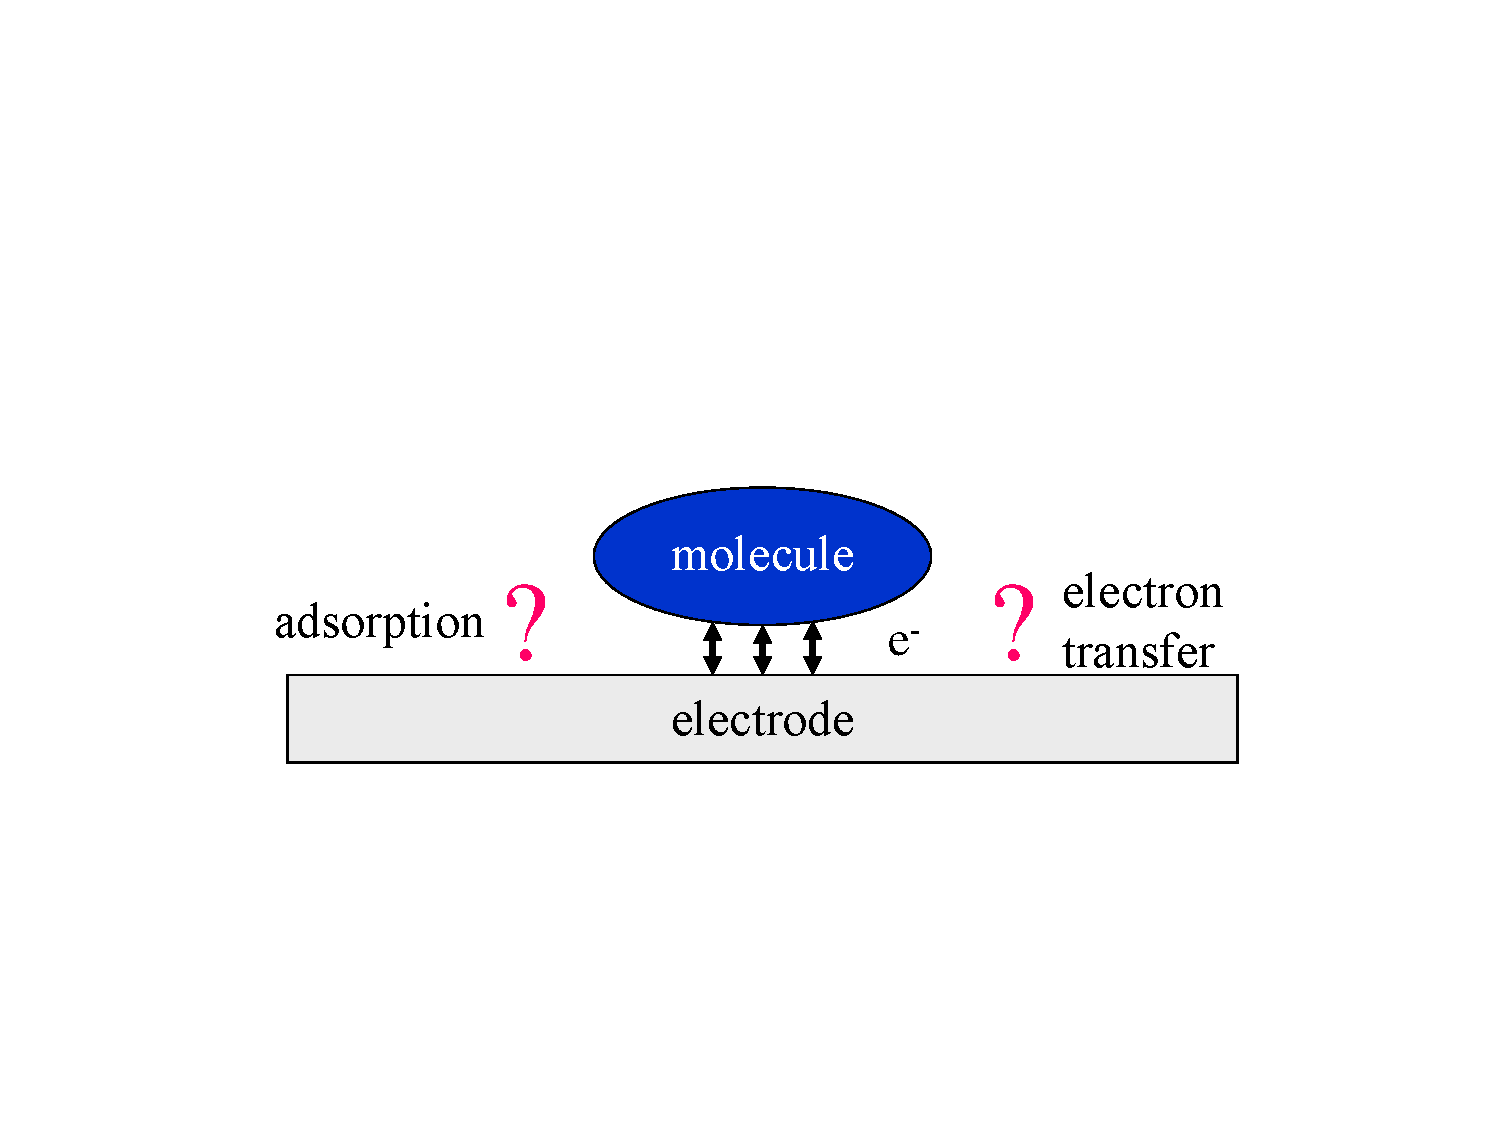
\includegraphics[width=.5\columnwidth]{Electrical_Biosensor}
%%%%%%%%%%%%%%%%%%%%%%%%%%%%%%%%%%%%%%%%%%%%%%%%%%%%%%
\subsection{Transition State Theory \textnormal{$A+B \to [AB] \to C+D$}}
%
%	Criterion is that colliding molecules must have sufficient energy to overcome a potential energy barrier (the activation energy) to react.
%
\formula{Gibbs free energy}{G = H - TS = U + pV - TS}
\formbox{\textbf{Ideal gas law}}{pV = n\ped{total}RT}
\vspace{-1mm}
%%%%%%%%%%%%%%%%%%%%%%%%%%%%%%%%%%%%%%%%%%%%%%%%%%%%%%
\subsubsection{Marcus Theory}
%
\begin{minipage}{.5\columnwidth}
    \includegraphics[width=.8\columnwidth]{Electrochemistry_Marcus_Theory}
\end{minipage}%
\begin{minipage}{.5\columnwidth}
    See \textbf{section \ref{sec:butler-volmer}} (Butler-Volmer)\par
    \begin{tabular}{r@{$\;=\;$}l}
        $k\ped{red}$	& $v\ped{red} \; \eu^{-\frac{\Delta^\ddagger G\ped{red}}{RT}}$\\
        $k\ped{ox}$		& $v\ped{ox}  \; \eu^{-\frac{\Delta^\ddagger G\ped{ox}}{RT}}$\\
        \addlinespace
        $\Delta^\ddagger G\ped{red}$	& $\!\!~^\ddagger G-G\ped{ox,min}$\\
        $\Delta^\ddagger G\ped{ox}$	& $\!\!~^\ddagger G-G\ped{red,min}$
    \end{tabular}
\end{minipage}
%
%	\formula{rate constant}{k_{et} \propto \eu^{-\frac{\Delta^\ddagger G}{RT}}}
%		\quad with \quad $R = k_B N_A = \unit[8.3]{J\;K^{-1}mol^{-1}}$
%%%%%%%%%%%%%%%%%%%%%%%%%%%%%%%%%%%%%%%%%%%%%%%%%%%%%%
\subsubsection{Gerischer's view}
%
\begin{minipage}{.4\columnwidth}
    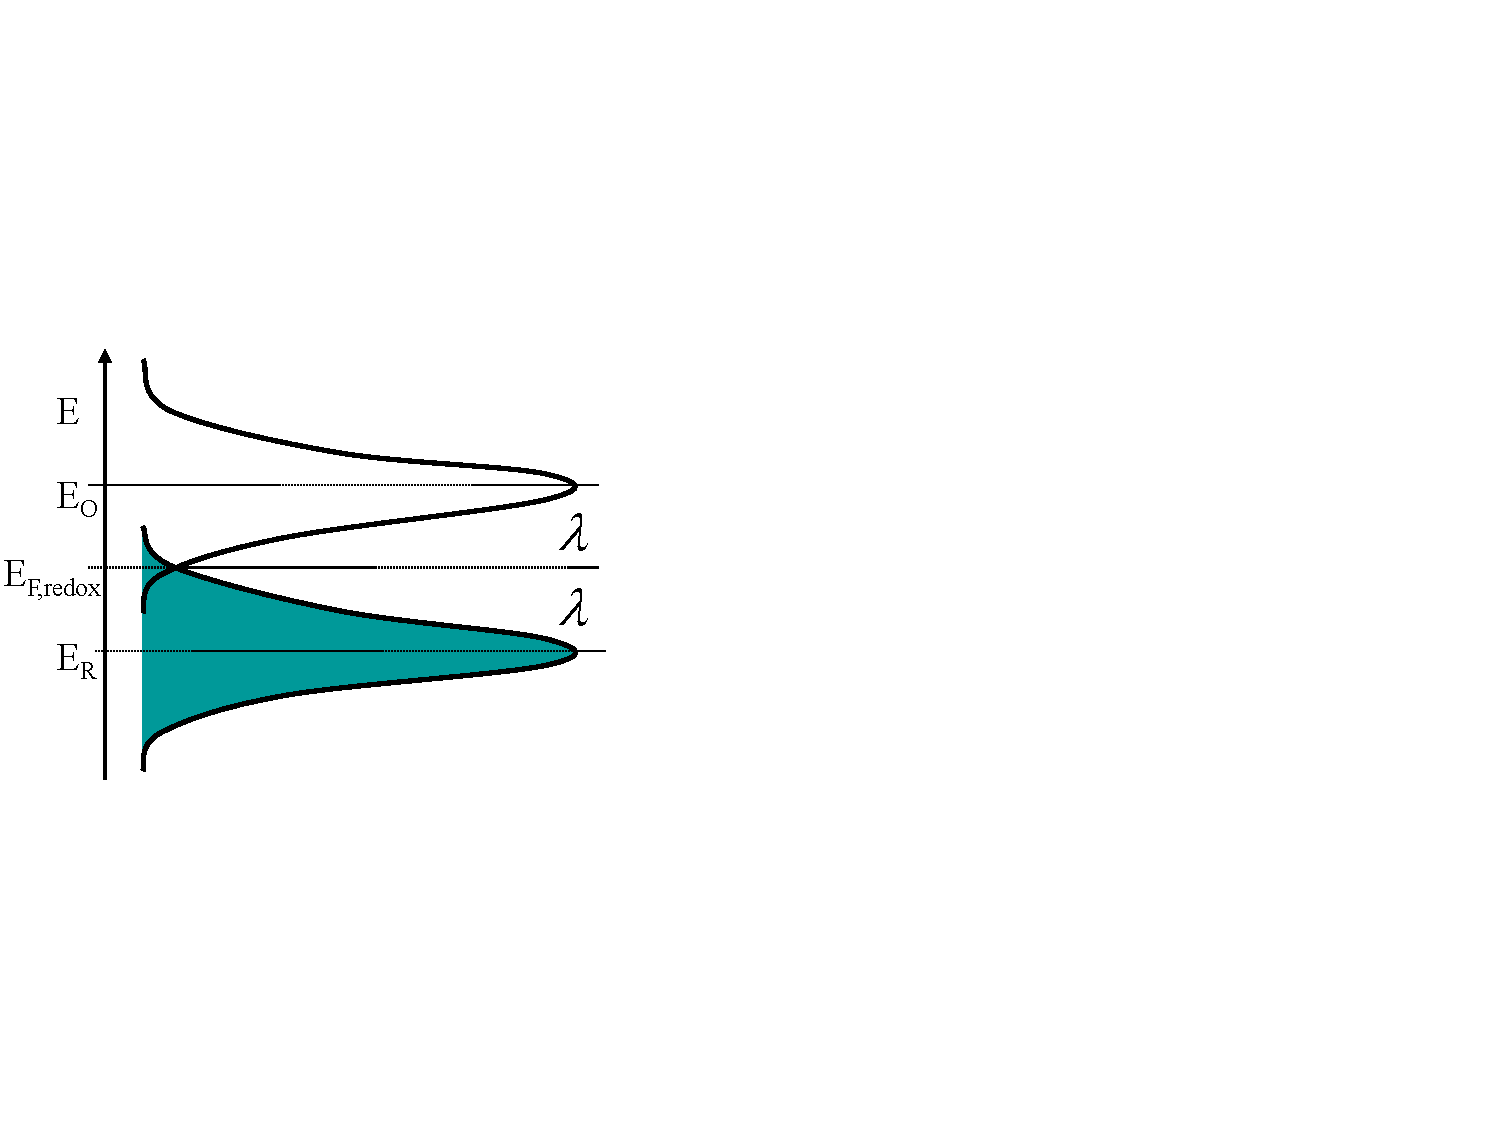
\includegraphics[width=\columnwidth]{Redox_Energy_Levels_1}%
    \hspace{-.6\columnwidth}
    \parbox[b]{.4\columnwidth}{
        $D\ped{ox}(\lambda,E)$ \vspace{20mm}\\\vspace{2mm}
        $D\ped{red}(\lambda,E)$
    }
\end{minipage}%
\begin{minipage}{.15\columnwidth}
    \centering
    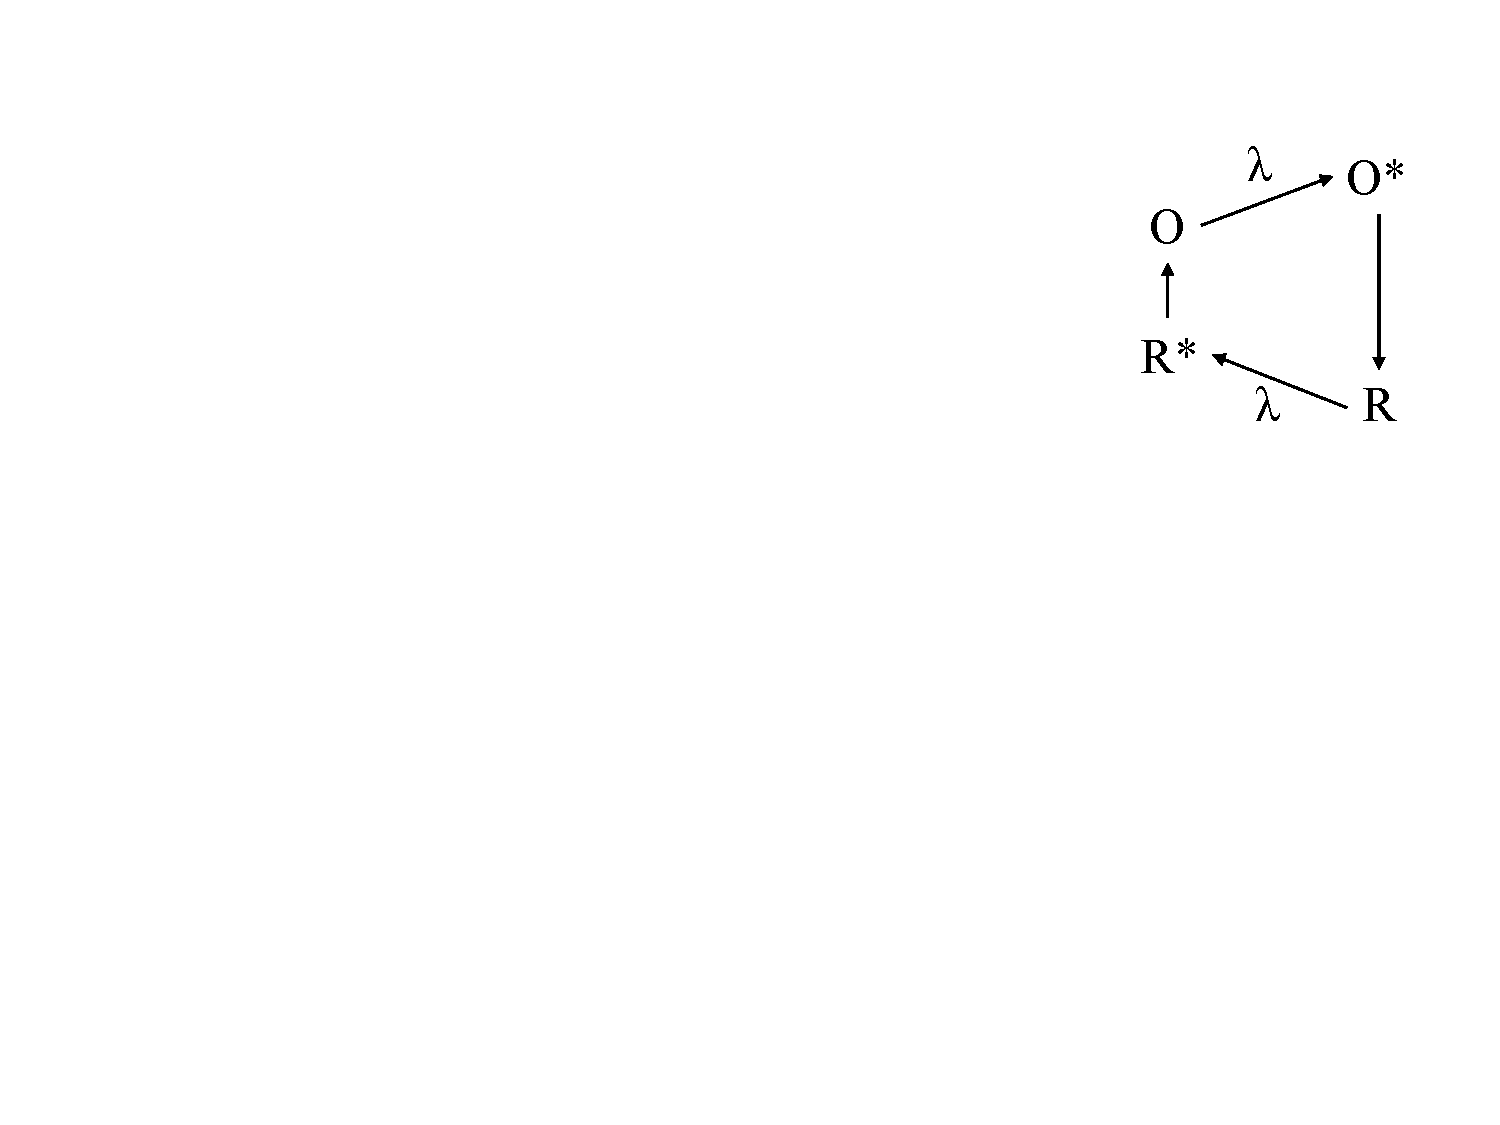
\includegraphics[width=.9\columnwidth]{Redox_Energy_Levels_2}
\end{minipage}%
\begin{minipage}{.45\columnwidth}
    \quad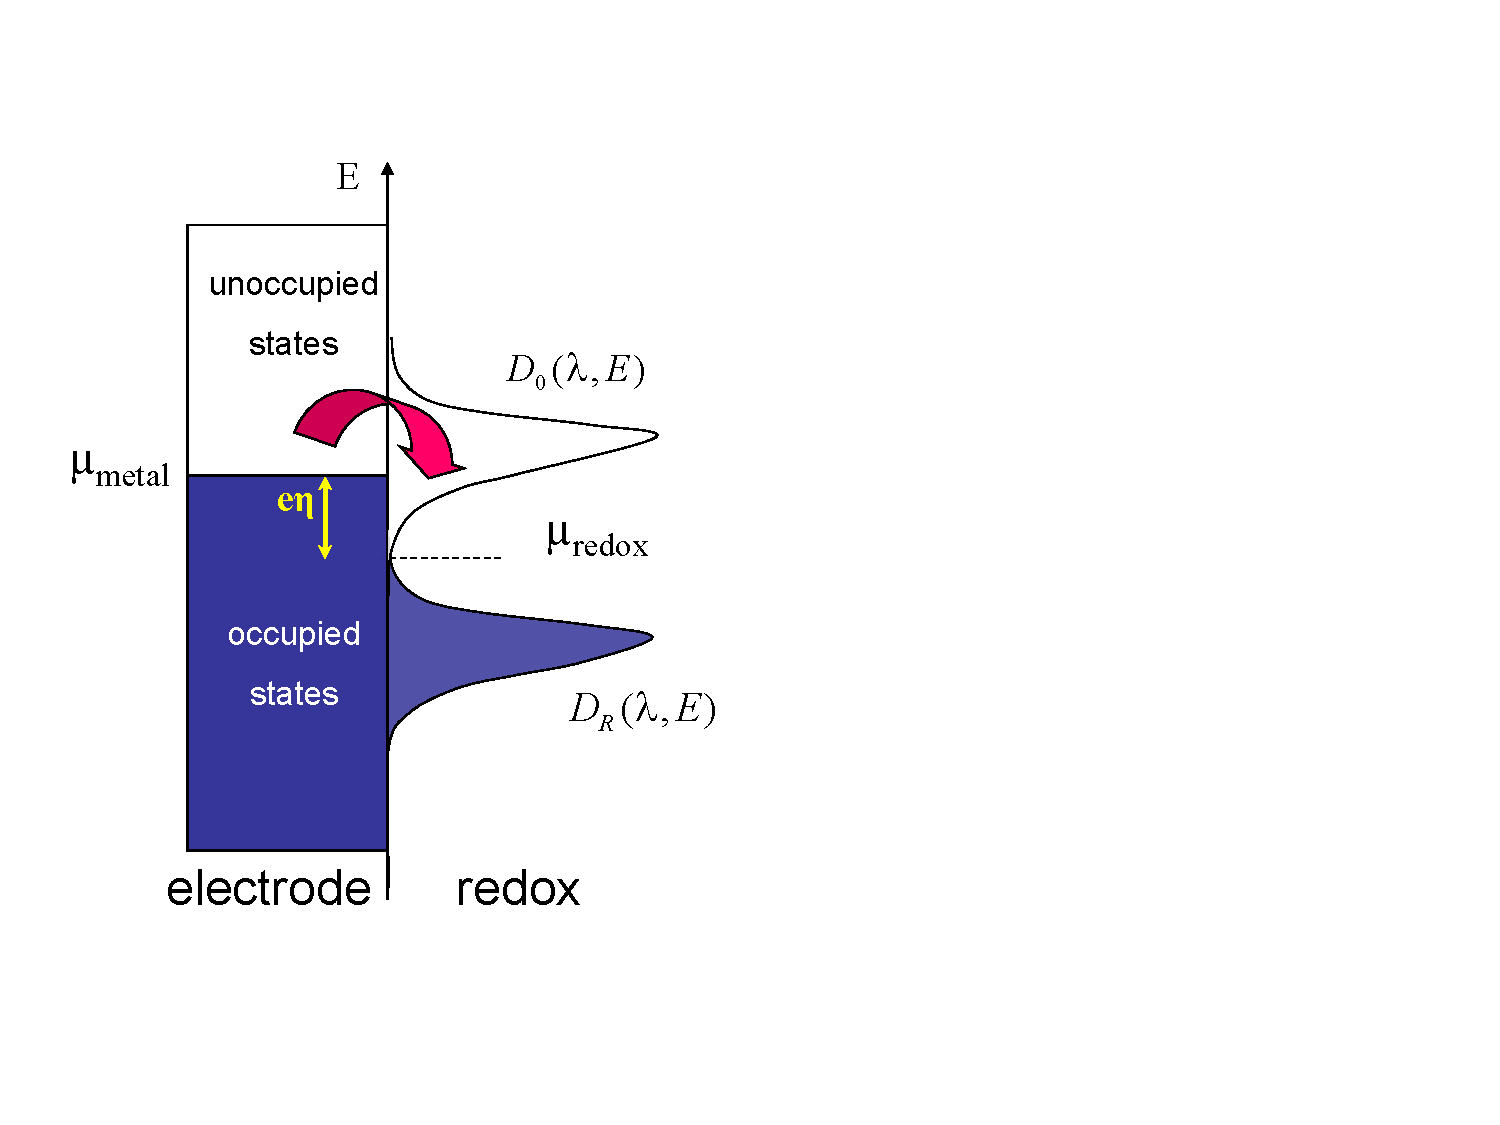
\includegraphics[width=.55\columnwidth]{Electrochemistry_Gerischers_View_Cathodic}%
    \hfill\hspace{-\columnwidth}
    \parbox[b]{\columnwidth}{
        \hfill \textbf{cathodic} polariz. \par
        \hfill $i^+ \gg i^-$\vspace{22mm}\\
    }
%		Gaussian curve: ($+$: red, $-$: ox)\\
%		$W\ped{red/ox} = \frac{1}{\sqrt{4\pi\lambda k\ped{B}T}} \eu^{-\frac{(E-E_F\pm\lambda)^2}{4\lambda k\ped{B}T}}$
\end{minipage}

		%! Author = tstreule

\section{Potentiometric Biosensors}
%%%%%%%%%%%%%%%%%%%%%%%%%%%%%%%%%%%%%%%%%%%%%%%%%%%%%%
%%%%%%%%%%%%%%%%%%%%%%%%%%%%%%%%%%%%%%%%%%%%%%%%%%%%%%
\subsection{Redox Reaction}
%
\textbf{oxidation}: $e^-$ donor (\textit{anode}) \qquad
\textbf{reduction}: $e^-$ acceptor (\textit{cathode})

\formtex{Chemical reaction}{\ce{A*ox + B*X + z*e^- <=>[$k_{red}$][$k_{ox}$] C*red + D*Y}}
\vspace{-.5mm}
\formbox{reaction quotient}{
    Q = \mathrm{\frac{a\ped{ox}^A \;\cdot\; a\ped{X}^B}{a\ped{red}^C \;\cdot\; a\ped{Y}^D}}
}
%\textcolor{gray}{$= \Big(\prod\limits_j a_j^{v_j}\Big)$}
\begin{tabular}{@{$\bullet\;$}l @{\quad$\bullet\;$}l}
    $\mathrm{a}\ped{ion} = r\ped{ion} [\mathrm{ion}]/\unitfrac[1]{mol}{l}$ &
    $\mathrm{a}\ped{solids} = 1$\\
    $\mathrm{a}\ped{gas} = p\ped{gas}/\unit[1.013]{bar}$ &
    $[\ce{H2O}] = 1$
\end{tabular}

\formula{Standard conditions}{
    T = \SI{1}{\degreeCelsius}, \quad
    p = \SI{101.3}{\kilo\pascal} = \SI{1.013}{\bar}
}
\formula{\centering ``STP''}{
    [\mathrm{ion}] \equiv c\ped{ion} = \unitfrac[1]{mol}{l}, \quad
    r = 1 \text{ ``activity coeff.''}
}
%%%%%%%%%%%%%%%%%%%%%%%%%%%%%%%%%%%%%%%%%%%%%%%%%%%%%%
\subsection{Electrochemistry}
%
\formtex{Dynamic equi.}{no net charge over time ($k_1 = k_{-1}$)}
\formula{Chemical potential}{\mu_j = \big( \pderiv{G}{n_j} \big)_{p,T,n'}}
\formula{Equilibrium}{\mu_A = \mu_B}
\quad general: $\sum\limits\ped{prod}v_j\mu_j = \sum\limits\ped{react}v_j\mu_j$
\vspace{-.5mm}
\formula{Chemical potential}{\mu\ped{redox}\equiv E\ped{\emph{F},redox}\equiv E^*}
%\quad where \quad $D\ped{red}(\lambda,E^*) = D\ped{ox}(\lambda,E^*)$
\formbox{Equilibrium}{\bar\mu_A = \bar\mu_B}
\quad $\bar\mu_j = \mu_j^0 + z_jF\Delta\phi$

\formula{\textbf{Contact potential}}{\Delta\phi
    = V\ped{in}-V\ped{out} = \frac{k\ped{B}T}{Q} \ln\left(\frac{[C]\ped{out}}{[C]\ped{in}}\right)
}
\formula{~}{\phantom{\Delta\phi}
    = -\frac{\Delta_rG}{zF}
    = \frac{1}{zF} \Big( \sum\limits\ped{ox} v_j\mu_j - \sum\limits\ped{red} v_j\mu_j + z\mu_e \Big)
}
\formbox{Nernst eq., $\Delta\phi$}{E {=} E^0 {-} \frac{\unit[59]{mV}}{z} \log_{10}Q}
\textcolor{gray}{\footnotesize $\frac{RT}{zF}\ln Q = \frac{2.303 RT}{zF}\log_{10}Q$}
\formtex{~}{$E\ped{cell}=E_1-E_2$ \quad or \quad let $E_1 \overset{!}{=} E_2 \to \mathrm{pH}=\ldots$}
%%%%%%%%%%%%%%%%%%%%%%%%%%%%%%%%%%%%%%%%%%%%%%%%%%%%%%
\subsection{Ion-selective Electrodes \textnormal{(ISE)}}
%
Sensor is seperated to solution through a \ce{H+} permeable glass.
\formbox{pH electrode}{\mathrm{pH} = -\log_{10} a\ped{\ce{H+}} = \frac{K'-\Delta\phi}{\unit[0.059]{V}}}
%%%%%%%%%%%%%%%%%%%%%%%%%%%%%%%%%%%%%%%%%%%%%%%%%%%%%%
\subsection{Bioenzymatic Electrodes}
%
\formtex{Find out how much}{\fbox{\ce{substrate + X + ... ->[enzyme] product + Y + ...}}}
\formtex{of an enzyme was}{Detect \textbf{``a lot''} \ce{X}}
\formtex{initially present}{\hfill$\leftrightarrow$ \textbf{``very few''} \ce{substrate} was initially present}

		%! Author = tstreule

\section{Amperometric Sensors}
%%%%%%%%%%%%%%%%%%%%%%%%%%%%%%%%%%%%%%%%%%%%%%%%%%%%%%
%%%%%%%%%%%%%%%%%%%%%%%%%%%%%%%%%%%%%%%%%%%%%%%%%%%%%%
\subsection{Electrochemistry}
%
\formbox{Overpotential}{\eta \equiv \Delta\phi\ped{appl} {-} \Delta\phi^0 \equiv \phi_s {-} \phi_m \equiv E {-} E^0}
{\hfill\scriptsize $E^0$: Nernst}%
\formula{~}{\eta = 0}
\quad (\textbf{equilibrium} i.e. no net current)

\formula{\textbf{Faraday's law}}{
    \textcolor{gray}{
        \textit{1st: } n\propto Q \textit{,\quad 2nd: } \textrm{(equiv. weigth) } W\ped{eq} = M/z
    }
}
\formbox{\textbf{of electrolysis}}{m = \frac{Q}{z\;F}\;M = \frac{I\;t}{z\;F}\;M = n\cdot M}
\enskip \textcolor{gray}{\scriptsize $[m] {=} \unit{g}$, $[n] {=} \unit{mol}$}
%%%%%%%%%%%%%%%%%%%%%%%%%%%%%%%%%%%%%%%%%%%%%%%%%%%%%%
\subsubsection{Butler-Volmer equation \textnormal{Effect of $\eta$ on barrier heigth $G$}}
\label{sec:butler-volmer}
%
\begin{tabular}{r@{:\quad}l}
    Let
    $\phi_s$	& potential of ions in solution\\
    $\phi_m$	& potential of $e^-$ in (metallic) electrode\\
    $z$			& valency of oxidized species\\
    $n$			& \#of transferred $e^-$\\
    $z-n$		& valency of reduced species
\end{tabular}
\formula{\textbf{transfer coeff. $\alpha$}}{nF\eta = n(1-\alpha)F\eta+n\alpha F\eta}
%		\formula{@equilibrium ($\eta=0$)}{k_0 \equiv k\ped{red}=k\ped{ox}}
\scalebox{.9}{%
    \formbox{\fbox{$f{\equiv}\frac{F}{RT} {\overset{@\unit[298]{K}}{=}} \frac{1}{\SI{25.69}{\milli\volt}}$}}{%
        k\ped{red} {=} k_0\;\eu^{-n\alpha f\eta}, \enskip
        k\ped{ox}  {=} k_0\;\eu^{n(1-\alpha)f\eta}
    }	\shortstack[l]{
        @equi. ($\eta=0$)\\
        $k_0 {\equiv} k\ped{red} {=} k\ped{ox}$
    }
}

The Butler-Vomer eq. relates what we measure (the \textbf{current}) with what we would like to determine (the \textbf{concentration} of an analyte):
\scalebox{.9}{%
    \formbox{\textbf{Butler-Volmer}}{j = \underbrace{nFAk_0\vspace{-1mm}}_{\vspace{-2mm}j_0} \big( C\ped{ox}(0,t)\;\eu^{-\alpha nf\eta} - C\ped{red}(0,t)\;\eu^{(1-\alpha)nf\eta} \big)}}
%%%%%%%%%%%%%%%%%%%%%%%%%%%%%%%%%%%%%%%%%%%%%%%%%%%%%%
\subsection{Cyclic Voltammetry}
%
\begin{minipage}{.4\columnwidth}
    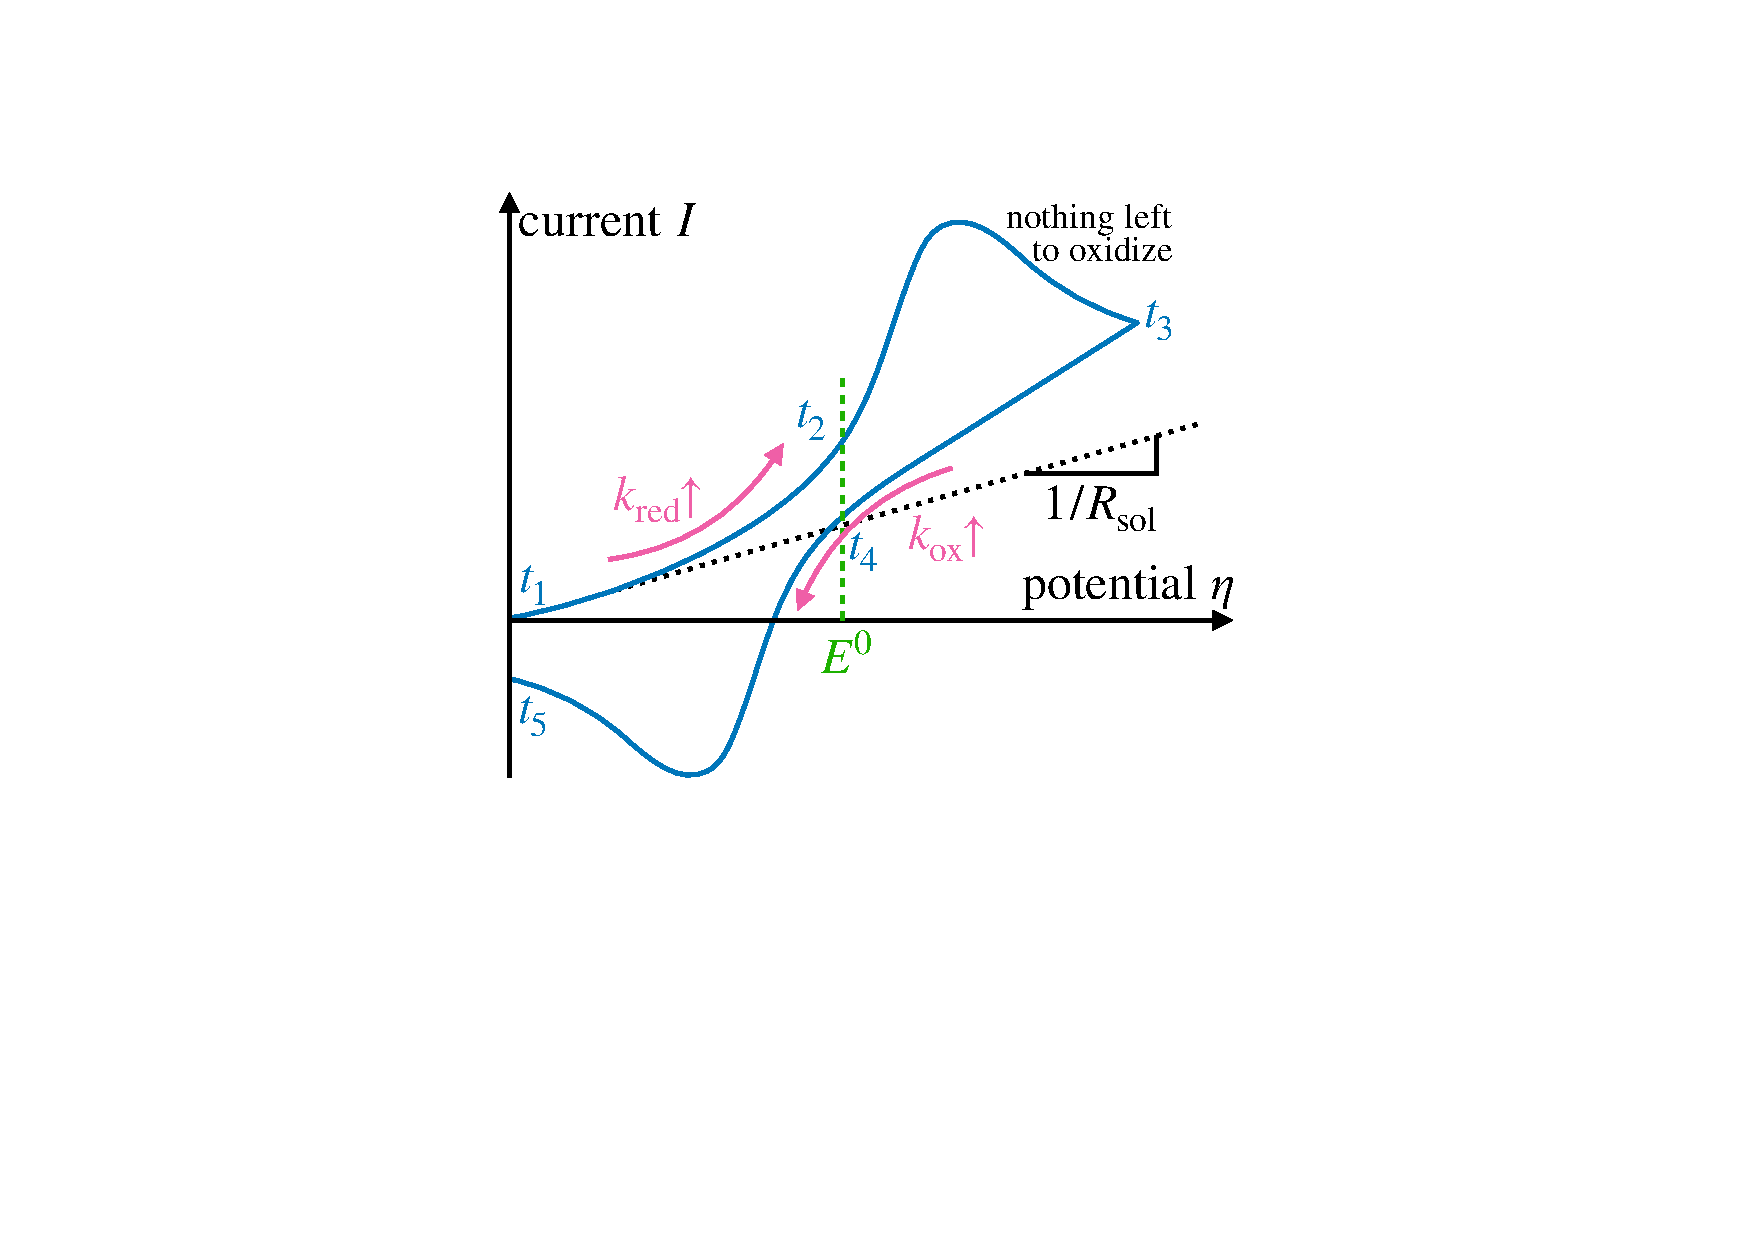
\includegraphics[width=.9\columnwidth]{Electrochemistry_Cyclic_Voltammetry}
\end{minipage}%
\begin{minipage}{.6\columnwidth}
    Offers information on the mechanism of the ec reactions occuring at an electrode.
    \begin{itemize}
        \item May be irreversible\\
        $\to$ \#upper peaks $\neq$ \#lower peaks\\
        $\to$ irreversible reaction fast
        \item Sweep rate\\
        $\to$ irreversible reaction slow
    \end{itemize}
\end{minipage}
\formtex{\textbf{Water electrolysis}}{High potentials/volt's}
%$\to$ affects $I$ %(disturbance, bad)
\formtex{~}{$\to$ affects $I$ (disturbance, bad)}
%%%%%%%%%%%%%%%%%%%%%%%%%%%%%%%%%%%%%%%%%%%%%%%%%%%%%%
\subsection{Amperometric Sensors}
%%%%%%%%%%%%%%%%%%%%%%%%%%%%%%%%%%%%%%%%%%%%%%%%%%%%%%
\subsubsection{Clark \textnormal{(Oxygen)} Electrode \hfill\textnormal{$\to$ Measure \ce{O2}}}
%
\begin{itemize}
    \item test solution \ce{->[O2 passes][membrane]} \ce{Pt} cathode \ce{->[reduction]} current
    \item \ce{Ag} anode is in \ce{KCl} solution ($\to$ ``enough'' \ce{Cl-} for oxidation)
\end{itemize}
%%%%%%%%%%%%%%%%%%%%%%%%%%%%%%%%%%%%%%%%%%%%%%%%%%%%%%
\subsubsection{1st and 2nd Generation}
%
$	\textrm{analyte of interest}
\;\ldots\;
\underbrace{\textrm{redox enzyme}\vspace{-1.5mm}}_{\vspace{-2.5mm}\textrm{catalize}}
\;\underbrace{\ldots\vspace{-.5mm}}_{\vspace{-2.5mm}\textrm{P1}}\;
\underbrace{\textrm{mediator}\vspace{-1mm}}_{\vspace{-2.5mm}\textrm{P2}}
\;\ldots\;
\textrm{Clark Electrode}
$
\formtex{problem P1 (1st)}{\ce{O2} may be consumed, when not measured}
\formtex{problem P2 (2nd)}{need to have ``enough'' of them}
\formtex{Mediator has to be}{$\bullet$ reversible \quad $\bullet$ not toxic \quad $\bullet$ no side reactions}
%%%%%%%%%%%%%%%%%%%%%%%%%%%%%%%%%%%%%%%%%%%%%%%%%%%%%%
\subsubsection{3rd Generation}
%
\textit{Immobilization}/fixation of a redox enzyme on electrode surface

$\to$ free-diffusing redox mediators are not necessary\\
$\to$ in vivo measurments allowed since immobilized

\formtex{problem P3}{Efficient electron transfer (Marcus theory)}\vspace{-1mm}
\formtex{~}{$\to$ may be overcome by mediators}\vspace{-1mm}
\formtex{~}{$\to$ minimize ET distance}
%%%%%%%%%%%%%%%%%%%%%%%%%%%%%%%%%%%%%%%%%%%%%%%%%%%%%%
\subsection{Three Electrode Cell}
%
\begin{minipage}{.5\columnwidth}
    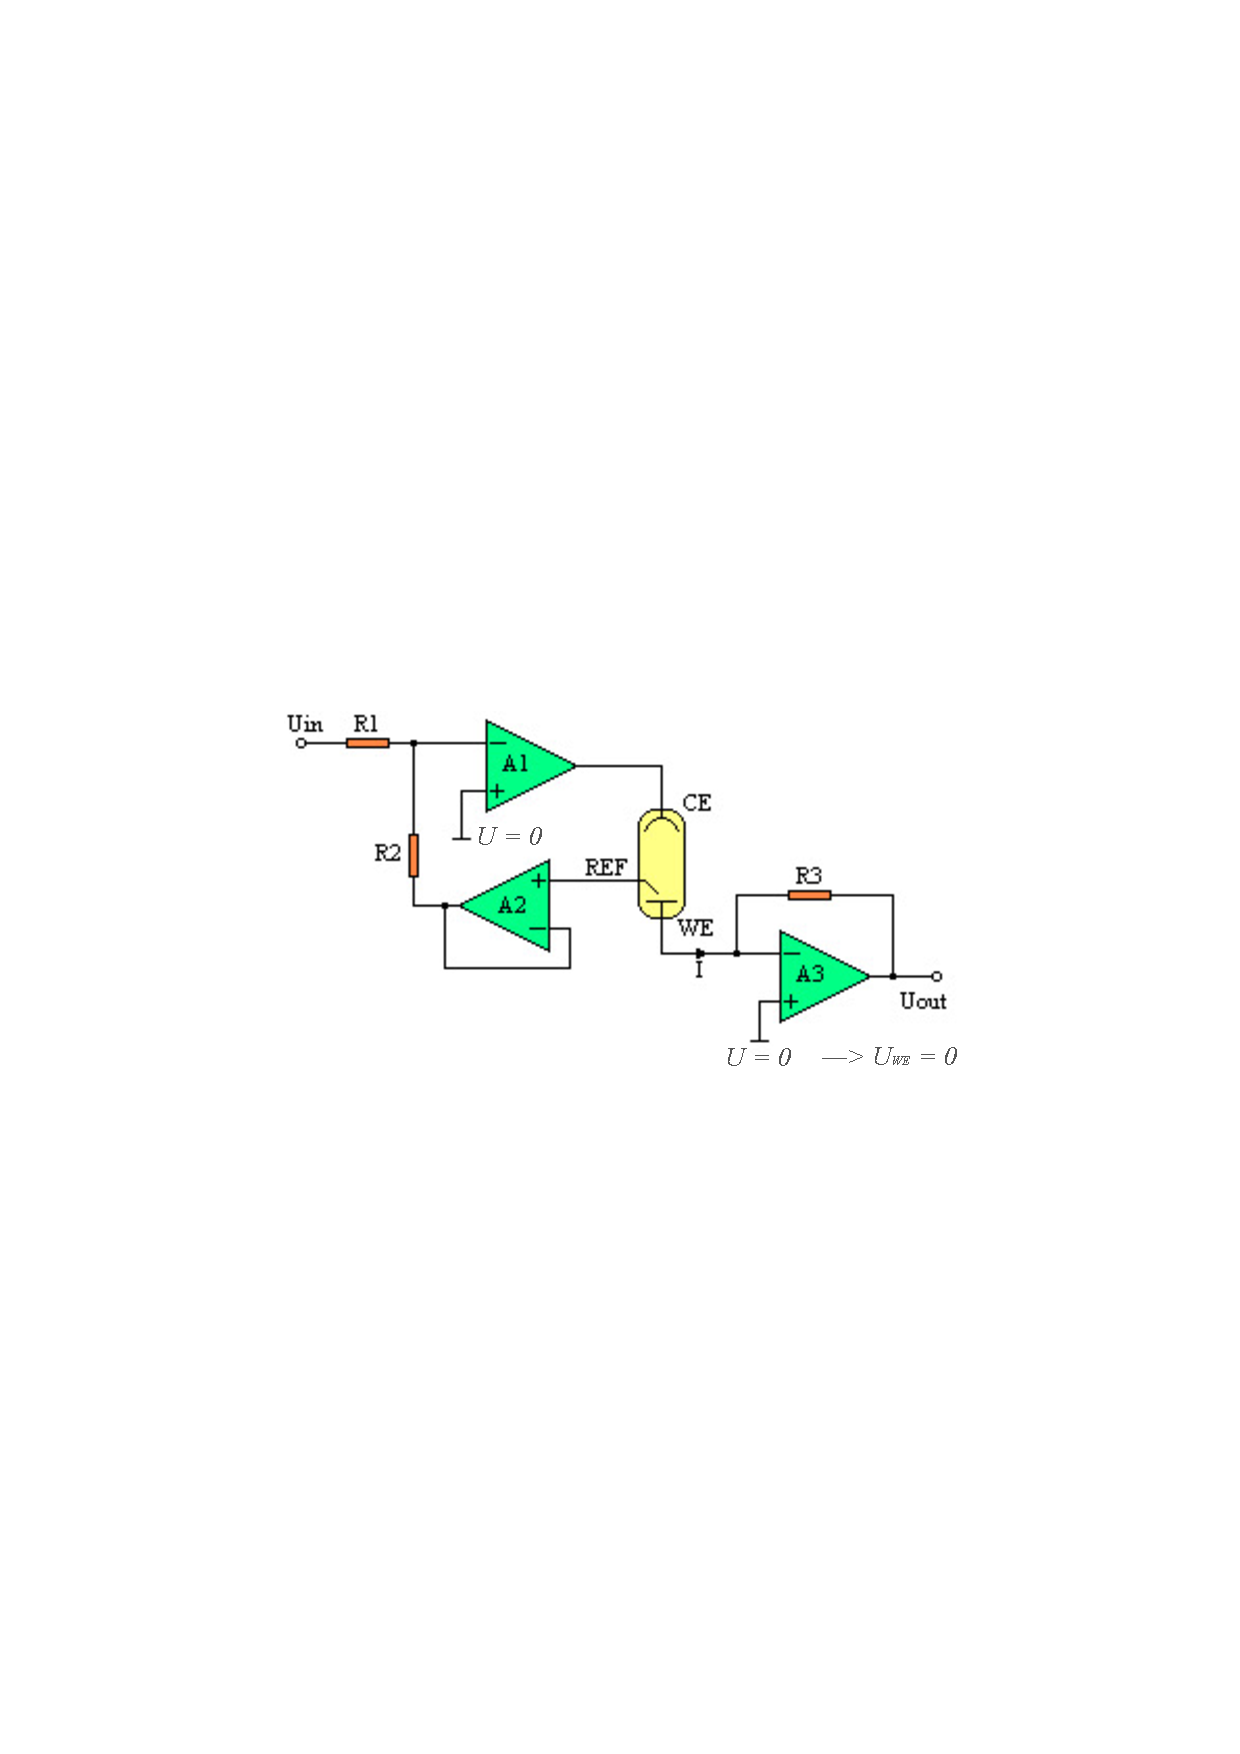
\includegraphics[width=\columnwidth]{Electrochemistry_Three_Electrode_Cell}
\end{minipage}%
\hspace{1cm}
\begin{minipage}{.5\columnwidth-1cm}
    $\frac{U\ped{REF}}{R_2} = - \frac{U\ped{in}}{R_1}$
    \par
    $I = \frac{U\ped{out}}{R_3}$
\end{minipage}

		%! Author = tstreule

\section{Membranes and Transport}
%%%%%%%%%%%%%%%%%%%%%%%%%%%%%%%%%%%%%%%%%%%%%%%%%%%%%%
%%%%%%%%%%%%%%%%%%%%%%%%%%%%%%%%%%%%%%%%%%%%%%%%%%%%%%
\subsection{Diffusion}
%
\formula[\unitfrac{mol}{l}=\unitfrac{mol}{10^3\,cm^3}]{Concentration}{c(x,t)}
\formula[\unitfrac{mol}{cm^2\,s}]{Flux}{\phi(x,t)}

\formbox{\textbf{Fick's law}}{\phi(x,t) = -D_n \pderiv{c_n(x,t)}{x}}
$= \phi_0$ in \textbf{steady state}
\formtex{~}{$D_n$: diffusion coeff $[\unitfrac{cm^2}{s}]$}
\formbox{Continuity eq.}{-\pderiv{\phi_n(x,t)}{x} = \pderiv{c_n(x,t)}{t}}
\formtex{\hfill \vspace{-1mm}e.g.}{\textbf{Delta initial condition} $c(x,t)\vert_{t=0}=n_0\delta(x)$}
\formtex{~}{%
    $c(x,t) {=} \frac{n_0}{\sqrt{2\pi\sigma}} \eu^{-x^2\!/\sigma^2}$,\hfill
    $\sigma {=} \sqrt{2D_nt}$,\hfill
    $t_{\unitfrac{1}{2}} {=} \frac{1}{D_n} x_{\unitfrac{1}{2}}^2$
}
%%%%%%%%%%%%%%%%%%%%%%%%%%%%%%%%%%%%%%%%%%%%%%%%%%%%%%
\subsubsection{Diffusion across membrane}
%
\formtex{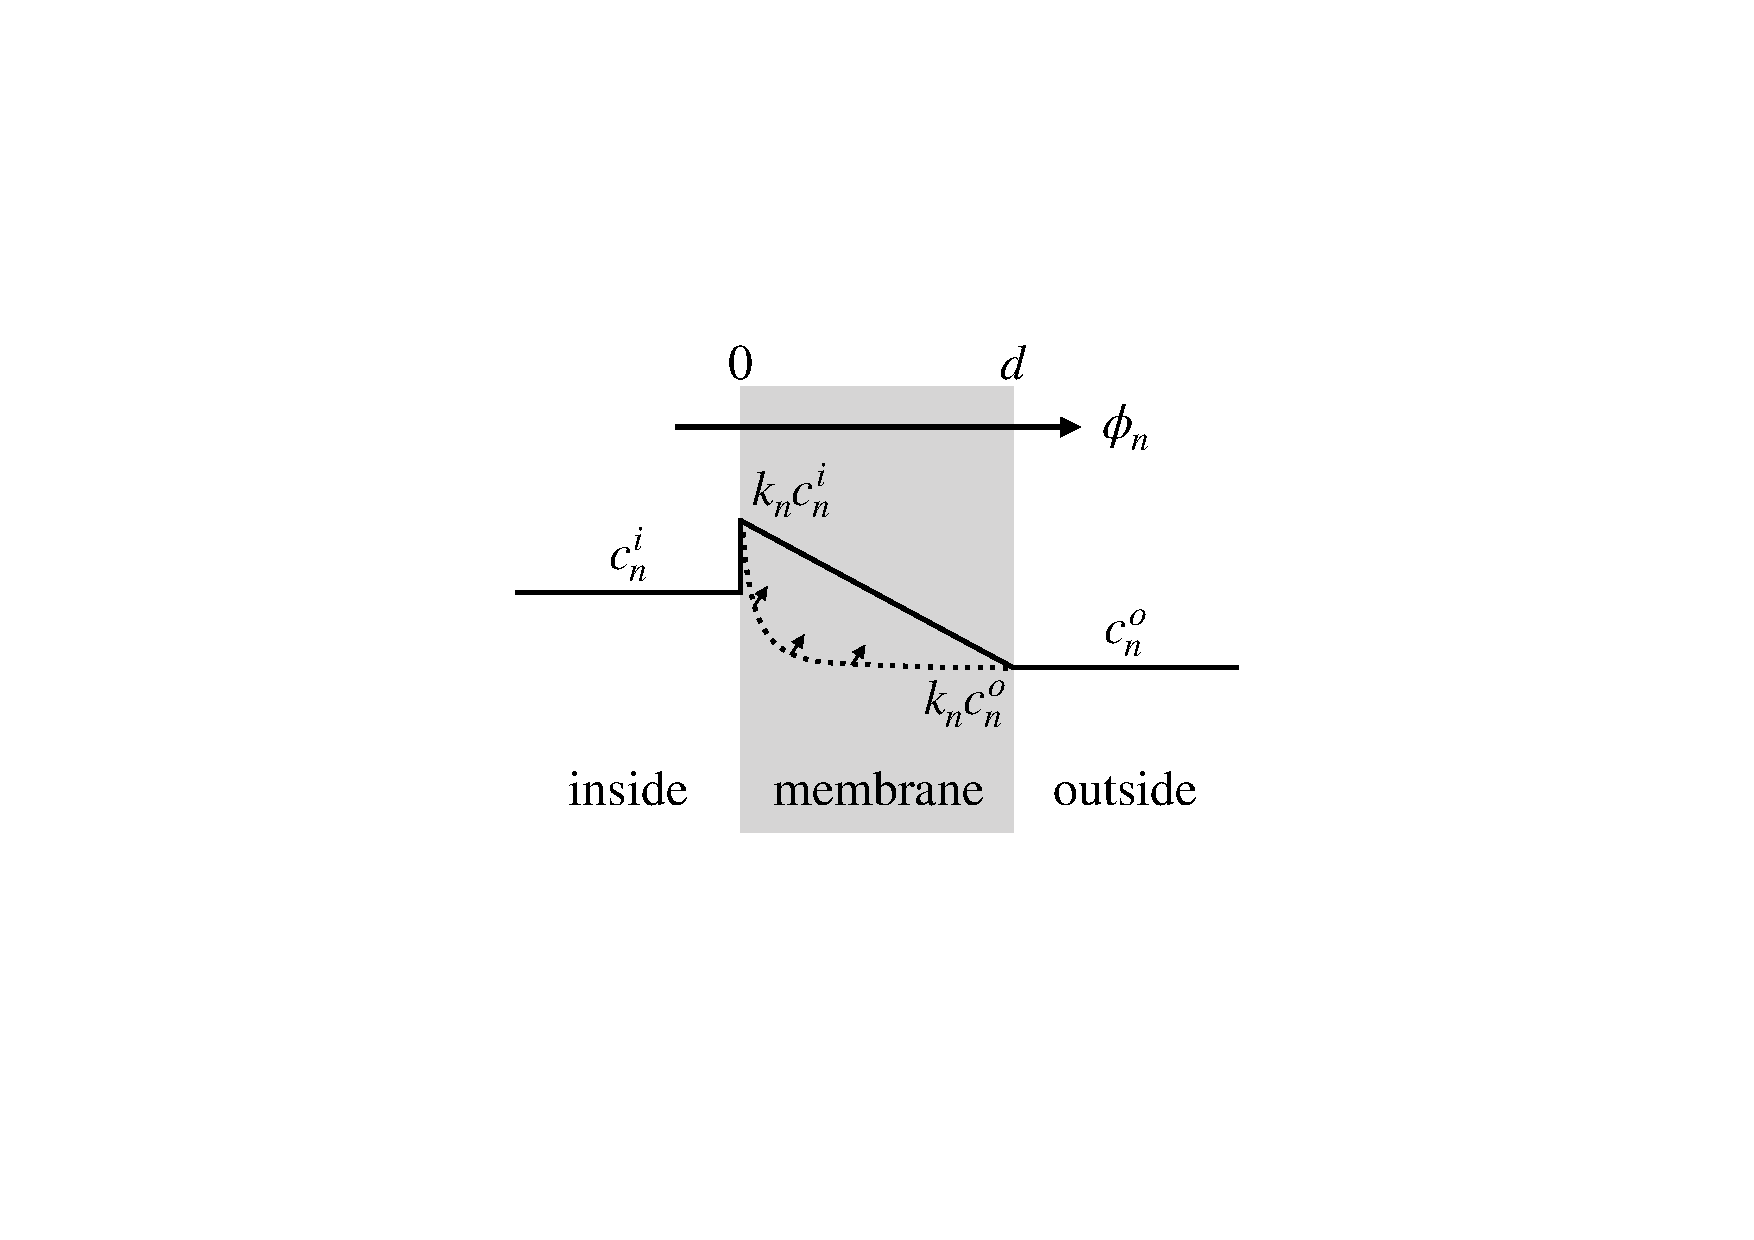
\includegraphics[width=.3\columnwidth]{Transport_Diffusion}}{%
%    \hspace{1cm}%
    \parbox{.7\columnwidth}{%
        $\phi_n(t) = P_n\,(c_n^i(t) - c_n^o(t))$\\
        with permeability: $P_n = \frac{D_nk_n}{d}$\\[1em]
        state space (inside membrane)\\
        after $\tau\ped{SS} = \frac{d^2}{\pi^2D_n}$
    }}
%%%%%%%%%%%%%%%%%%%%%%%%%%%%%%%%%%%%%%%%%%%%%%%%%%%%%%
\subsection{Osmosis}
%
\vspace{-2mm}
\formbox{\vspace{2mm}Osmotic (back-)pressure}{\pi(x,t) = RT\; \sum\limits_n c_n(x,t)}
\vspace{2mm} {\small\enskip $c_\Sigma(x,t)$: \parbox{.2\columnwidth}{osmolarity/\\total conc.}}
\formula{Zero pressure if}{\pi_i - \pi_o = 0}
\formula{Volume of the cell}{v_c(\infty) = v_c' + \frac{N_\Sigma^i}{c_\Sigma^o}}
\quad $v_c'$: non-water volume
%%%%%%%%%%%%%%%%%%%%%%%%%%%%%%%%%%%%%%%%%%%%%%%%%%%%%%
\subsection{Carrier mediated Transport}
%
\formtex{Hints for their}{$\bullet$ Saturation of solute trsp. (\lightning~Fick's law)}
\formtex{existance}{$\bullet$ Competitive inhib. \quad $\bullet$ Structure specificy}

\textbf{4-state carrier model}

\begin{minipage}{.5\columnwidth}
    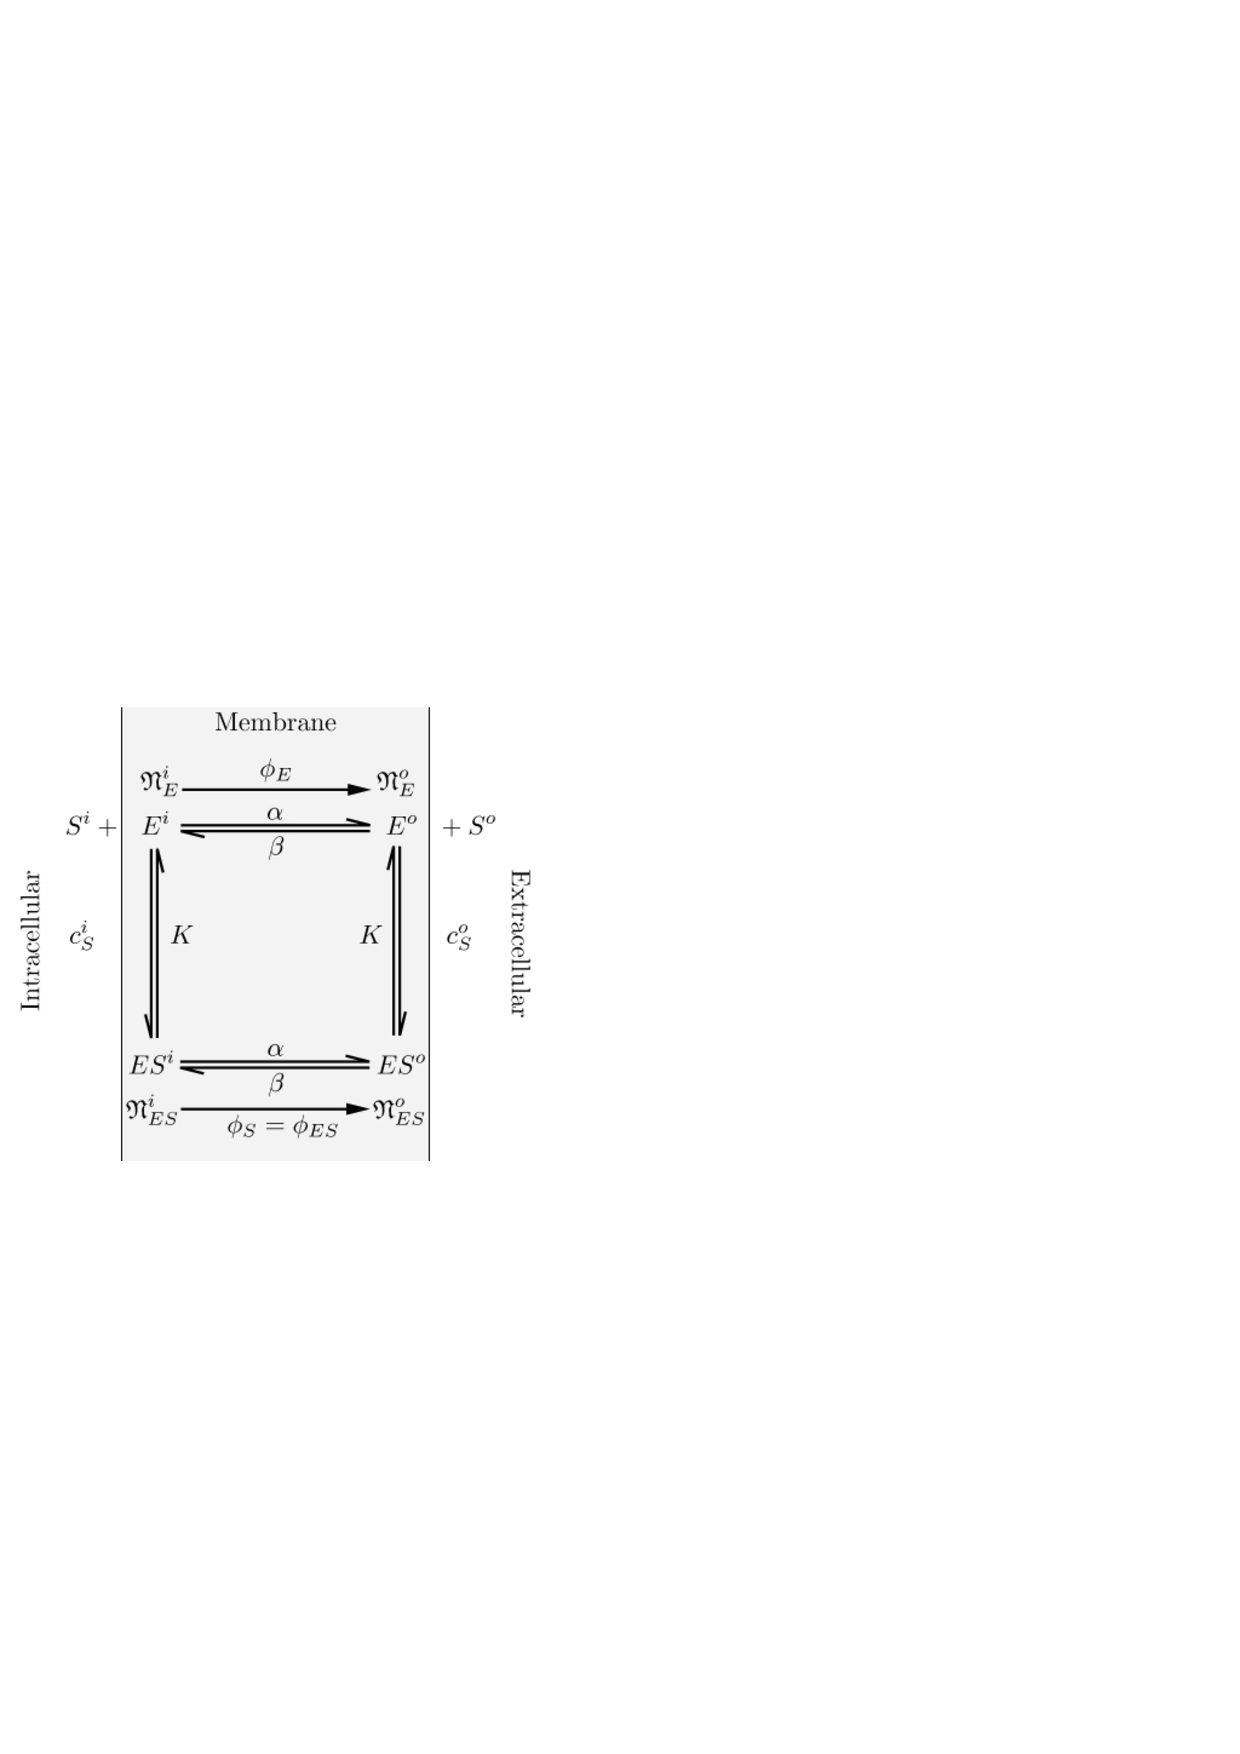
\includegraphics[width=.9\columnwidth]{Transport_Carriers}
\end{minipage}%
\begin{minipage}{.5\columnwidth}
    \begin{enumerate}
        \item Conservation\par
        \quad $N_E^i + N_E^o + N_{ES}^i + N_{ES}^o = N_{ET}$
        \item Fast binding (always steady state)\par
        \quad $K = \frac{c_S^i N_E^i}{N_{ES}^i} = \frac{c_S^o N_E^o}{N_{ES}^o}$
        \item Translocation (char. by flux)\par
        \quad $\phi_{E(S)} = \alpha N_{E(S)}^i - \beta N_{E(S)}^o$
        \item Zero net flux\par
        \quad $\phi_E + \underbrace{\phi_{ES} \vspace{-1mm}}_{\phi_S} = 0$
    \end{enumerate}
\end{minipage}
\scalebox{.9}{
    \formula{Net flux \underline{out} of cell}{\phi_S {=} \frac{\alpha\beta}{\alpha+\beta}N_{ET} \paren*{\frac{c_s^i}{c_s^i + K} {-} \frac{c_s^o}{c_s^o + K}}
    \enskip (\phi_S)\ped{max} {=} \frac{\alpha\beta}{\alpha+\beta}N_{ET}}}
%%%%%%%%%%%%%%%%%%%%%%%%%%%%%%%%%%%%%%%%%%%%%%%%%%%%%%
\subsection{Ion Transport}
%
\formbox{\textbf{Continuity eq.}}{\pderiv{J_n(x,t)}{x} = -z_n F \pderiv{c_n(x,t)}{t}}
\enskip $z_n$: valency
\formbox{\textbf{Poisson eq.}}{\pderiv[2]{\psi(x,t)}{x} = -\frac{1}{\epsilon} \sum_n z_nFc_n(x,t)}
\formtex{\centering i.e.}{electric field potential = local charge density}
\formbox{\vspace{3mm}\textbf{Nernst-Planck eq.}\\$u_n$: molar mobility}{\scriptsize
    \underbrace{J_n(x,t) \vspace{-1mm}}_\mathrm{current}
    =- \underbrace{z_nFD_n\pderiv{c_n(x,t)}{x} \vspace{-1mm}}_\textrm{diffusion of charge}
    - \underbrace{u_nz_n^2F^2c_n(x,t)\pderiv{\psi(x,t)}{x} \vspace{-1mm}}_\textrm{mobility of charge in E-field}
}

Debye Length ``depletion width'': $\lambda_D \simeq \unit[1]{nm}$ within $\tau_r \simeq \unit[1]{ns}$
\formbox{\textbf{Nernst Equi. Pot.}}{V_n = \frac{\unit[59]{mV}}{z_n} \log_{10}Q}
\enskip with
\enskip \highlight{$\!\!\textstyle Q = \frac{c_s^o}{c_s^i}\!\!$},
\enskip $\frac{D_n}{u_n} = RT$
\formula{~}{V\ped{K} \simeq \unit[-75]{mV}, \quad V\ped{Na} \simeq \unit[55]{mV}}
\formula{Donnan equil.}{V_m {=} V_n \Rightarrow I_n=0}
\textcolor{gray}{\enskip $\left(\frac{c_n^o}{c_n^i}\right)^{\pm\frac{1}{z_n}} {=} \eu^\frac{FV_m}{RT}$, $+$: anodic}
%%%%%%%%%%%%%%%%%%%%%%%%%%%%%%%%%%%%%%%%%%%%%%%%%%%%%%
\subsubsection{Resting (membrane) potential}
%
\begin{minipage}{.35\columnwidth}
    \centering
    Resting $\leftrightarrow$ $I_m = 0$\par
    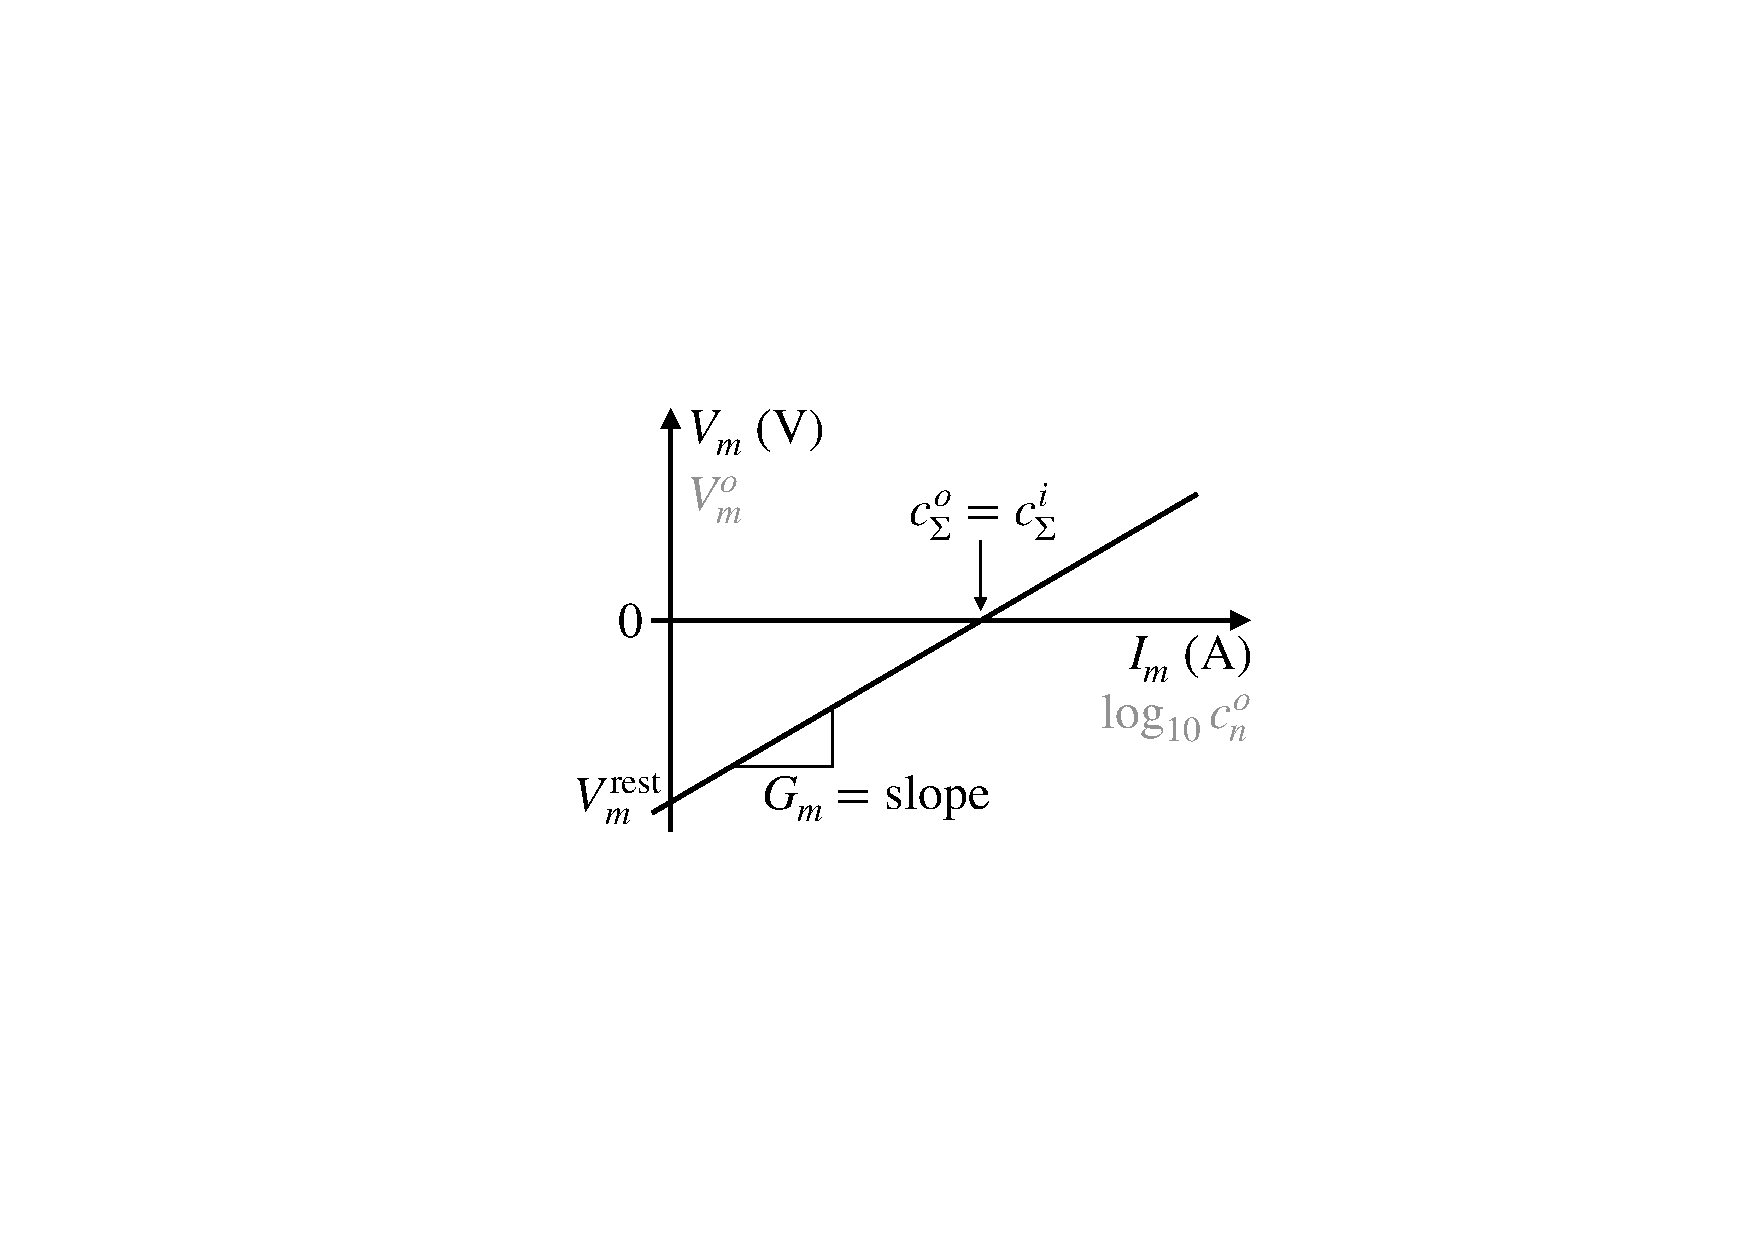
\includegraphics[width=\columnwidth]{Transport_Resting}
\end{minipage}
\hfill
\begin{minipage}{.25\columnwidth}
    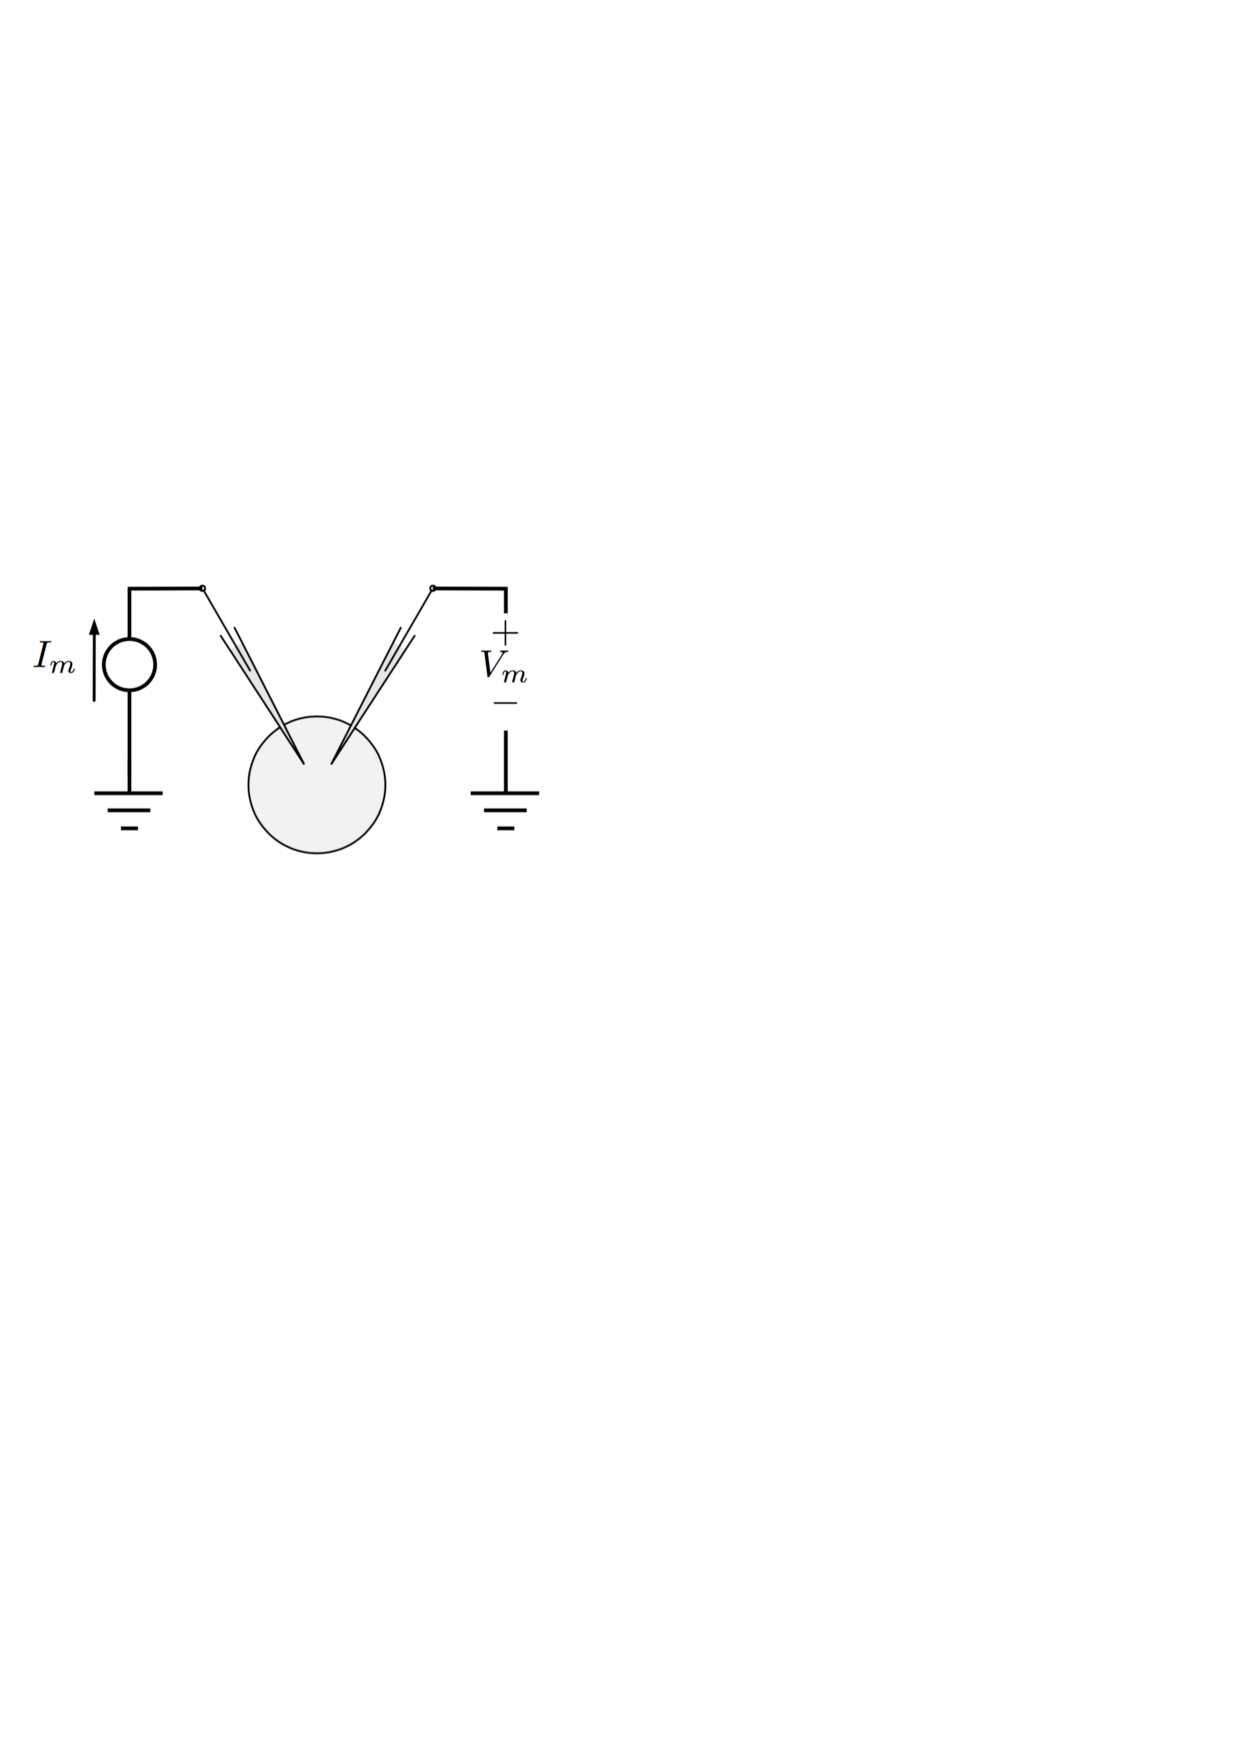
\includegraphics[width=\columnwidth]{Transport_Current}
\end{minipage}
\hfill
\begin{minipage}{.35\columnwidth}
    \includegraphics[width=\columnwidth]{Transport_Multiple_Ion}
\end{minipage}

\formtex{\textbf{3-ion model}}{permeable to \ce{K}, \ce{Na} and some others}
\formbox{Resting potential}{V_m\ap{rest} {=} \frac{V\ped{K}\;G\ped{K}}{G\ped{tot}} {+} \frac{V\ped{Na}\;G\ped{Na}}{G\ped{tot}} {+} \frac{V_o\;G_o}{G\ped{tot}}}
{\scriptsize $G\ped{tot} {\equiv} G_m {=} \mathrm{slope}$}
\formtex{$J_m = J\ped{K} \!+\! J\ped{Na} \!+\! J_o = 0$}{where $J_n\!\neq\!0$ (only momentarly rest)}
%%%%%%%%%%%%%%%%%%%%%%%%%%%%%%%%%%%%%%%%%%%%%%%%%%%%%%
\subsection{Active Transport}
%
Rest is only momentarly $\to$ maintain conc. grad with \textit{act. transport}
\begin{itemize}
    \item Ions moving against its conc. gradient $\to$ ATP needed
    \item Active pumps for $J_m\!=\!0$ (rest) and $J_{n,\mathrm{in}} \!+\! J_{n,\mathrm{out}} = 0$ (quasi equilib.)
\end{itemize}

		%! Author = tstreule

\section{Action Potential \& Hodgkin-Huxley Model}
%%%%%%%%%%%%%%%%%%%%%%%%%%%%%%%%%%%%%%%%%%%%%%%%%%%%%%
%%%%%%%%%%%%%%%%%%%%%%%%%%%%%%%%%%%%%%%%%%%%%%%%%%%%%%
\begin{minipage}[t]{.5\columnwidth-.5\columnsep}
    \subsection{Current Clamp}
    %
    \textbf{Fix current} $I_m$ and\\
    measure membrane potential
    \begin{itemize}
        \item[$\to\!\!$] Good for observing AP\\
        (since voltage can change)
    \end{itemize}
\end{minipage}%
\hspace{\columnsep}%
\begin{minipage}[t]{.5\columnwidth-.5\columnsep}
    \subsection{Voltage Clamp}
    %
    \textbf{Fix voltage} $V_m$ and\\
    measure the current
    \begin{itemize}
        \item[$\to\!\!$] Good for studying membrane channel proteins (ion transp.)
    \end{itemize}
\end{minipage}
%%%%%%%%%%%%%%%%%%%%%%%%%%%%%%%%%%%%%%%%%%%%%%%%%%%%%%
\subsection{2-state ion channel model}
%
\formula{two states}{\ce{close <=>[\alpha][\beta] open}}
\quad with gate charge $Q$
\formula{\#open states}{\deriv{n(t)}{t} = \alpha (\mathcal{N} - n(t)) - \beta n(t)}
\formbox{Prob. being open}{x(t) \simeq \frac{n(t)}{\mathcal{N}} = x_\infty\! + (x_0-x_\infty\!) \;\eu^{-t/\tau_x}}
\formbox{~}{x_\infty\! = \frac{\alpha}{\alpha+\beta}, \quad \tau_x = \frac{1}{\alpha+\beta}}

\begin{minipage}{\linewidth}
    \begin{minipage}{\linewidth}
        \formula{Boltzmann law}{\alpha = A\;\eu^{(E_c-E_B)/kT}}
        \formula{~}{\beta = A\;\eu^{(E_o-E_B)/kT}}
        \formula{~}{x_\infty\! = \frac{1}{1+\beta/\alpha} = \frac{1}{1+\eu^{-QV_m/kT}}}
        \formula{~}{\tau_x = \frac{1}{A\;\eu^{-\frac{1}{2}QV_B/kT}} \cdots}
        \formula{~}{\phantom{\tau_x =} \cdots \frac{1}{\eu^{\frac{1}{2}QV_m/kT} + \eu^{-\frac{1}{2}QV_m/kT}}}
    \end{minipage}
    \begin{minipage}{\linewidth}
        \vspace{-30mm}\hfill
        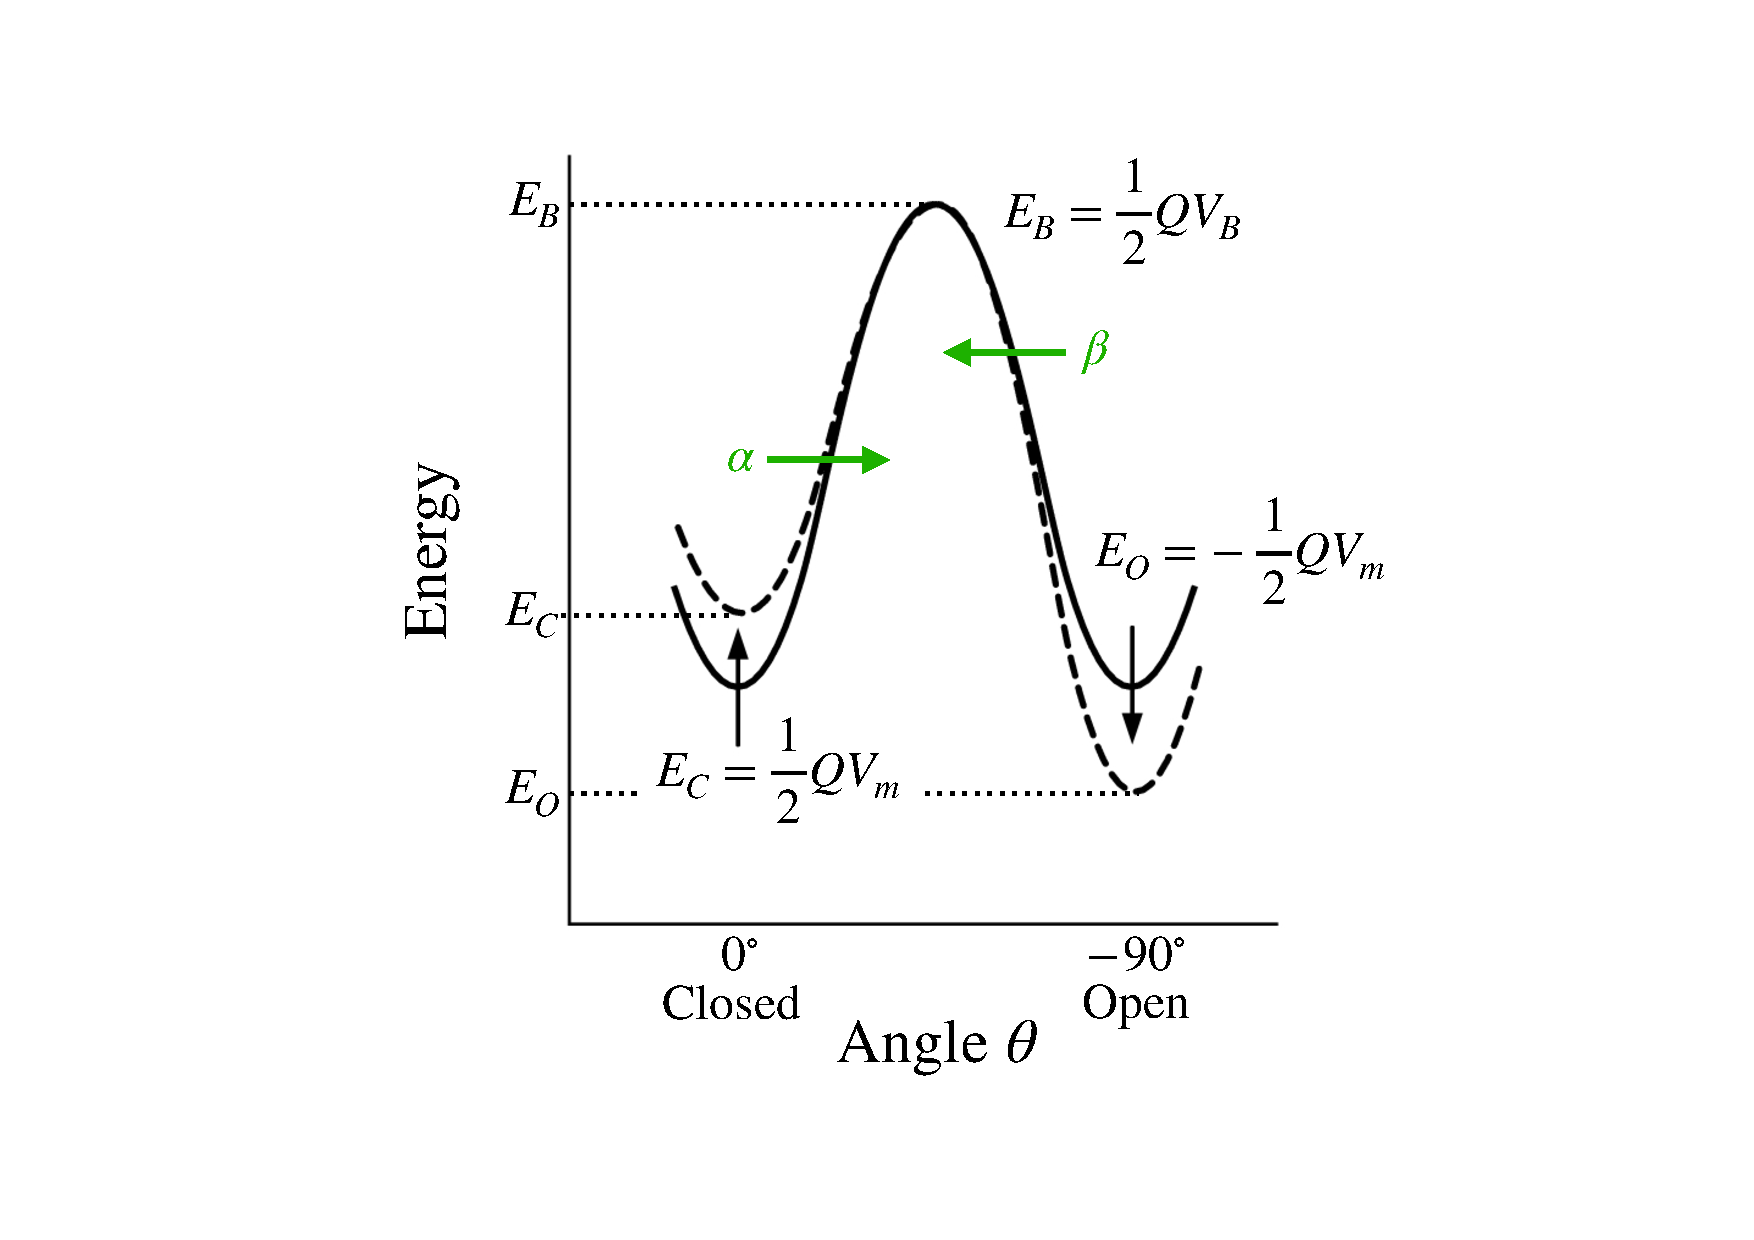
\includegraphics[width=.35\columnwidth]{AP_Boltzmann}
    \end{minipage}
\end{minipage}
%%%%%%%%%%%%%%%%%%%%%%%%%%%%%%%%%%%%%%%%%%%%%%%%%%%%%%
\subsection{Circuit Model \textnormal{(Conductance) \hfill\small$V\ped{K} \simeq \unit[-75]{mV}, \quad V\ped{Na} \simeq \unit[+55]{mV}$}}
%
\formtex{~}{\scalebox{.9}{%
    \highlight{$J\ped{C} = C_m \deriv{V_m(t)}{t}$} \enskip \fbox{$J_m = C_m \deriv{V_m}{t} + G_m(V_m-V_m\ap{rest})$}}}
\formtex{~}{\scalebox{.9}{%
    \highlight{$J\ped{K} = G\ped{K}\;(V_m-V\ped{K})$} \scriptsize always $>0$, we don't fall below ($V_m>V\ped{K}$)}}
\formtex{~}{\scalebox{.9}{%
    \highlight{$J\ped{Na} = G\ped{Na}\;(V_m-V\ped{Na})$} \scriptsize $\begin{cases}>0 & \text{if } V_m-V\ped{Na}>0 \\ <0 & \text{otw.} \end{cases}$}}

\vspace{-18mm}%
\begin{minipage}{\linewidth}
    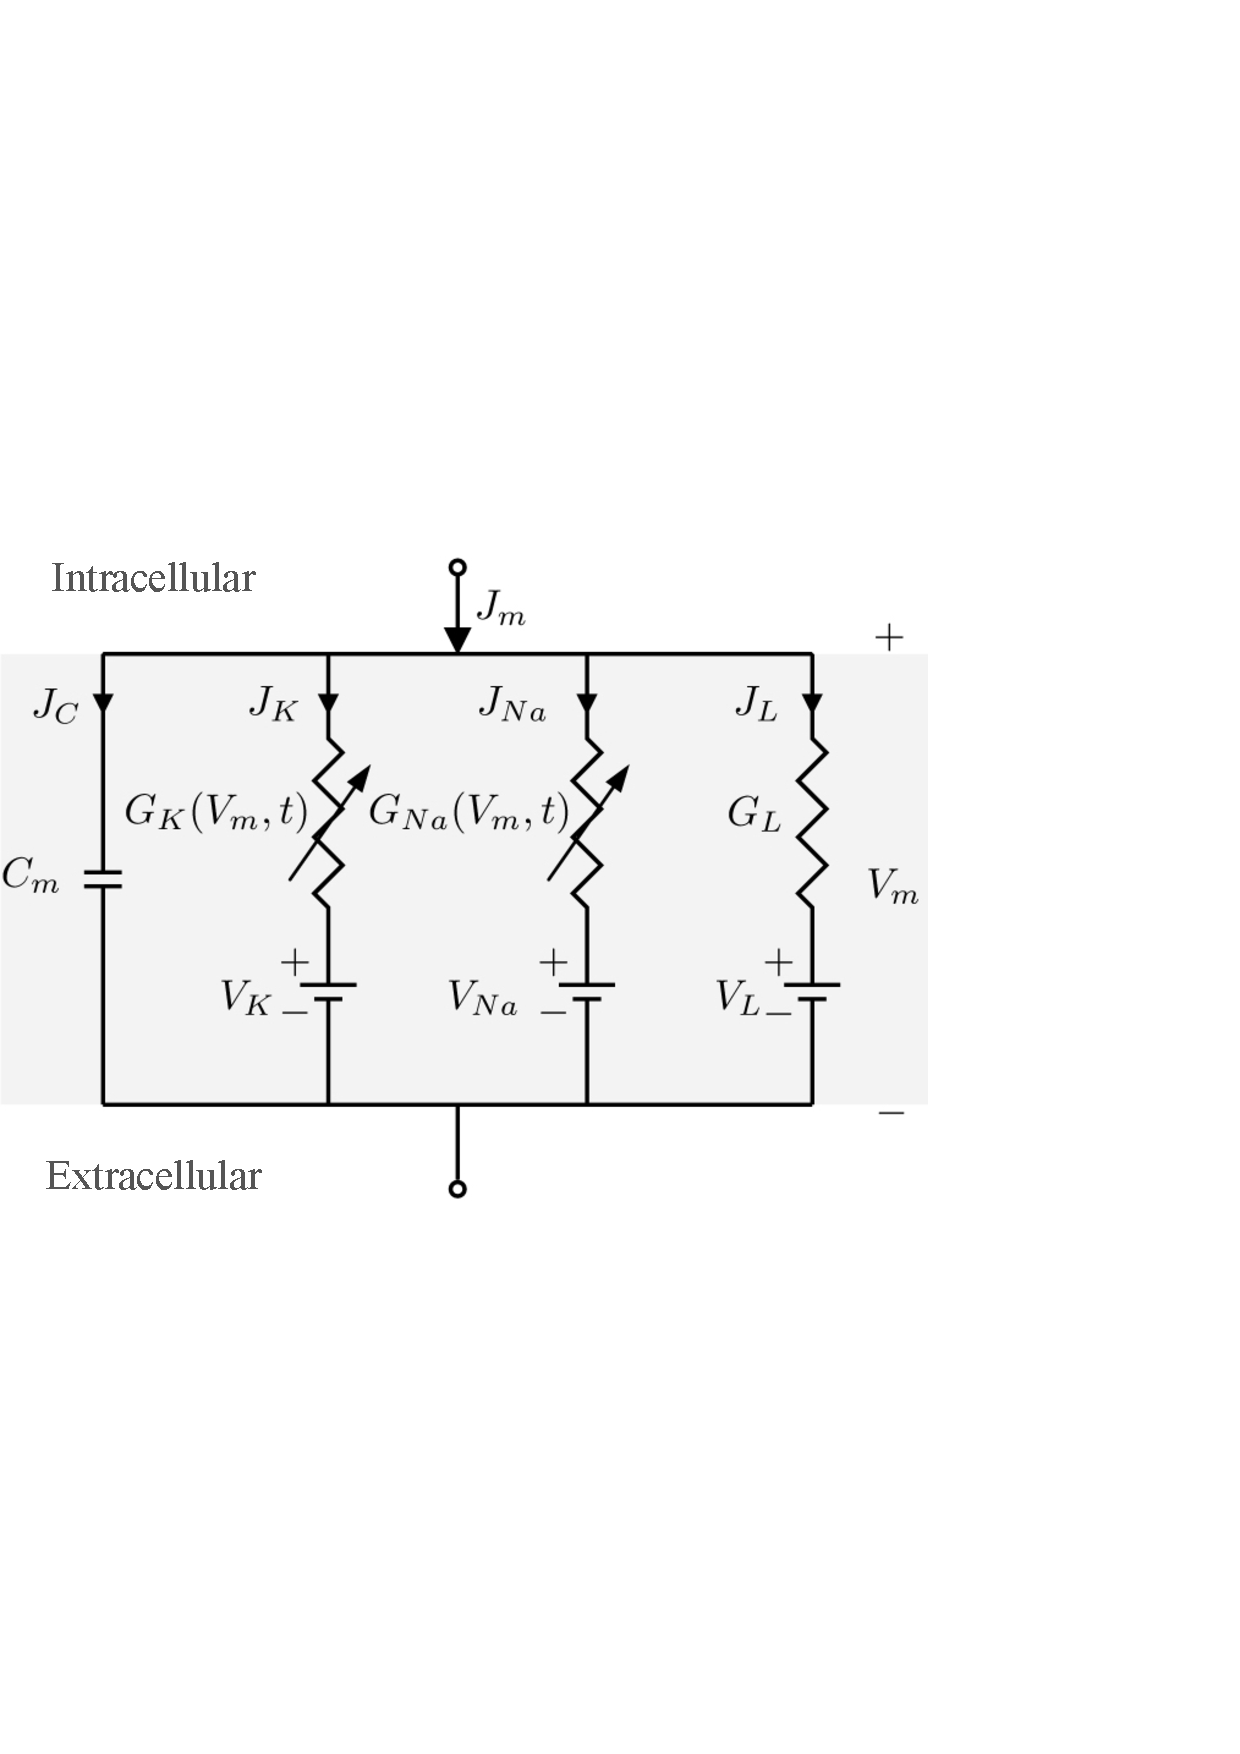
\includegraphics[width=.3\columnwidth]{AP_Conductance_Model}
\end{minipage}

\begin{minipage}{.25\columnwidth}
    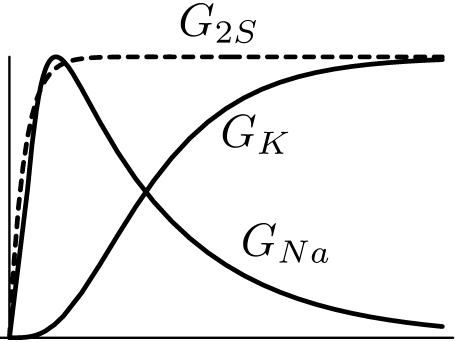
\includegraphics[width=.8\columnwidth]{AP_Conductance}
\end{minipage}
\begin{minipage}{.75\columnwidth}
    \begin{itemize}
        \item slow onset; decays slow
        \item \ce{K+} inactivates \ce{Na+} channels
    \end{itemize}
    $\to$ \textbf{Refractoriness} {\scriptsize(kurzzeitige AP Resistenz)}\\
    \phantom{$\to$} (\ce{Na+} channels are still inactivate, $h\sim0$)
\end{minipage}
%%%%%%%%%%%%%%%%%%%%%%%%%%%%%%%%%%%%%%%%%%%%%%%%%%%%%%
\subsection{Multiple states gate}
%
\formtex{open $n_Q(V_m,t)$}{big/small $Q$ $\to$ fast/slow dynamics}

\formtex{Let's write}{%
    \fbox{$h$} $= n_{-Q}$ ``slow''\!, \;\;
    \fbox{$m$} $= n_{2Q}$ ``fast''\!, \;\;
    \fbox{$n$} $= n_Q$ %``normal''
}
\formtex{~}{The \textit{lower} $T$, the \textit{bigger} the diff. between them.}
%%%%%%%%%%%%%%%%%%%%%%%%%%%%%%%%%%%%%%%%%%%%%%%%%%%%%%
\subsection{Hodkin-Huxley \textnormal{(HH)} model}
%
Experimentally you may fit the \ce{K+} and \ce{Na+} current into
\formula{Conductance}{G\ped{K}(V_m,t) = \overline{G}\ped{K} \; n^4}
\formula{~}{{G\ped{Na}(V_m,t) = \overline{G}\ped{Na} \; m^3 h}}

\begin{minipage}{.35\columnwidth}
    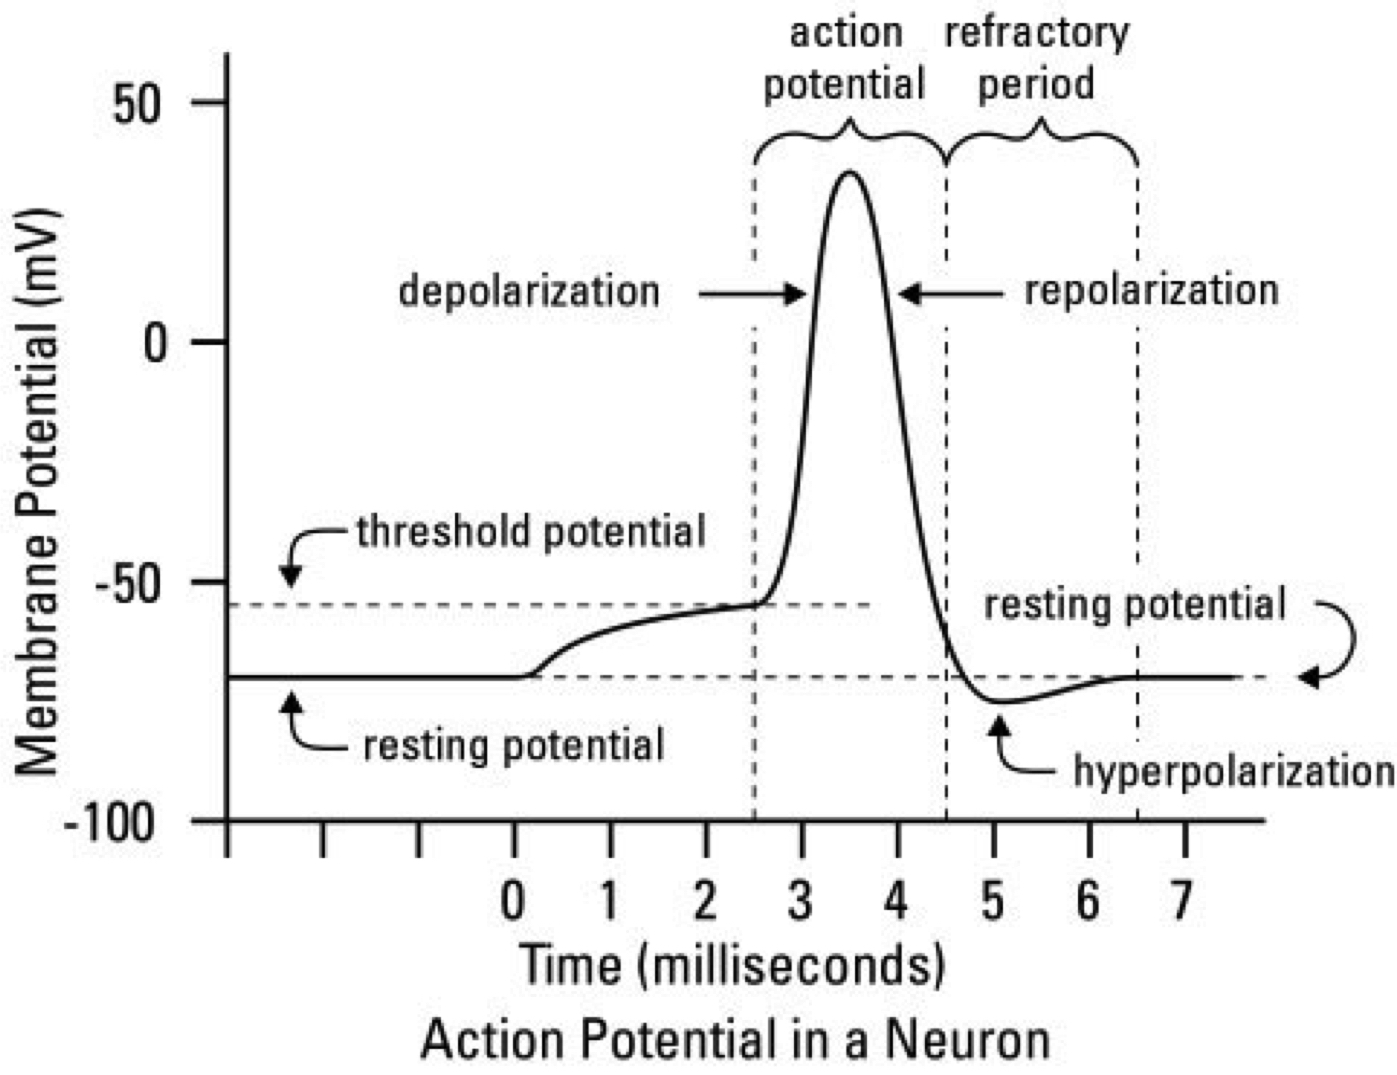
\includegraphics[width=.9\columnwidth]{AP_Actionpotential}
\end{minipage}%
\hspace{\boxmargin}%
\begin{minipage}{.65\columnwidth}
    \textbf{Four regimes during AP}:
    \begin{enumerate}
        \item[II] \textit{De}polarization:
        \ce{Na+} gate opens $\to$ \ce{Na+} in
        \item[III] \textit{Re}polarization:
        \ce{K+} gate opens $\to$ \ce{K+} out
        \item[IV] \textit{Hyper}polarization:\\
        Active \ce{Na+-K+-ion} pump (\ce{Na+}$\leftrightarrow$ \ce{K+})
    \end{enumerate}
\end{minipage}%
%%%%%%%%%%%%%%%%%%%%%%%%%%%%%%%%%%%%%%%%%%%%%%%%%%%%%%
\subsection{Decrement-free conduction}
%%%%%%%%%%%%%%%%%%%%%%%%%%%%%%%%%%%%%%%%%%%%%%%%%%%%%%
\subsubsection{Core -- Conductor Model}
%
\begin{minipage}{.3\columnwidth}
    \vspace{6mm}$V_m \big\downarrow$
    \begin{minipage}{.5\columnwidth}
        \vspace{-6mm}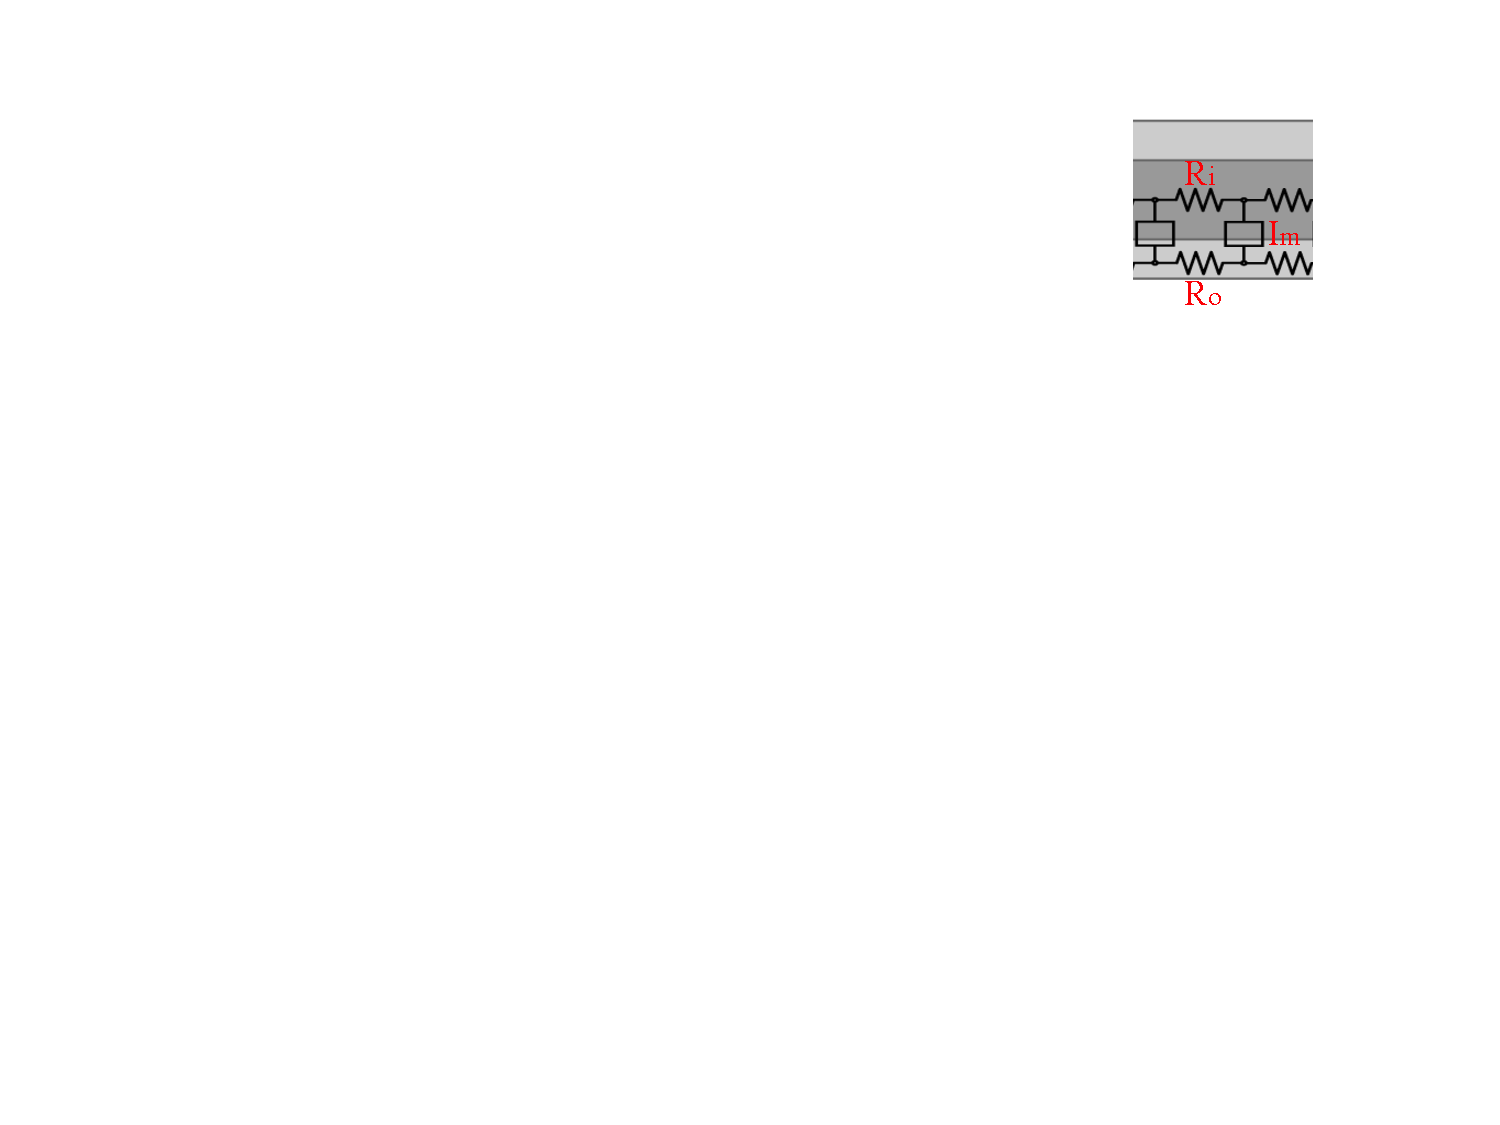
\includegraphics[width=\columnwidth]{AP_Core_Conductor_Model}
    \end{minipage}
\end{minipage}%
\hspace{1.5\boxmargin}%
\begin{minipage}{.6\columnwidth}
    $R_i = r_i \diff z$\quad $\leftarrow$ $\diff z$: per unit length\\
    $R_o = r_o \diff z$\\
    $I_m = k_m \diff z$\quad $\leftarrow$ may use HH-model
\end{minipage}%

\vspace{-3mm}
\formula{Core--Conductor eq.}{\pderiv[2]{V_m(z,t)}{z} = (r_o+r_i)K_m(z,t) - \overbrace{r_oK_e(z,t)}^{\overset{\textrm{if}}{=}\; 0 \;\to\; I_o = -I_i}}
\formula{\hfill wave eq.}{\phantom{\pderiv[2]{V_m(z,t)}{z}} = \frac{1}{v^2} \pderiv[2]{V_m(z,t)}{t} }
\enskip with $v = \frac{W}{\Delta t}$
\formbox{\hfill$\overset{K_e=0}{\implies}$}{v \simeq \frac{K_ma}{2\rho_i}}
\enskip for $r_i \gg r_o$
\enskip i.e. $v\propto\sqrt{a}$
%%%%%%%%%%%%%%%%%%%%%%%%%%%%%%%%%%%%%%%%%%%%%%%%%%%%%%
\subsubsection{Cable model \textnormal{-- Core--Conductor with HH-model inside}}
%
\formtex{Linearize \small(1st order)}{\small timescale for membrane voltage changes {$\tau_m {=} \frac{C_m}{G_m}$}}
\formtex{Cable equation}{Let $v_m = V_m + V_m\ap{rest}$}
~\qquad $v_m {+} \hspace{-1mm}\underbrace{\tau_m\pderiv{v_m}{t}\vspace{-1mm}}_{\vspace{-2mm} = 0 \text{ time indep.}}\hspace{-1mm} - \lambda_C^2 \pderiv[2]{v_m}{z} {=} r_o\lambda_C^2K_e$
\enskip \highlight{$\lambda_C {=} \frac{1}{\sqrt{g_m(r_o+r_i)}}$}
%%%%%%%%%%%%%%%%%%%%%%%%%%%%%%%%%%%%%%%%%%%%%%%%%%%%%%
\subsubsection{Saltatory Conduction Hypothesis}
%
$\to$ explain discrete manner in steps

\formula{velocity $\sim$ axon}{\textrm{total delay} \sim N (\#\textrm{nodes}) \sim (\textrm{axon length})/L}
\formula{diameter $D$}{\ce{->[$L\sim D$]} \textrm{velocity} \sim \frac{\textrm{total delay}}{\textrm{axon length}} \sim D}

\begin{minipage}{\columnwidth/3}
    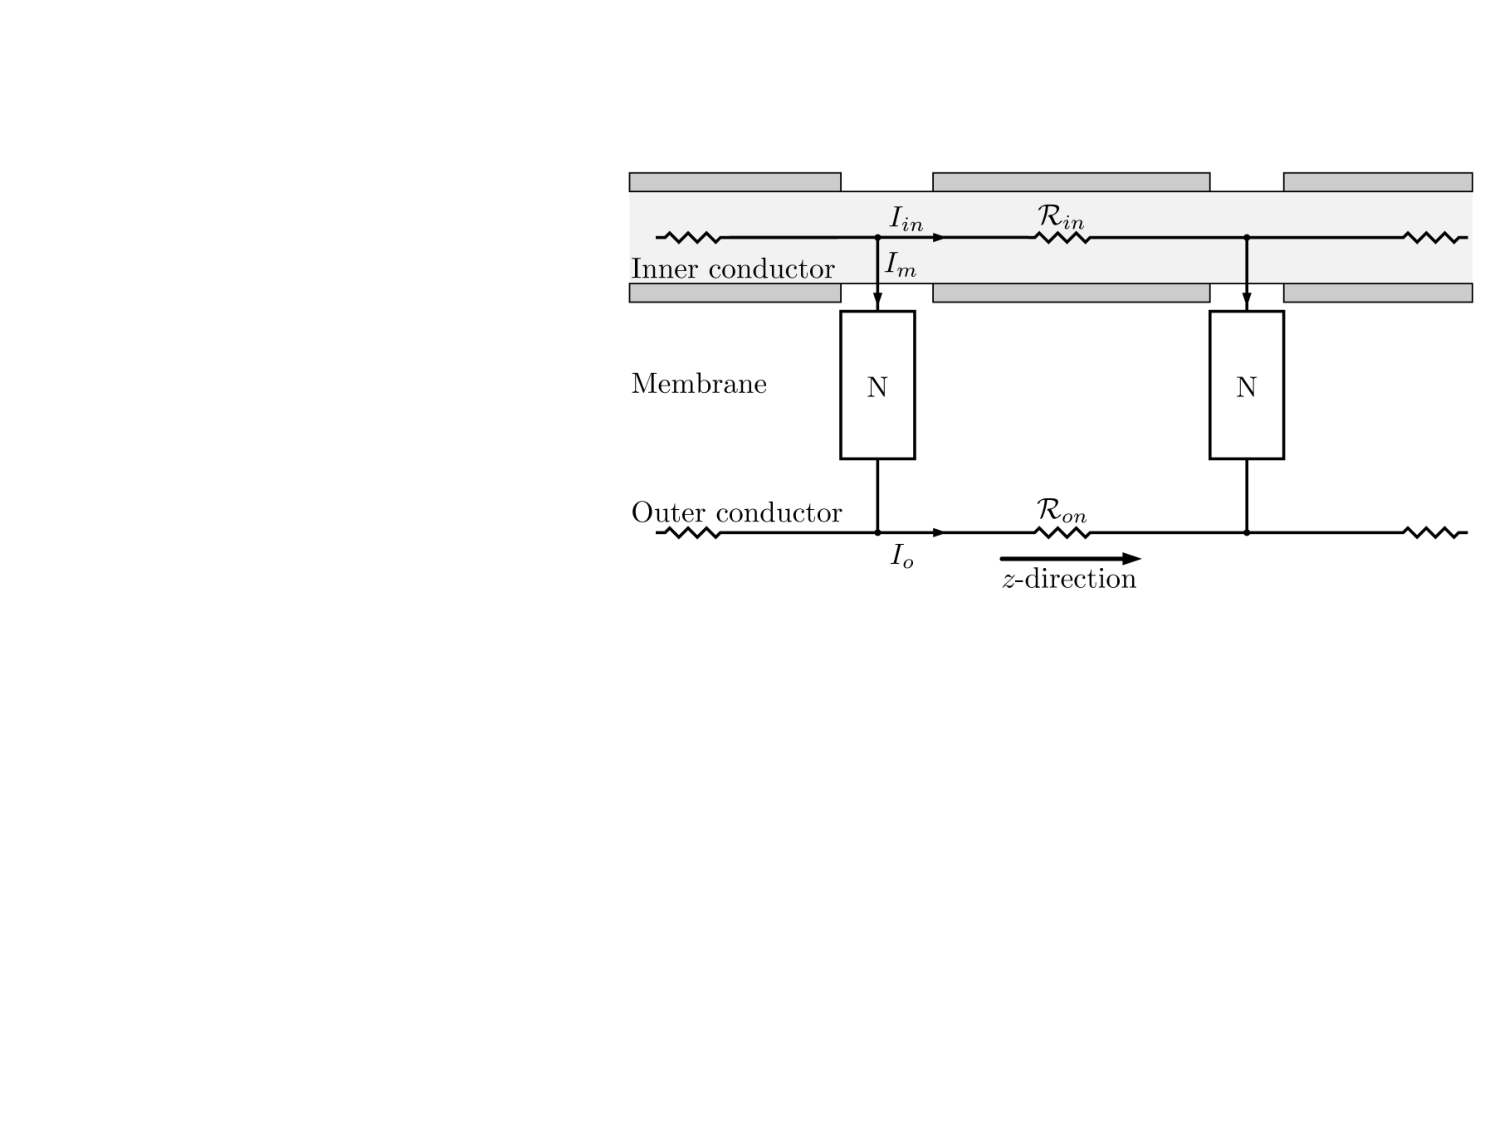
\includegraphics[width=.85\columnwidth]{AP_Saltatory}
\end{minipage}%
\begin{minipage}{\columnwidth/3}
    \centering
    \includegraphics[width=.8\columnwidth]{AP_Saltatory_2}
\end{minipage}%
\begin{minipage}{\columnwidth/3}
    \hfill
    \includegraphics[width=.75\columnwidth]{AP_Ranvier_Node}
\end{minipage}


	\end{multicols*}
\end{document}
